\secnumbersection{MARCO CONCEPTUAL}

%Se debe describir la base conceptual o fundamentos en los que se basa tu memoria, es decir, todos los conceptos técnicos, metodologías, herramientas, etc. que están involucradas en la solución propuesta. En el fondo esta parte permite precisar y delimitar el problema, estableciendo definiciones para unificar conceptos y lenguaje y fijar relaciones con otros trabajos o soluciones encontradas por otros al mismo problema evitando así plagios o repetir errores ya conocidos o abordados por otros.

%En esta parte es importante relacionar estos conceptos con la memoria y es fundamental utilizar referencias bibliográficas (o de la web) recientes, por ejemplo \cite{gettelfinger2004will}.

\subsection{Estado del Arte}

Las técnicas de \acrshort{ml} han sido utilizadas para solucionar todo tipo de problemas, un ejemplo que ha producido impacto es la aplicación en sistemas de recomendación, como el utilizado por la plataforma Netflix \cite{Koren2009}, para sugerir películas a los usuarios en base a la predicción de la calificación o \emph{rating} de las películas. Otra aplicación interesante es el estudio de obras de arte famosas, como \cite{Saleh2014}, en el que una red neuronal no supervisada determina la influencia entre los autores de diferentes pinturas.
%

En el campo de física de partículas, el uso de \acrshort{ml} se ha vuelto fundamental para el análisis de datos, debido a la necesidad de almacenar y analizar la cantidad creciente de datos acumulados \cite{Albertsson2018}. 
%
Existe una gran variedad de estudios en el área, que sentaron las bases en el uso de técnicas de \acrshort{ml}, un ejemplo es la búsqueda del bosón de Higgs con redes neuronales artificiales (\emph{artificial neural networks}, \acrshort{ann}) \cite{Chiappetta1994}, cuya labor consistió en clasificar los datos separándolos en dos grupos: \emph{background} y producción del bosón de Higgs. Otro ejemplo es el uso de \emph{boosted decision trees} (\acrshort{bdt}) y \acrshort{ann} para la identificación de partículas \cite{Roe2005}, resultando \acrshort{bdt} como el método más óptimo entre estos dos. También se tienen aplicaciones para la reconstrucción de trayectorias \cite{Peterson1989} y masas \cite{Lnnblad1992} de partículas utilizando \acrshort{ann}s entrenadas con datos de las señales captadas después de una colisión.
%
Particularmente, en el \acrshort{lhc}, el uso de \acrshort{ml} no está restringido sólo al estudio de las partículas, sino que es utilizado en el manejo de datos general, como en predicción del acceso a datos \cite{Kuznetsov2016} con el objetivo de optimizar el espacio de almacenamiento, además del monitoreo de la latencia en la transferencia de los datos \cite{Bonacorsi2015}, utilizando \acrshort{ml} para predecir congestiones e identificar fuentes problemáticas.
%
Con respecto al descubrimiento del bosón de Higgs, tanto \acrshort{atlas} \cite{Aad2012} \cite{Aad2012b} como \acrshort{cms} \cite{Chatrchyan2012} realizaron sus contribuciones utilizando algoritmos de \acrshort{ml} aplicados a conjuntos de datos reunidos en colisiones de partículas de máximo 7 TeV de energía.
%

Algunos ejemplos en los cuales las técnicas de \acrshort{ml} han sido aplicadas con éxito al análisis de los datos recogidos por el experimento \acrshort{atlas} son: la identificación de \emph{jets} hadrónicos producidos por quarks $b$ o leptones $\tau$ \cite{2016} \cite{ATLAS:2017mpa}, los cuales son fundamentales en el estudio de las propiedades físicas del bosón de Higgs. Dichas técnicas también han sido aplicadas en una variedad de búsquedas de nueva física, ya que permiten una mejor separación entre señal y background en procesos complicados, como es el caso de la producción del par de bosones de Higgs \cite{Aaboud2018}.
%

Durante el 2014 se realizó la competencia de \acrshort{ml} del bosón de Higgs \cite{Adam2015}, organizado por científicos de datos y físicos del experimento \acrshort{atlas}. Los participantes se enfrentaron para desarrollar un algoritmo en pos de mejorar la detección de eventos de señal del bosón de Higgs que decae en dos partículas $\tau$, utilizando una muestra de datos simulada de \acrshort{atlas} \cite{MLWP}. El ganador fue Gábor Melis \cite{Melis2015}, quien desarrolló un algoritmo de un conjunto de redes neuronales profundas (\emph{deep neural networks}, \acrshort{dnn}s) entrenadas con subconjuntos de datos aleatorios. El segundo ganador, Tim Salimans, desarrolló una solución descrita como la combinación de un gran número de \acrshort{bdt}s. La superioridad del método ganador que utiliza \acrshort{dnn} se justifica con su alta precisión y rapidez, sin embargo requiere de bastante capacidad computacional. Por otro lado, la solución de \acrshort{bdt}s presenta una solución más simple y requiere de menos recursos computacionales.
%

\emph{Deep learning} (\acrshort{dl} o {\em aprendizaje profundo}) es el enfoque actual de \acrshort{ml}, que está revolucionando el análisis de datos en diversas áreas de la ciencia, mejorando el estado del arte en reconocimiento de imágenes, investigación genómica, procesamiento del lenguaje natural y muchas otras áreas. Una aplicación bastante renombrada es \emph{DeepID3} \cite{Sun2015}, la cual consiste en una doble red neuronal profunda (\acrshort{dnn}) implementada para el reconocimiento facial. Otra aplicación es la de \emph{DeepBind} \cite{Park2015}, la cual propone una red neuronal profunda con convolución para predecir la afinidad de enlace entre una proteína y secuencias de \emph{ADN} o \emph{RNA}. Por último está \emph{DMN} (Red de Memoria Dinámica) \cite{Kumar2016}, que presenta una arquitectura de redes neuronales profundas entrenadas para recibir preguntas y devolver respuestas.
%
En particular, en el área de física de partículas, el enfoque \acrshort{dl} ha permitido obtener mayores niveles de desempeño en tareas de clasificación \cite{Guest2018}, como en la búsqueda de partículas exóticas\footnote{Partículas que se producen con muy baja frecuencia.} como el bosón de Higgs \cite{Baldi2014}, lo cual se traduce en la clasificación de eventos de física conocida y eventos de nueva física \cite{Bhimji2018}. Recientemente los físicos han enfocado su atención en implementar soluciones utilizando \acrshort{dl} para mejorar la sensibilidad del análisis, así como también para afrontar el incremento en la resolución de los datos generados por los detectores.
%

La literatura demuestra que los diversos problemas del \acrshort{lhc} han sido resueltos principalmente con técnicas de \acrshort{ml}, específicamente con redes neuronales artificiales (\acrshort{ann}) y boosted decision trees (\acrshort{bdt}) \cite{Radovic2018}, y más recientemente se ha innovado con el enfoque de \acrshort{dl}.

%*******************************%
%La mayoría de los ejemplos presentados anteriormente \red{requieren del conocimiento de un experto} 
% \sout{se relacionan con el uso de conocimiento de campo específico}%\footnote{Se refiere al estudio de un área específica o dominio de expertiz.} 
%\red{La extracción de características es una etapa fundamental ---y a la vez compleja--- en los algoritmos de machine learning, ya que las características definen a los datos y  deben lograr representar la complejidad del problema. }
%para la extracción de características de los datos y el diseño de las arquictecturas de las \acrshort{ann}s, con lo cual se pueden interpretar los datos usando un número determinado de características. 
%
%El problema es que en algunos casos, 
%\sout{se puede perder información al extraer} 
%\red{las} características \red{que definen los datos} que no capturan completamente la complejidad del problema. 

%
%En física de partículas se está realizando un gran esfuerzo para usar espacios de características de gran dimensión con los cuales entrenar algoritmos de \acrshort{ml} de última generación, como \acrshort{dnn}, \sout{cuya \textit{profundidad} de capas, lo cual será visto en las siguientes subsecciones,} es lo que permite extraer un gran número de características y, por ende, modelar transformaciones mucho más complicadas que las que son soportadas por las \acrshort{ann} \cite{Bengio2012}. 
%*******************************%

%\red{También elimino este párrafo, ya que ya se habló al comienzo de la sección de ANN, BDT y DL).}
%Debido a esto, la superioridad de cada método ha sido ampliamente debatida \cite{Derkach2018} \cite{Rogozhnikov2016}. Una sub-rama del \acrshort{ml} que ha tomado bastante fuerza en los últimos años, es Deep Learning (\acrshort{dl}), con métodos como Redes Neuronales Profundas \acrshort{dnn} \cite{Guest2018}. Sin duda, el excelente desempeño de las técnicas nombradas anteriormente, introduce el cuestionamiento: ¿Cuál es el mejor método para aplicar a este estudio? Para dar respuesta a esta pregunta es necesario internarse mayormente en el \acrshort{ml}. %

\subsection{Machine Learning}
%
Día a día, se generan gigantezcos volúmenes de datos; un claro ejemplo es Youtube, cuya plataforma procesa más de una hora de video por segundo. Para efectuar un análisis estadístico a tal cantidad de información, se requiere de métodos que automáticamente aprendan de los datos, es decir, programas que mejoren su desempeño con la experiencia \cite{Mitchell}, sin utilizar instrucciones programadas específicamente, y puedan realizar predicciones \cite{Murphy}, generando información nueva.
%
\acrshort{ml}, en esencia, corresponde a métodos de estadística aplicada, enfocados al uso de computación para estimar funciones matemáticas complejas, las cuales son posteriormente usadas para la extracción de información desde grandes cantidades de datos.

\subsubsection{Tipos de Aprendizaje}

Las técnicas de \acrshort{ml} son divididas en los siguientes tres principales tipos de aprendizaje:
%

\textbf{Aprendizaje supervisado:} 
%

El algoritmo debe ser capaz de inferir una función con la que sea capaz de predecir valores de salida para datos de entrada desconocidos \cite{Muller}. Esta función es estimada durante la fase de aprendizaje, efectuada durante el \textbf{entrenamiento} o \emph{training}, en el que el usuario provee al algoritmo un conjunto de datos con salida conocida, llamados \textbf{datos de entrenamiento}, que pueden representarse por la tupla $(x_i, y_i)$. Específicamente, $x_i$ es un dato de entrada y se expresa como un vector cuyas componentes son las características o atributos del dato. Por ejemplo, altura ($h$) y peso ($p$), caso en el que el vector $x_i$ se escribe como $<h_i,p_i>$, refiriéndose a la altura y peso del dato $i$. $y_i$ es la salida o etiqueta conocida de $x_i$. El presente trabajo se enfocará en el uso de algoritmos supervisados.
%

Los algoritmos supervisados se utilizan principalmente para resolver problemas de \textit{clasificación} y \textit{regresión} \cite{Murphy}. En el primero, el objetivo es predecir una categoría, por lo que la salida $y_i$ corresponde a un valor discreto. Mientras que en problemas de \textit{regresión} se busca predecir valores reales para la salida.
%

\textbf{Aprendizaje no supervisado:} 
%

El algoritmo recibe entradas no etiquetadas, es decir, el algoritmo debe aprender sin un \textit{educador} o supervisor. Son utilizados en tareas donde no se requiere de datos de ejemplo. Por ejemplo, en agrupación de datos (\emph{clustering}), identificación de patrones, algoritmos de visualización, reducción de dimensionalidad o detección de anomalías \cite{Bishop}.  
%

\textbf{Aprendizaje reforzado:} 
%

Es útil cuando se desea enseñar a un modelo a seguir cierto comportamiento a través de premios y castigos \cite{Bishop}. El sistema de aprendizaje, llamado \emph{agente}, puede "observar" su ambiente, seleccionar y efectuar acciones (de un conjunto predefinido), y obtener recomensas o penalizaciones. Así, el algoritmo debe aprender cuál es la mejor estrategia para obtener la mayor cantidad de recomensas posible \cite{Geron}. 

\subsubsection{Clasificación}
El objetivo del aprendizaje es generar una función $f$ que transforme las entradas $x_i$ en salidas $y_i \in C$, donde $C$ es el conjunto de clases. La función $f$ debe ser capaz de predecir la clase o etiqueta de un dato desconocido. Si el número de clases es dos, se habla de una \textbf{clasificación binaria} ---en la que usualmente se asume que las clases son $0$ y $1$--. Si hay más de dos clases, entonces se habla de \textbf{clasificación multiclase}. Si las clases no son mutuamente excluyentes, entonces es \textbf{clasificación multi-etiqueta} \cite{Murphy}.
%
Para el presente trabajo, al hablar de \textit{clasificación} se hace referencia a clasificación binaria.

\subsubsection{Representación de los Datos}
Para cualquier tipo de aprendizaje, es importante generar una \textit{representación de datos} que demuestre de forma clara cuáles son las \textbf{características} o propiedades que serán usadas para crear el modelo \cite{Muller}. Como se dijo anteriormente, los datos son representados por vectores y gráficamente como puntos en un espacio N-dimensional, donde N es la cantidad de características del conjunto de datos. Otra forma de representar los datos es usando una tabla \cite{Fernandes}, donde las columnas corresponden a las características y las filas a los datos, de esta forma las casillas de la tabla representan las mediciones de una característica para un dato determinado.
%

La Figura \ref{fig:scat} muestra una representación bi-dimensional de un conjunto arbitrario de datos de entrenamiento. La bi-dimensionalidad es simboliza que los datos se definen por dos características. Si un nuevo dato queda más cerca de la zona de los triángulos, el modelo lo etiquetará como clase \textit{triángulo} (clase 1), de lo contrario lo etiquetará como clase \textit{círculo} (clase 0). 
%
\begin{figure}[h]
  \centering
  \includegraphics[width=12cm]{figures/image11.png}
  \caption[Representación gráfica de un conjunto de datos de entrenamiento.]{Representación gráfica de un conjunto de datos de entrenamiento, con dos características (\emph{first feature} y \emph{second feature}), y dos categorías: \emph{class 0} y \emph{class 1}, simbolizadas por un círculo azul y un triángulo rojo respectivamente.
  \source{\cite[Capítulo 2]{Muller}}}
  \label{fig:scat}
\end{figure}

\subsubsection{\emph{Testing} y Validación}
El desempeño de los algoritmos de \acrshort{ml} se mide en la fase de \textbf{prueba} o \emph{testing}, en la que se utiliza como entrada un conjunto de datos etiquetados (\textbf{datos de testing}) y nuevos para el modelo. La habilidad de un algoritmo para desempeñarse eficientemente sobre los datos de \emph{testing}, se llama \textbf{generalización} \cite{Goodfellow}. Durante el entrenamiento, el modelo intenta minimizar su \textbf{error de entrenamiento}, correspondiente a la diferencia entre el valor de clasificación y la etiqueta real de cada dato. Sin embargo, para ver qué tan bien funciona el modelo, se debe evaluar el error utilizando los datos del conjunto de prueba, a este se le conoce como \textbf{error de generalización} o error de \emph{testing} \cite{Geron}.     
%
Si el error de entrenamiento es bajo y el error de generalización es alto, significa que el modelo está sobreajustando (\textbf{\emph{overfitting}}) los datos. El \emph{overfitting} ocurre básicamente debido a que el entrenamiento fue muy \textit{minucioso}, es decir que fueron consideradas variaciones muy pequeñas en la entrada, las cuales tienen más probabilidad de ser \textit{ruido} que \textit{señal real} \cite{Murphy}. Otro desafío al generar modelos de \acrshort{ml}, es minimizar el \textbf{\emph{underfitting}}, que, contrario al \emph{overfitting}, corresponde a cuando el entrenamiento fue demasiado \textit{simple}, es decir, el modelo no logra capturar eficientemente los patrones en los datos \cite{Raschka}, lo cual conduce a un bajo error de entrenamiento. La Figura \ref{fig:ovund} demuestra que el nivel de complejidad se relaciona directamente con el factor de \emph{overfitting} y \emph{underfitting} en un modelo.

\begin{figure}[h]
  \centering
  \includegraphics[width=11cm]{figures/image18.png}
  \caption[Representación de modelos con \emph{overfitting} y \emph{underfitting}.]{Representación de modelos con \emph{overfitting} y \emph{underfitting} en datos de entrenamiento. La sencillez del modelo con \emph{underfitting} produce grandes diferencias entre los valores predichos y los reales (\textit{alto sesgo}). Mientras que la complejidad del modelo con \emph{overfitting} genera valores predichos con mucha varianza.
  \source{\cite{Raschka}}}
  \label{fig:ovund}
\end{figure}

En resumen, el rendimiento de un algoritmo de \acrshort{ml} depende de dos factores:
\begin{itemize}
    \item Minimización del error de entrenamiento
    \item Minimización de la brecha entre el error de entrenamiento y el error de \emph{testing}.
\end{itemize}

Hay varias formas de prevenir el \emph{overfitting}, algunas de ellas son regularización, \emph{cross validation}, restricciones de norma máxima, \emph{dropout} (utilizada en \acrshort{ann}), entre otros \cite{Buduma}.

\subsubsection{Clasificadores}

\blue{To do.}

\subsection{Boosted Decision Trees}

\subsubsection{Árboles de Clasificación}

Los árboles de decisión son algoritmos de \acrshort{ml} utilizados para tareas de clasificación y regresión, capaces de procesar conjuntos de datos complejos \cite{Geron}.
%
Como su nombre lo indica, emplean un modelo de decisiones en forma de árbol, y una característica principal es que divide un proceso complejo de toma de decisiones en un conjunto de decisiones más simples \cite{Safavian}.
%
La Figura \ref{fig:tree1} muestra un ejemplo de un árbol de decisión. 
%
Cada uno de los \textit{rectángulos} corresponde a un \textbf{nodo} y representa la verificación de cierta característica de los datos, por ejemplo, en el caso de que un dato se refiere a un animal, una posible verificación sería \textit{"¿Puede volar?"}. Estas verificaciones son llamadas \textit{nodos test} \cite{Muller}. 
%
Las ramas que conectan los nodos corresponden a los posibles valores de la verificación, por ejemplo "\textit{Sí/No}" \cite{Mitchell}. Generalmente las verificaciones utilizan operaciones de tipo $=$ y $\neq$ para el caso en el que las entradas categóricas sean discretas, y $<$, $\ge$, $>$ o $\le$ para entradas de valor continuo. Los valores de la verificación son representados por números, por ejemplo $1$ (``Sí'') y $0$ (``No''), para divisiones binarias, aunque también puede haber separaciones de tres niveles o más.
%

El recorrido de un árbol de decisión comienza por su raíz (o \emph{root}), desde donde el conjunto de datos será dividido en dos (o más) sub-conjuntos, en base a una verificación (o pregunta) con respecto a una característica.
%
Este proceso se vuelve a repetir con los sub-conjuntos como entradas de los nodos que siguen hasta que se hayan cubierto todas características de los datos y no puedan realizarse más verificaciones. 
%
Los sub-conjuntos resultantes son llamados \textbf{hojas}. 
%

En la Figura \ref{fig:tree1} los datos (probablemente correspondientes a animales) tienen las siguientes características: "[Sí/No tiene plumas, Sí/No puede volar, Sí/No tiene aletas]", junto con la etiqueta (especie) correspondiente: ``Halcón'', ``Pingüino'', ``Delfín'' y ``Oso''.

\begin{figure}[h]
  \centering
  \includegraphics[width=12cm]{figures/image12.jpg}
  \caption[Esquema de árbol de decisión para clasificar animales.]{Esquema de árbol de decisión para clasificar a un animal entre las especies; halcón, pingüino, delfín u oso, aplicando las verificaciones; "¿tiene alas?", seguido de "¿puede volar?" ó "¿tiene aletas?".
  \source{Elaboración propia, basada en ejemplo de \cite[Capítulo 2]{Muller}.}}
  \label{fig:tree1}
\end{figure}

Para hacer una predicción con un dato nuevo, se debe atravesar el árbol desde la raíz hasta llegar a una de las hojas, la cual corresponde a una etiqueta o valor de predicción. Una predicción para el árbol de la Figura \ref{fig:tree1}, se puede ejemplificar con la Figura \ref{fig:tree2}.

\begin{figure}[h]
  \centering
  \includegraphics[width=13cm]{figures/image13.jpg}
  \caption[Esquema de árbol de decisión para clasificar un nuevo dato (de tipo \textit{animal}).]{Esquema de árbol de decisión para clasificar un nuevo dato cuyas características tienen los valores: ["Sí, tiene plumas", "No puede volar", "Sí, tiene aletas"]. El camino que sigue el dato dentro del árbol está marcado con las flechas rojas, terminando en la clase "Pingüino", que sería la etiqueta final del dato ingresado.
  \source{Elaboración propia, basada en ejemplo de \cite[Capítulo 2]{Muller}}.}
  \label{fig:tree2}
\end{figure}

\subsubsection{Entrenamiento}
Durante el entrenamiento, el algoritmo será capaz de encontrar la secuencia adecuada de verificaciones o preguntas que proporcionen la respuesta correcta en la menor cantidad de pasos \cite{Muller}. Si un sub-conjunto final del árbol, es decir una hoja, posee datos que tengan la misma etiqueta, entonces se dice que esa hoja es \textit{pura}, y el que todas las hojas sean \textit{puras}, indica que el árbol tiene una presición del 100$\%$.

Con el objetivo de encontrar esta secuencia ideal de verificaciones para dividir los datos, se usan heurísticas que eligen las mejores características y valores de estas, como base para sugerir verificaciones o particiones. Sumado a esto, la calidad de una verificación propuesta, se mide respondiendo a las cuestionantes: \textit{¿El árbol tiene una profundidad adecuada?} \textit{¿La distribución entre los subconjuntos generados en el nodo, es lo suficientemente homogénea?} \textit{¿El tamaño de los subconjuntos es lo suficientemente grande?} \cite[Capítulo 16]{Murphy}. Estas preguntas pueden ser respondidas en base al valor de diferentes medidas de error.
%
\subsubsection{Costo de Clasificación}
Para evaluar la calidad de las particiones propuestas se pueden medir los siguientes errores \cite{Murphy}:

\textbf{Taza de Clasificación Errónea:} Es el promedio de datos mal clasificados en un nodo. Siendo $D$ el conjunto de datos del nodo, $y_i$ es la clasificación real del dato $i$, $\hat{y}$ es la predicción de la clase del dato $i$, y $\mathbb{I}$ es la función \textit{indicatriz} que retorna $1$ si se cumple que la clasificación y la predicción de la clase del dato $i$ coinciden.
\begin{align}
 \frac{1}{|D|} \sum_{i \in D} \mathbb{I}(y_i \neq \hat{y})
\end{align} 

\textbf{Entropía:} Permite calcular la homogeneidad de las predicciones en un nodo. Si hay homogeneidad total, el valor de la entropía es $0$, de lo contrario es $1$. Siendo $\hat{\pi}$ es una variable aleatoria cuyos valores son las clases, $C$ es el conjunto de clases, $\hat{\pi}_c$ es la probabilidad de que una predicción coincida con la clase $c$, dada la verificación del nodo.
\begin{align}
 \mathbb{H}(\hat{\pi}) = -\sum_{c \in C} \hat{\pi}_c \log(\hat{\pi}_c)
\end{align} 

\textbf{Índice Gini:} Es la tasa de error esperado, donde $(1-\hat{\pi}_c)$ es la probabilidad de que una predicción para la clase $c$ resulte errónea.
\begin{align}
 \sum_{c \in C} \hat{\pi}_c (1-\hat{\pi}_c)
\end{align} 

La secuencia y posición de las verificaciones o \emph{nodos test} son esenciales para determinar el desempeño del árbol de decisión, es por ello que se pueden obtener mejores niveles de precisión si se utilizan múltiples árboles de decisión \cite{Quinlan1996}, con diferentes estructuras que otorguen mayor flexibilidad a la clasificación. 
%
Por otro lado, pese a que los árboles de decisión entregan buenos resultados, también son inestables, ya que un pequeño cambio en los datos de entrenamiento puede desencadenar muchos cambios en el árbol \cite{Roe2005}. 
%
Estas son dos de las situaciones que los algoritmos de \textit{boosting} intentan mejorar. 
%
\subsubsection{\emph{Boosting}}

En los algoritmos de \emph{boosting}, se seleccionan, de forma aleatoria y con repetición, subconjuntos de datos a partir del conjunto de entrenamiento. Los subconjuntos son ordenados de forma secuencial y cada uno se ajusta a un árbol de decisión diferente \cite{James}. Los datos de entrenamiento que fueron mal clasificados durante la fase de \textit{testing} o prueba de un árbol, serán considerados en el siguiente con pesos más grandes. Estos árboles son conocidos como árboles \emph{boosted} o \emph{boosted trees}. 
%

Los algoritmos de \emph{boosting} tienen 3 parámetros de ajuste \cite{James}:
\begin{itemize}
    \item \textbf{Número de árboles (B):} Si B es muy grande, se puede producir \emph{overfitting}.
    \item \textbf{Parámetro de encogimiento (\lambda):} Controla la tasa de aprendizaje del algoritmo. Normalmente se usan valores de $0.01$ o $0.001$. Un valor pequeño de \lambda puede requerir un valor grande de B.
    \item \textbf{Número de divisiones en cada árbol ($d$):} Controla la complejidad del grupo de árboles. A menudo se usa un valor de $d=1$ implica que el árbol tiene sólo una ramificación, ya que un árbol con $d$ divisiones tiene $d$ variables.
\end{itemize}
%
Según lo anterior, los \emph{Boosted Decision Trees} (\acrshort{bdt}) son conjuntos de árboles de decisión que usan técnicas de \emph{boosting}. 
%
Un \acrshort{bdt} implementado para clasificación binaria utiliza un sistema de puntaje para predecir la etiqueta de datos nuevos. 
%
Este consiste en que cuando un dato que es procesado por un árbol de tipo \emph{boosted}, cae en una \textit{hoja} de la \textit{primera clase}, obtiene un puntaje de $1$, pero al caer en hojas de la \textit{segunda clase}, obtiene un puntaje de $-1$. Al pasar por todos los árboles \emph{boosted}, el puntaje definitivo será la suma de todos los puntajes obtenidos. Si este es un valor muy grande, el dato será etiquetado como \textit{primera clase}, y si el valor es muy pequeño, será etiquetado como \textit{segunda clase}. Esto se determina con la ayuda de un valor de \textit{umbral} o \emph{threshold} de referencia, previamente definido. 
%
%
\subsection{Redes Neuronales Artificiales y Aprendizaje Profundo}
%
Las redes neuronales artificiales (o \acrshort{ann}s, del inglés artificial neural networks) son modelos computacionales inspirados en las redes de neuronas biológicas del sistema nervioso central \cite{Graupe}. Están compuestas de un cojunto de unidades o nodos denominados \textit{neurona artificial}, la cual modela de forma muy simple la neurona del cerebro biológico. 
%
%\sout{Además, permiten usar operaciones computacionales simples, (sumas, multiplicaciones y elementos lógicos fundamentales) para resolver problemas complejos de tipo estocástico o no lineales.}
%
%
%
%An ANN is based on a collection of connected units or nodes called artificial neurons, which loosely model the neurons in a biological brain. Each connection, like the synapses in a biological brain, can transmit a signal from one artificial neuron to another. An artificial neuron that receives a signal can process it and then signal additional artificial neurons connected to it.
%
%\sout{La unidad fundamental de} 
%\red{La neurona del} cerebro 
%\sout{es la \textit{neurona}, la cual} 
%tiene en promedio seis mil conexiones con otras neuronas y es el medio a través del cual los seres humanos aprenden de su entorno. 
%
%Esta unidad es utilizada como base para construir modelos de redes neuronales \cite{Buduma} que pueden ser representados en computador.
%
%
\subsubsection{La Neurona}

Como se muestra en la Figura \ref{fig:neur}, la neurona artificial toma el conjunto de \textbf{entradas} $x_0$, $x_1$,..., $x_n$, cada una multiplicada por un \textbf{peso} específico del conjunto $w_0$, $w_1$,..., $w_n$. Los conjuntos de entradas y pesos se expresan como los vectores \textbf{$x$} y \textbf{$w$} respectivamente. El término $x_i w_i$ se conoce como \textit{entrada ponderada}, las cuales son sumadas para formar el \textbf{logit} (o suma ponderada) $z = \sum_{i=0}^n {x_i w_i} = $ \textbf{$x w$}. En muchos casos también se considera un \textit{sesgo} ($b$), donde la fórmula del \emph{logit} sería $z = b + \sum_{i=0}^n {x_i w_i}$. Para el caso específico de la neurona en la Figura \ref{fig:neur}, el logit es $z = x_1 w_1 + x_2 w_2 + x_3 w_3$. Luego, la neurona realiza un cálculo utilizando la función $f$, llamada \textbf{función de activación}, sobre el \emph{logit} para producir la \textbf{salida} $y = f(z)$ \cite{Bishop}. Este proceso se repite pasando la salida $y$ como entrada a otra(s) neurona(s).

Las neuronas artificiales se pueden clasificar según su función de activación \cite{Buduma}:
\begin{itemize}
    \item[$\bullet$] \textit{Neuronas Lineales}: Tienen funciones de activación lineales, en la forma $f(z) = az + b$.  
    \item[$\bullet$] \textit{Neuronas Sigmoide}: Usan la función de activación $f(z)=\displaystyle\frac{1}{1+e^{-z}}$. Esto significa que cuando el logit es muy pequeño, la salida de una neurona es cercana a cero. Y cuando el logit es muy grande, la salida será cercana a uno. Su gráfico se puede observar en la Figura \ref{fig:sigm}.
    \item[$\bullet$] \textit{Neuronas Tangente Hiperbólico}: Tienen una forma parecida a las neurones sigmoides. Su función de activación es $f(z)=tanh(z)=\displaystyle\frac{e^{z}-e^{-z}}{e^{z}+e^{-z}}$. La salida se mueve en el rango de cero a uno, y la función $f$ va desde $-1$ a $1$, como se observa en la Figura \ref{fig:tanh}.
    \item[$\bullet$] \textit{Neurona \acrshort{relu}}: Usa la función $f(z)=max(0,z)$, lo que quiere decir que deja pasar a todos los valores positivos sin cambiarlos, pero transforma los valores negativos a cero. Su gráfico se puede observar en la Figura \ref{fig:relu}.  
\end{itemize}

\begin{figure}[h]
\centering
\begin{subfigure}[b]{.45\linewidth}
\includegraphics[width=\linewidth]{figures/image15.png}
\caption{Neurona Sigmoide}\label{fig:sigm}
\end{subfigure}
\begin{subfigure}[b]{.45\linewidth}
\includegraphics[width=\linewidth]{figures/image16.png}
\caption{Neurona Tanh}\label{fig:tanh}
\end{subfigure}
\begin{subfigure}[b]{.45\linewidth}
\includegraphics[width=\linewidth]{figures/image17.png}
\caption{Neurona ReLU}\label{fig:relu}
\end{subfigure}
\caption[Neuronas de función no lineal.]{Neuronas de función no lineal.
\source{\cite{Buduma}}}
\label{fig:main}
\end{figure}

\begin{figure}[h]
\centering
\tikzset{every picture/.style={line width=0.75pt}} %set default line width to 0.75pt        

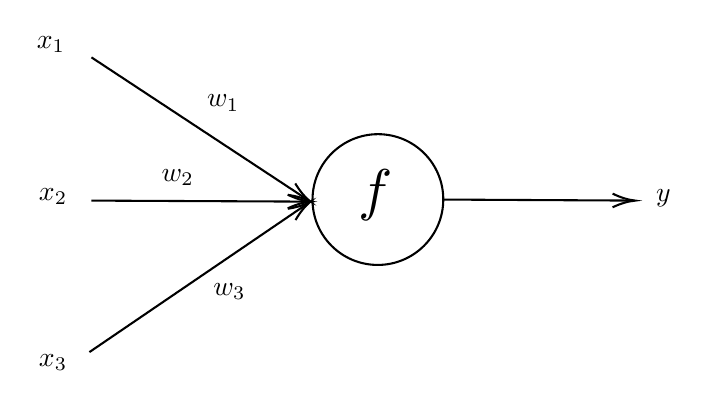
\begin{tikzpicture}[x=0.75pt,y=0.75pt,yscale=-1,xscale=1]
%uncomment if require: \path (0,194); %set diagram left start at 0, and has height of 194

%Shape: Circle [id:dp058244464473876545] 
\draw   (144.99,88.5) .. controls (145.03,71.1) and (159.17,57) .. (176.57,57) .. controls (193.97,57) and (208.03,71.1) .. (207.99,88.5) .. controls (207.94,105.9) and (193.8,120) .. (176.41,120) .. controls (159.01,120) and (144.94,105.9) .. (144.99,88.5) -- cycle ;
%Straight Lines [id:da46924522998984264] 
\draw    (38.5,89) -- (141.99,89.49) ;
\draw [shift={(143.99,89.5)}, rotate = 180.27] [color={rgb, 255:red, 0; green, 0; blue, 0 }  ][line width=0.75]    (10.93,-3.29) .. controls (6.95,-1.4) and (3.31,-0.3) .. (0,0) .. controls (3.31,0.3) and (6.95,1.4) .. (10.93,3.29)   ;

%Straight Lines [id:da764532034401557] 
\draw    (38.5,20) -- (142.32,88.4) ;
\draw [shift={(143.99,89.5)}, rotate = 213.38] [color={rgb, 255:red, 0; green, 0; blue, 0 }  ][line width=0.75]    (10.93,-3.29) .. controls (6.95,-1.4) and (3.31,-0.3) .. (0,0) .. controls (3.31,0.3) and (6.95,1.4) .. (10.93,3.29)   ;

%Straight Lines [id:da33196562179949296] 
\draw    (207.99,88.5) -- (298.5,88.99) ;
\draw [shift={(300.5,89)}, rotate = 180.31] [color={rgb, 255:red, 0; green, 0; blue, 0 }  ][line width=0.75]    (10.93,-3.29) .. controls (6.95,-1.4) and (3.31,-0.3) .. (0,0) .. controls (3.31,0.3) and (6.95,1.4) .. (10.93,3.29)   ;

%Straight Lines [id:da4624390017909269] 
\draw    (37.5,162) -- (142.33,90.63) ;
\draw [shift={(143.99,89.5)}, rotate = 505.75] [color={rgb, 255:red, 0; green, 0; blue, 0 }  ][line width=0.75]    (10.93,-3.29) .. controls (6.95,-1.4) and (3.31,-0.3) .. (0,0) .. controls (3.31,0.3) and (6.95,1.4) .. (10.93,3.29)   ;


% Text Node
\draw (102,42) node  [align=left] {$w_1$};
% Text Node
\draw (175.49,86.5) node [scale=2.074]  {${\displaystyle f}$};
% Text Node
\draw (80,78) node  [align=left] {$w_2$};
% Text Node
\draw (105,133) node  [align=left] {$w_3$};
% Text Node
\draw (19,14) node  [align=left] {$x_1$};
% Text Node
\draw (20,87) node  [align=left] {$x_2$};
% Text Node
\draw (20,167) node  [align=left] {$x_3$};
% Text Node
\draw (314,88) node  [align=left] {$y$};

\end{tikzpicture}
\caption[Esquema de una neurona en una red neuronal artificial.]{Esquema de una neurona en una red neuronal artificial. En ella, $x_i$ son las entradas de la neurona, $w_i$ son los \textit{pesos} para cada entrada, $f$ es la función que aplica la neurona sobre las \textit{entradas ponderadas} e $y$ es la salida de la neurona.
\source{Elaboración propia.}} 
\label{fig:neur}
\end{figure}

\subsubsection{Estructura de una Red}

En el cerebro, las neuronas están organizadas en capas, y la información fluye de una capa a otra, hasta que las entradas sensoriales son transformadas en entendimiento conceptual. 
%
En este contexto, las redes neuronales artificiales son construidas conectando neuronas y formando capas de estas. 
%
Se tienen tres tipos de capas \cite{Buduma}:

\textbf{Capa de entrada:} Corresponde al grupo de neuronas que introduce los datos a la red. Los nodos que conforman esta capa son llamados \textit{unidades de entrada}. Estas no procesan información, sino que sólo la traspasan a otras unidades.

\textbf{Capa oculta:} Sus nodos son llamados \textit{unidades ocultas}. Se ubican entre la capa de entrada y la capa de salida, y no son directamente observables.

\textbf{Capa de salida:} Sus nodos son llamados \textit{unidades de salida}. Codifican posibles valores para la instancia. Por ejemplo, cada unidad de salida puede representar una de las categorías.
% Tipos de funciones (softmax, etc).

Desde el punto de vista del esquema general de conexiones entre las  unidades, una red puede ser \emph{feedforward} o \textit{recurrente}, y la conexión entre dos neuronas o unidades, puede ser \textit{simétrica} o \textit{asimétrica} \cite{Fu}.
\begin{itemize}
    \item \textit{Red Feedforward:} Todas las conexiones tienen una misma dirección, desde la capa de entrada hacia la capa de salida.
    \item \textit{Red Recurrente:} Hay conexiones que forman ciclos.
    \item \textit{Conexiones Simétricas:} La conexión entre dos neuronas es bidireccional y el peso asociado a esa conexión es el mismo para ambas unidades.
    \item \textit{Conexiones Asimétricas:} La conexión entre dos neuronas es unidireccional.
\end{itemize}

\subsubsection{Representación}

Una neurona individual realiza operaciones vectoriales para procesar sus pesos y entradas entre dos nodos. En una red neuronal, estas operaciones son representadas usando matrices y vectores. Considerando $N_k$ como el número de neuronas en la capa $k$ y $P$ como el número total de capas, la simbología y su representación se describen a continuación:

\textbf{Pesos:}
\begin{itemize}
    \item $W^{(k)}$: Matriz de pesos para las conexiones entre la capa $(k-1)$ y $k$ de la red.
    \item $w_{j}^{(k)}$: Vectores columna de $W^{(k)}$. Representan los pesos que llegan a la neurona $j$ de la capa $k$. 
    \item $w_{i,j}^{(k)}$: Componentes escalares del vector $w_{j}^{(k)T}$. Representan los pesos de la conexión entre la neurona $i$ de la capa $(k-1)$ y la neurona $j$ de la capa $k$.
\end{itemize} 
%
Es importante acotar que la capa de entrada no tiene pesos.
%
\begin{align*}
    W^{(k)} = \begin{bmatrix} 
                w_{1}^{(k)T} \\ 
                w_{2}^{(k)T} \\ 
                \vdots \\ 
                w_{N_k}^{(k)T} 
              \end{bmatrix} 
            = \begin{bmatrix} 
                w_{1,1}^{(k)} & w_{2,1}^{(k)} & \dots & w_{N_k,1}^{(k)} \\
                w_{1,2}^{(k)} & w_{2,2}^{(k)} & \dots & w_{N_k,2}^{(k)} \\
                \vdots & & \ddots & \vdots \\
                w_{1,N_k}^{(k)} & w_{2,N_k}^{(k)} & \dots & w_{N_k,N_k}^{(k)}
              \end{bmatrix}
\end{align*}

\textbf{Entradas:}
\begin{itemize}
    \item $A^{(k)}$: Vector columna equivalente las entradas de la capa $k$.
    \item $a_{i}^{(k)}$: Componentes escalares de $A^{(k)}$. Corresponde al dato de entrada $i$ de la capa $k$.
\end{itemize}
%
Se debe considerar que los datos de entrada de la capa de entrada, son los datos originales. Por otro lado, los datos de entrada $a_{i}^{(k)}$ de una capa oculta o capa de salida ($k$), son los datos de salida de la capa anterior, es decir $a_{i}^{(k)} = f(z_{i}^{(k)})$.
%
\begin{align*}
    A^{(k)} = \begin{bmatrix} 
                a_{1}^{(k)} \\ 
                a_{2}^{(k)} \\ 
                \vdots \\ 
                a_{N_k}^{(k)} 
              \end{bmatrix}
            = f(Z^{(k)})
            = \begin{bmatrix} 
                f(z_{1}^{(k)}) \\ 
                f(z_{2}^{(k)}) \\ 
                \vdots \\ 
                f(z_{N_k}^{(k)}) 
              \end{bmatrix}
            = \begin{bmatrix} 
                f(w_{1}^{(k)T} A^{k-1} + b_1^{(k)}) \\ 
                f(w_{2}^{(k)T} A^{k-1} + b_2^{(k)}) \\ 
                \vdots \\ 
                f(w_{N_k}^{(k)T} A^{k-1} + b_{N_k}^{(k)}) 
              \end{bmatrix}
\end{align*}
%

\textbf{Suma ponderada:}
\begin{itemize}
    \item $Z^{(k)}$: Vector de las sumas ponderadas (\emph{logits}) en la capa $k$.
    \item $z_i^{(k)}$: Componentes escalares de $Z^{(k)}$. Representa el \emph{logit} de la neurona $i$ de la capa $k$ y equivale a la operación vectorial $w_j^{(k)T} A^{k-1} + b_i^{(k)}$
\end{itemize}
%
\begin{align*}
    Z^{(k)} = \begin{bmatrix} 
                z_1^{(k)} \\ 
                z_2^{(k)} \\ 
                \vdots \\ 
                z_{N_k}^{(k)} 
              \end{bmatrix}
            = \begin{bmatrix} 
                w_{1}^{(k)T} A^{k-1} + b_1^{(k)} \\ 
                w_{2}^{(k)T} A^{k-1} + b_2^{(k)} \\ 
                \vdots \\ 
                w_{N_k}^{(k)T} A^{k-1} + b_{N_k}^{(k)} 
              \end{bmatrix}
\end{align*}
%

\textbf{Sesgo:}
\begin{itemize}
    \item $b^{(k)}$: Vector de los sesgos en la capa $k$.
    \item $b_i^{(k)}$: Componentes escalares de $b^{(k)}$. Corresponde al sesgo de la neurona $i$ en la capa $k$.
\end{itemize}
%
\begin{align*}
    b^{(k)} = \begin{bmatrix} 
                b_1^{(k)} \\ 
                b_2^{(k)} \\ 
                \vdots \\ 
                b_{N_k}^{(k)} 
              \end{bmatrix}
\end{align*}
%

En la red neuronal de la Figura \ref{fig:ann1}, las matrices de pesos y los vectores de entradas se definen de la siguiente forma.
%
\begin{figure}[h]
\centering
\tikzset{every picture/.style={line width=0.75pt}} %set default line width to 0.75pt        
\resizebox{11cm}{6cm}{

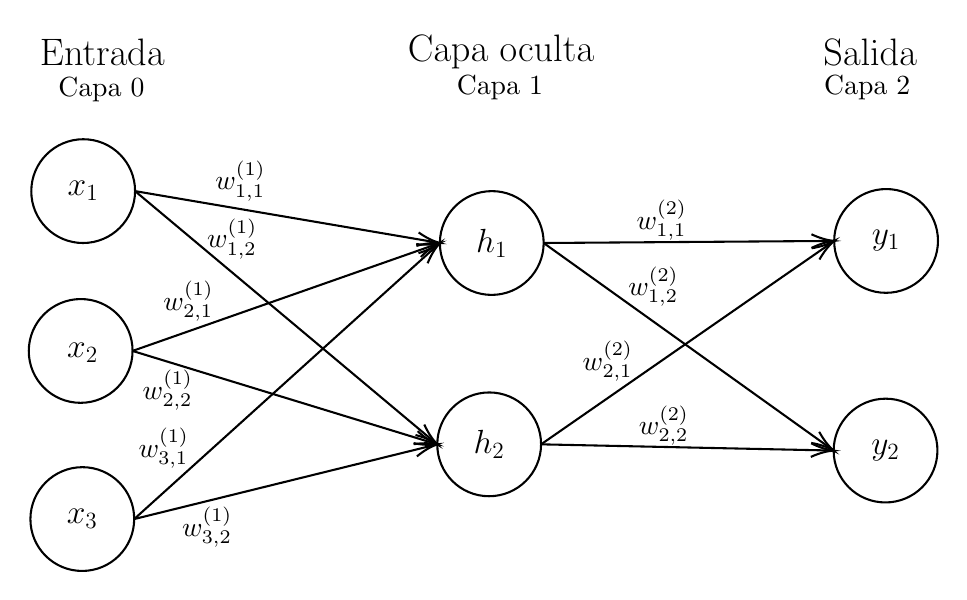
\begin{tikzpicture}[x=0.75pt,y=0.75pt,yscale=-1,xscale=1]
%uncomment if require: \path (0,398); %set diagram left start at 0, and has height of 398

%Shape: Circle [id:dp014797891854668621] 
\draw   (44.21,86) .. controls (44.24,72.19) and (55.46,61) .. (69.27,61) .. controls (83.08,61) and (94.24,72.19) .. (94.21,86) .. controls (94.17,99.81) and (82.95,111) .. (69.14,111) .. controls (55.33,111) and (44.17,99.81) .. (44.21,86) -- cycle ;
%Shape: Circle [id:dp058244464473876545] 
\draw   (43,163) .. controls (43.04,149.19) and (54.26,138) .. (68.07,138) .. controls (81.88,138) and (93.04,149.19) .. (93,163) .. controls (92.97,176.81) and (81.75,188) .. (67.94,188) .. controls (54.13,188) and (42.97,176.81) .. (43,163) -- cycle ;
%Shape: Circle [id:dp31737473014049844] 
\draw   (43.79,244) .. controls (43.83,230.19) and (55.05,219) .. (68.86,219) .. controls (82.67,219) and (93.83,230.19) .. (93.79,244) .. controls (93.76,257.81) and (82.53,269) .. (68.73,269) .. controls (54.92,269) and (43.76,257.81) .. (43.79,244) -- cycle ;
%Shape: Circle [id:dp014201185840476138] 
\draw   (431.05,110) .. controls (431.09,96.19) and (442.31,85) .. (456.12,85) .. controls (469.93,85) and (481.09,96.19) .. (481.05,110) .. controls (481.02,123.81) and (469.8,135) .. (455.99,135) .. controls (442.18,135) and (431.02,123.81) .. (431.05,110) -- cycle ;
%Shape: Circle [id:dp7248329472734] 
\draw   (430.79,211) .. controls (430.83,197.19) and (442.05,186) .. (455.86,186) .. controls (469.66,186) and (480.83,197.19) .. (480.79,211) .. controls (480.75,224.81) and (469.53,236) .. (455.72,236) .. controls (441.92,236) and (430.75,224.81) .. (430.79,211) -- cycle ;
%Straight Lines [id:da23388739067292408] 
\draw    (93,163) -- (239.18,111.66) ;
\draw [shift={(241.07,111)}, rotate = 520.65] [color={rgb, 255:red, 0; green, 0; blue, 0 }  ][line width=0.75]    (10.93,-3.29) .. controls (6.95,-1.4) and (3.31,-0.3) .. (0,0) .. controls (3.31,0.3) and (6.95,1.4) .. (10.93,3.29)   ;

%Straight Lines [id:da46924522998984264] 
\draw    (93.79,244) -- (239.59,112.34) ;
\draw [shift={(241.07,111)}, rotate = 497.92] [color={rgb, 255:red, 0; green, 0; blue, 0 }  ][line width=0.75]    (10.93,-3.29) .. controls (6.95,-1.4) and (3.31,-0.3) .. (0,0) .. controls (3.31,0.3) and (6.95,1.4) .. (10.93,3.29)   ;

%Straight Lines [id:da5852104107316262] 
\draw    (94.21,86) -- (239.1,110.66) ;
\draw [shift={(241.07,111)}, rotate = 189.66] [color={rgb, 255:red, 0; green, 0; blue, 0 }  ][line width=0.75]    (10.93,-3.29) .. controls (6.95,-1.4) and (3.31,-0.3) .. (0,0) .. controls (3.31,0.3) and (6.95,1.4) .. (10.93,3.29)   ;

%Shape: Circle [id:dp7916193742410371] 
\draw   (241.07,111) .. controls (241.11,97.19) and (252.33,86) .. (266.14,86) .. controls (279.94,86) and (291.11,97.19) .. (291.07,111) .. controls (291.03,124.81) and (279.81,136) .. (266,136) .. controls (252.2,136) and (241.03,124.81) .. (241.07,111) -- cycle ;
%Straight Lines [id:da27956048922486565] 
\draw    (291.07,111) -- (429.16,209.84) ;
\draw [shift={(430.79,211)}, rotate = 215.59] [color={rgb, 255:red, 0; green, 0; blue, 0 }  ][line width=0.75]    (10.93,-3.29) .. controls (6.95,-1.4) and (3.31,-0.3) .. (0,0) .. controls (3.31,0.3) and (6.95,1.4) .. (10.93,3.29)   ;

%Straight Lines [id:da5048643214595455] 
\draw    (291.07,111) -- (429.05,110.01) ;
\draw [shift={(431.05,110)}, rotate = 539.5899999999999] [color={rgb, 255:red, 0; green, 0; blue, 0 }  ][line width=0.75]    (10.93,-3.29) .. controls (6.95,-1.4) and (3.31,-0.3) .. (0,0) .. controls (3.31,0.3) and (6.95,1.4) .. (10.93,3.29)   ;

%Straight Lines [id:da33196562179949296] 
\draw    (289.82,208) -- (428.79,210.96) ;
\draw [shift={(430.79,211)}, rotate = 181.22] [color={rgb, 255:red, 0; green, 0; blue, 0 }  ][line width=0.75]    (10.93,-3.29) .. controls (6.95,-1.4) and (3.31,-0.3) .. (0,0) .. controls (3.31,0.3) and (6.95,1.4) .. (10.93,3.29)   ;

%Shape: Circle [id:dp995392803257192] 
\draw   (239.82,208) .. controls (239.85,194.19) and (251.07,183) .. (264.88,183) .. controls (278.69,183) and (289.85,194.19) .. (289.82,208) .. controls (289.78,221.81) and (278.56,233) .. (264.75,233) .. controls (250.94,233) and (239.78,221.81) .. (239.82,208) -- cycle ;
%Straight Lines [id:da2607608532329019] 
\draw    (94.21,86) -- (238.28,206.72) ;
\draw [shift={(239.82,208)}, rotate = 219.96] [color={rgb, 255:red, 0; green, 0; blue, 0 }  ][line width=0.75]    (10.93,-3.29) .. controls (6.95,-1.4) and (3.31,-0.3) .. (0,0) .. controls (3.31,0.3) and (6.95,1.4) .. (10.93,3.29)   ;

%Straight Lines [id:da8770340595719917] 
\draw    (93,163) -- (237.9,207.41) ;
\draw [shift={(239.82,208)}, rotate = 197.04] [color={rgb, 255:red, 0; green, 0; blue, 0 }  ][line width=0.75]    (10.93,-3.29) .. controls (6.95,-1.4) and (3.31,-0.3) .. (0,0) .. controls (3.31,0.3) and (6.95,1.4) .. (10.93,3.29)   ;

%Straight Lines [id:da4624390017909269] 
\draw    (93.79,244) -- (237.87,208.48) ;
\draw [shift={(239.82,208)}, rotate = 526.15] [color={rgb, 255:red, 0; green, 0; blue, 0 }  ][line width=0.75]    (10.93,-3.29) .. controls (6.95,-1.4) and (3.31,-0.3) .. (0,0) .. controls (3.31,0.3) and (6.95,1.4) .. (10.93,3.29)   ;

%Straight Lines [id:da08316246918021997] 
\draw    (289.82,208) -- (429.41,111.14) ;
\draw [shift={(431.05,110)}, rotate = 505.24] [color={rgb, 255:red, 0; green, 0; blue, 0 }  ][line width=0.75]    (10.93,-3.29) .. controls (6.95,-1.4) and (3.31,-0.3) .. (0,0) .. controls (3.31,0.3) and (6.95,1.4) .. (10.93,3.29)   ;


% Text Node
\draw (69.21,86) node [scale=0.7] [align=left] {{\LARGE $x_1$}};
% Text Node
\draw (78.35,19) node [scale=0.8] [align=left] {{\LARGE Entrada}};
% Text Node
\draw (69,164) node [scale=0.7] [align=left] {{\LARGE $x_2$}};
% Text Node
\draw (68.79,244) node [scale=0.7] [align=left] {{\LARGE $x_3$}};
% Text Node
\draw (270.46,19) node [scale=0.8] [align=left] {{\LARGE Capa oculta}};
% Text Node
\draw (456.05,110) node [scale=0.7] [align=left] {{\LARGE $y_1$}};
% Text Node
\draw (455.79,211) node [scale=0.7] [align=left] {{\LARGE $y_2$}};
% Text Node
\draw (266.07,111) node [scale=0.7] [align=left] {{\LARGE $h_1$}};
% Text Node
\draw (448.33,19) node [scale=0.8] [align=left] {{\LARGE Salida}};
% Text Node
\draw (264.82,208) node [scale=0.7] [align=left] {{\LARGE $h_2$}};
% Text Node
\draw (145,81) node  [align=left] {$w_{1,1}^{(1)}$};
% Text Node
\draw (141,109) node  [align=left] {$w_{1,2}^{(1)}$};
% Text Node
\draw (120,139) node  [align=left] {$w_{2,1}^{(1)}$};
% Text Node
\draw (110,182) node  [align=left] {$w_{2,2}^{(1)}$};
% Text Node
\draw (108,210) node  [align=left] {$w_{3,1}^{(1)}$};
% Text Node
\draw (129,248) node  [align=left] {$w_{3,2}^{(1)}$};
% Text Node
\draw (348,100) node  [align=left] {$w_{1,1}^{(2)}$};
% Text Node
\draw (344,132) node  [align=left] {$w_{1,2}^{(2)}$};
% Text Node
\draw (322,168) node  [align=left] {$w_{2,1}^{(2)}$};
% Text Node
\draw (349,199) node  [align=left] {$w_{2,2}^{(2)}$};
% Text Node
\draw (78,37) node  [align=left] {Capa 0};
% Text Node
\draw (270,36) node  [align=left] {Capa 1};
% Text Node
\draw (447,36) node  [align=left] {Capa 2};
\end{tikzpicture}
}
\caption[Esquema de red neuronal artificial.]{Esquema de red neuronal artificial, con 3 neuronas ($x_1$, $x_2$ y $x_3$) en la capa de entrada, 2 neuronas ($h_1$ y $h_2$) en la capa oculta y 2 neuronas ($y_1$ e $y_2$) en la capa de salida. Todas las neuronas de una capa están conectadas con todas las neuronas de la capa siguiente. 
\source{Elaboración propia.}} 
\label{fig:ann1}
\end{figure}
%

\begin{align*}
    W^{(1)} = \begin{bmatrix} 
                w_{1,1}^{(1)} & w_{2,1}^{(1)} & w_{3,1}^{(1)} \\
                w_{1,2}^{(1)} & w_{2,2}^{(1)} & w_{3,2}^{(1)} 
              \end{bmatrix}
    W^{(2)} = \begin{bmatrix} 
                w_{1,1}^{(2)} & w_{2,1}^{(2)} \\
                w_{1,2}^{(2)} & w_{2,2}^{(2)}
              \end{bmatrix}
\end{align*}
\begin{align*}
    A^{(0)} = \begin{bmatrix} 
                x_1 \\
                x_2 \\
                x_3
              \end{bmatrix}
    A^{(1)} = \begin{bmatrix} 
                f(z_1^{(1)}) \\
                f(z_2^{(1)})
              \end{bmatrix}
    A^{(2)} = \begin{bmatrix} 
                f(z_1^{(2)}) \\
                f(z_2^{(2)})
              \end{bmatrix}          
\end{align*}
\begin{align*}
    Z^{(1)} = \begin{bmatrix} 
                z_1^{(1)} \\
                z_2^{(1)}
              \end{bmatrix}
            = \begin{bmatrix} 
                w_{1,1}^{(1)} x_1 + w_{2,1}^{(1)} x_2 + w_{3,1}^{(1)} x_3 \\
                w_{1,2}^{(1)} x_1 + w_{2,2}^{(1)} x_2 + w_{3,2}^{(1)} x_3 
              \end{bmatrix}
    Z^{(2)} = \begin{bmatrix} 
                z_1^{(2)} \\
                z_2^{(2)}
              \end{bmatrix}
            = \begin{bmatrix} 
                w_{1,1}^{(2)} f(z_1^{(1)}) + w_{2,1}^{(2)} f(z_2^{(1)}) \\
                w_{1,2}^{(2)} f(z_1^{(1)}) + w_{2,2}^{(2)} f(z_2^{(1)})
              \end{bmatrix} 
\end{align*}

\subsubsection{\emph{Deep Learning}}

Se cree que en el cerebro, cada capa de neuronas aprende una característica diferente de los datos que procesa. Esta es la base de inspiración del, cada vez más popular, enfoque de \emph{Deep Learning} (\acrshort{dl}). Las \textbf{redes neuronales profundas} (\emph{Deep Neural Networks}, \acrshort{dnn}) imitan los patrones de comunicación y el procesamiento de información en sistemas de neuronas biológicas, que sacan mucho provecho de la \textit{profundidad} de sus redes \cite{Aggarwal}.
%
\acrshort{dl} provee un \emph{framework} moderno para los métodos de aprendizaje supervisado. Al incrementar la cantidad de neuronas y de capas ocultas, \acrshort{dl} puede representar funciones de gran complejidad. Las \acrshort{dnn} son típicamente de tipo \emph{feedforward}, como el ejemplo en La Figura \ref{fig:dnn}.

\begin{figure}[h]
\centering

\tikzset{every picture/.style={line width=0.75pt}} %set default line width to 0.75pt        
\resizebox{14cm}{9cm}{
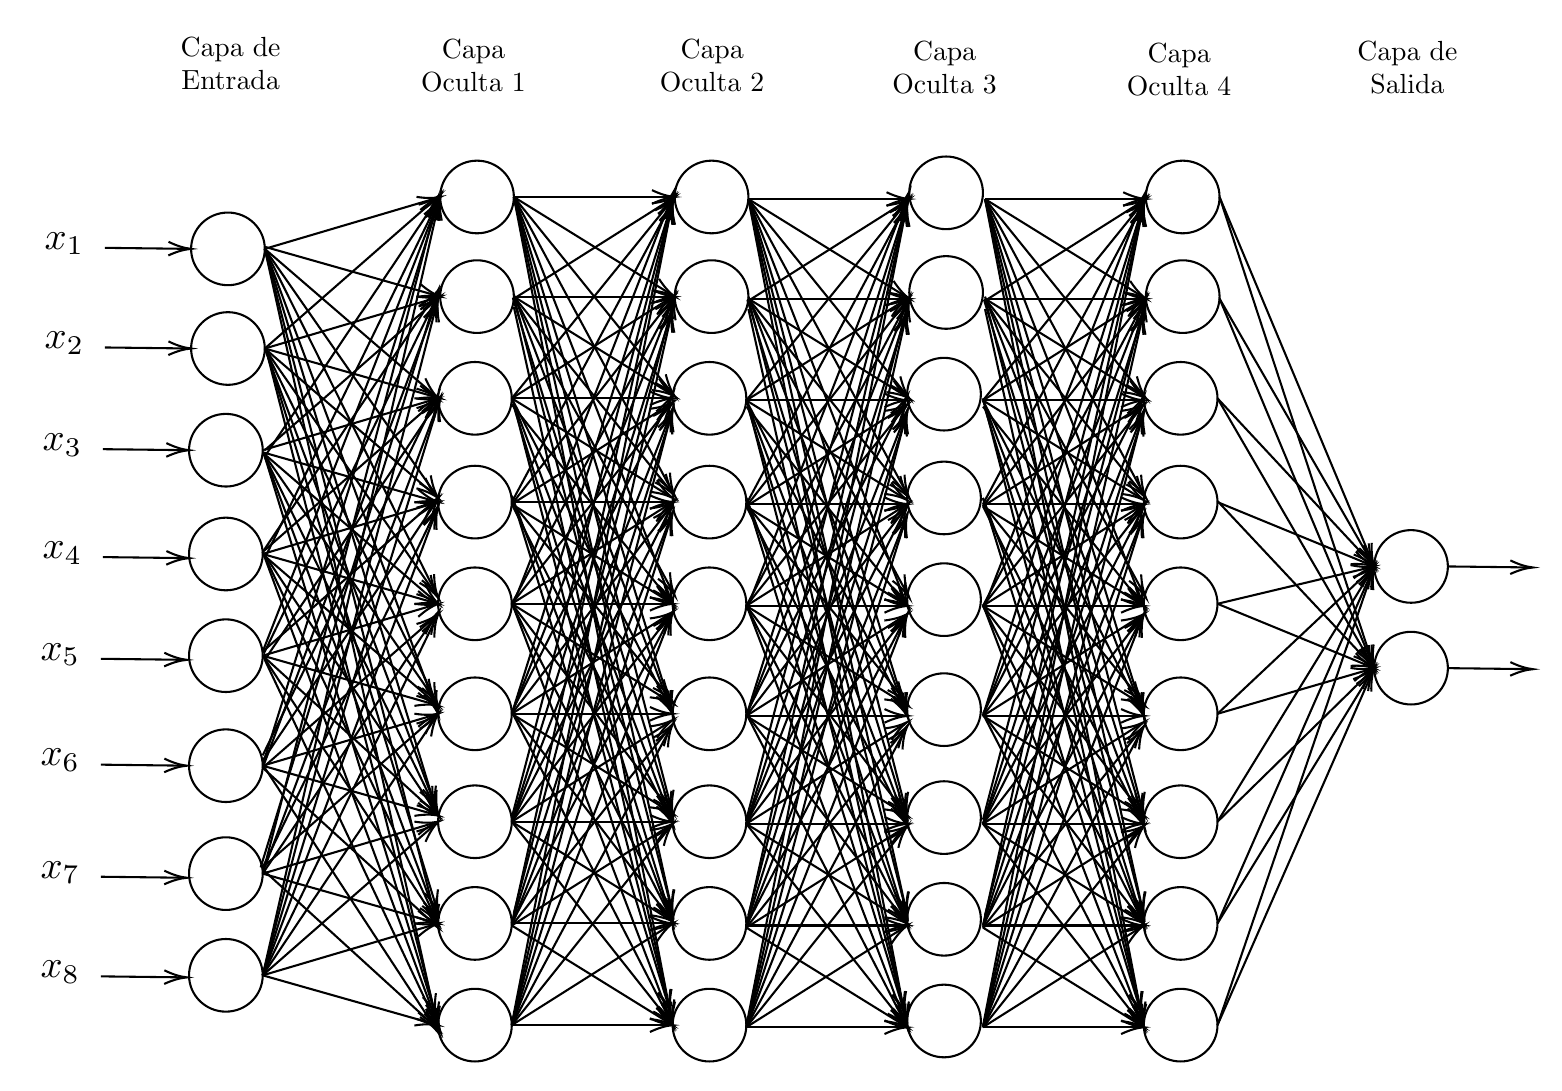
\begin{tikzpicture}[x=0.75pt,y=0.75pt,yscale=-1,xscale=1]
%uncomment if require: \path (0,815); %set diagram left start at 0, and has height of 815

%Flowchart: Connector [id:dp16560786832205587] 
\draw   (170,124.5) .. controls (170,114.84) and (177.95,107) .. (187.75,107) .. controls (197.55,107) and (205.5,114.84) .. (205.5,124.5) .. controls (205.5,134.16) and (197.55,142) .. (187.75,142) .. controls (177.95,142) and (170,134.16) .. (170,124.5) -- cycle ;
%Flowchart: Connector [id:dp7173746250705452] 
\draw   (169,271.5) .. controls (169,261.84) and (176.95,254) .. (186.75,254) .. controls (196.55,254) and (204.5,261.84) .. (204.5,271.5) .. controls (204.5,281.16) and (196.55,289) .. (186.75,289) .. controls (176.95,289) and (169,281.16) .. (169,271.5) -- cycle ;
%Flowchart: Connector [id:dp9121896584469231] 
\draw   (169,221.5) .. controls (169,211.84) and (176.95,204) .. (186.75,204) .. controls (196.55,204) and (204.5,211.84) .. (204.5,221.5) .. controls (204.5,231.16) and (196.55,239) .. (186.75,239) .. controls (176.95,239) and (169,231.16) .. (169,221.5) -- cycle ;
%Flowchart: Connector [id:dp11455401577900037] 
\draw   (170,172.5) .. controls (170,162.84) and (177.95,155) .. (187.75,155) .. controls (197.55,155) and (205.5,162.84) .. (205.5,172.5) .. controls (205.5,182.16) and (197.55,190) .. (187.75,190) .. controls (177.95,190) and (170,182.16) .. (170,172.5) -- cycle ;
%Flowchart: Connector [id:dp5025307987906783] 
\draw   (169,320.5) .. controls (169,310.84) and (176.95,303) .. (186.75,303) .. controls (196.55,303) and (204.5,310.84) .. (204.5,320.5) .. controls (204.5,330.16) and (196.55,338) .. (186.75,338) .. controls (176.95,338) and (169,330.16) .. (169,320.5) -- cycle ;
%Flowchart: Connector [id:dp9001617065749445] 
\draw   (169,474.5) .. controls (169,464.84) and (176.95,457) .. (186.75,457) .. controls (196.55,457) and (204.5,464.84) .. (204.5,474.5) .. controls (204.5,484.16) and (196.55,492) .. (186.75,492) .. controls (176.95,492) and (169,484.16) .. (169,474.5) -- cycle ;
%Flowchart: Connector [id:dp17125750369438741] 
\draw   (169,425.5) .. controls (169,415.84) and (176.95,408) .. (186.75,408) .. controls (196.55,408) and (204.5,415.84) .. (204.5,425.5) .. controls (204.5,435.16) and (196.55,443) .. (186.75,443) .. controls (176.95,443) and (169,435.16) .. (169,425.5) -- cycle ;
%Flowchart: Connector [id:dp5164677567551855] 
\draw   (169,373.5) .. controls (169,363.84) and (176.95,356) .. (186.75,356) .. controls (196.55,356) and (204.5,363.84) .. (204.5,373.5) .. controls (204.5,383.16) and (196.55,391) .. (186.75,391) .. controls (176.95,391) and (169,383.16) .. (169,373.5) -- cycle ;
%Flowchart: Connector [id:dp8699410608361591] 
\draw   (290,99.5) .. controls (290,89.84) and (297.95,82) .. (307.75,82) .. controls (317.55,82) and (325.5,89.84) .. (325.5,99.5) .. controls (325.5,109.16) and (317.55,117) .. (307.75,117) .. controls (297.95,117) and (290,109.16) .. (290,99.5) -- cycle ;
%Flowchart: Connector [id:dp8450754562961025] 
\draw   (289,246.5) .. controls (289,236.84) and (296.95,229) .. (306.75,229) .. controls (316.55,229) and (324.5,236.84) .. (324.5,246.5) .. controls (324.5,256.16) and (316.55,264) .. (306.75,264) .. controls (296.95,264) and (289,256.16) .. (289,246.5) -- cycle ;
%Flowchart: Connector [id:dp5051421192065264] 
\draw   (289,196.5) .. controls (289,186.84) and (296.95,179) .. (306.75,179) .. controls (316.55,179) and (324.5,186.84) .. (324.5,196.5) .. controls (324.5,206.16) and (316.55,214) .. (306.75,214) .. controls (296.95,214) and (289,206.16) .. (289,196.5) -- cycle ;
%Flowchart: Connector [id:dp9272105383410812] 
\draw   (290,147.5) .. controls (290,137.84) and (297.95,130) .. (307.75,130) .. controls (317.55,130) and (325.5,137.84) .. (325.5,147.5) .. controls (325.5,157.16) and (317.55,165) .. (307.75,165) .. controls (297.95,165) and (290,157.16) .. (290,147.5) -- cycle ;
%Flowchart: Connector [id:dp7274961823889059] 
\draw   (289,295.5) .. controls (289,285.84) and (296.95,278) .. (306.75,278) .. controls (316.55,278) and (324.5,285.84) .. (324.5,295.5) .. controls (324.5,305.16) and (316.55,313) .. (306.75,313) .. controls (296.95,313) and (289,305.16) .. (289,295.5) -- cycle ;
%Flowchart: Connector [id:dp05345032039364994] 
\draw   (289,449.5) .. controls (289,439.84) and (296.95,432) .. (306.75,432) .. controls (316.55,432) and (324.5,439.84) .. (324.5,449.5) .. controls (324.5,459.16) and (316.55,467) .. (306.75,467) .. controls (296.95,467) and (289,459.16) .. (289,449.5) -- cycle ;
%Flowchart: Connector [id:dp9949647071456152] 
\draw   (289,400.5) .. controls (289,390.84) and (296.95,383) .. (306.75,383) .. controls (316.55,383) and (324.5,390.84) .. (324.5,400.5) .. controls (324.5,410.16) and (316.55,418) .. (306.75,418) .. controls (296.95,418) and (289,410.16) .. (289,400.5) -- cycle ;
%Flowchart: Connector [id:dp16268028385890743] 
\draw   (289,348.5) .. controls (289,338.84) and (296.95,331) .. (306.75,331) .. controls (316.55,331) and (324.5,338.84) .. (324.5,348.5) .. controls (324.5,358.16) and (316.55,366) .. (306.75,366) .. controls (296.95,366) and (289,358.16) .. (289,348.5) -- cycle ;
%Flowchart: Connector [id:dp9227220806953265] 
\draw   (289,498.5) .. controls (289,488.84) and (296.95,481) .. (306.75,481) .. controls (316.55,481) and (324.5,488.84) .. (324.5,498.5) .. controls (324.5,508.16) and (316.55,516) .. (306.75,516) .. controls (296.95,516) and (289,508.16) .. (289,498.5) -- cycle ;
%Flowchart: Connector [id:dp9736557080850569] 
\draw   (403,99.5) .. controls (403,89.84) and (410.95,82) .. (420.75,82) .. controls (430.55,82) and (438.5,89.84) .. (438.5,99.5) .. controls (438.5,109.16) and (430.55,117) .. (420.75,117) .. controls (410.95,117) and (403,109.16) .. (403,99.5) -- cycle ;
%Flowchart: Connector [id:dp39081687422878575] 
\draw   (402,246.5) .. controls (402,236.84) and (409.95,229) .. (419.75,229) .. controls (429.55,229) and (437.5,236.84) .. (437.5,246.5) .. controls (437.5,256.16) and (429.55,264) .. (419.75,264) .. controls (409.95,264) and (402,256.16) .. (402,246.5) -- cycle ;
%Flowchart: Connector [id:dp3641680498880344] 
\draw   (402,196.5) .. controls (402,186.84) and (409.95,179) .. (419.75,179) .. controls (429.55,179) and (437.5,186.84) .. (437.5,196.5) .. controls (437.5,206.16) and (429.55,214) .. (419.75,214) .. controls (409.95,214) and (402,206.16) .. (402,196.5) -- cycle ;
%Flowchart: Connector [id:dp5434574012242319] 
\draw   (403,147.5) .. controls (403,137.84) and (410.95,130) .. (420.75,130) .. controls (430.55,130) and (438.5,137.84) .. (438.5,147.5) .. controls (438.5,157.16) and (430.55,165) .. (420.75,165) .. controls (410.95,165) and (403,157.16) .. (403,147.5) -- cycle ;
%Flowchart: Connector [id:dp22919386292790211] 
\draw   (402,295.5) .. controls (402,285.84) and (409.95,278) .. (419.75,278) .. controls (429.55,278) and (437.5,285.84) .. (437.5,295.5) .. controls (437.5,305.16) and (429.55,313) .. (419.75,313) .. controls (409.95,313) and (402,305.16) .. (402,295.5) -- cycle ;
%Flowchart: Connector [id:dp27996688198185327] 
\draw   (402,449.5) .. controls (402,439.84) and (409.95,432) .. (419.75,432) .. controls (429.55,432) and (437.5,439.84) .. (437.5,449.5) .. controls (437.5,459.16) and (429.55,467) .. (419.75,467) .. controls (409.95,467) and (402,459.16) .. (402,449.5) -- cycle ;
%Flowchart: Connector [id:dp651749202654733] 
\draw   (402,400.5) .. controls (402,390.84) and (409.95,383) .. (419.75,383) .. controls (429.55,383) and (437.5,390.84) .. (437.5,400.5) .. controls (437.5,410.16) and (429.55,418) .. (419.75,418) .. controls (409.95,418) and (402,410.16) .. (402,400.5) -- cycle ;
%Flowchart: Connector [id:dp9472207745433454] 
\draw   (402,348.5) .. controls (402,338.84) and (409.95,331) .. (419.75,331) .. controls (429.55,331) and (437.5,338.84) .. (437.5,348.5) .. controls (437.5,358.16) and (429.55,366) .. (419.75,366) .. controls (409.95,366) and (402,358.16) .. (402,348.5) -- cycle ;
%Flowchart: Connector [id:dp4324076862378343] 
\draw   (402,498.5) .. controls (402,488.84) and (409.95,481) .. (419.75,481) .. controls (429.55,481) and (437.5,488.84) .. (437.5,498.5) .. controls (437.5,508.16) and (429.55,516) .. (419.75,516) .. controls (409.95,516) and (402,508.16) .. (402,498.5) -- cycle ;
%Flowchart: Connector [id:dp6627691577686355] 
\draw   (516,97.5) .. controls (516,87.84) and (523.95,80) .. (533.75,80) .. controls (543.55,80) and (551.5,87.84) .. (551.5,97.5) .. controls (551.5,107.16) and (543.55,115) .. (533.75,115) .. controls (523.95,115) and (516,107.16) .. (516,97.5) -- cycle ;
%Flowchart: Connector [id:dp02572592612155966] 
\draw   (515,244.5) .. controls (515,234.84) and (522.95,227) .. (532.75,227) .. controls (542.55,227) and (550.5,234.84) .. (550.5,244.5) .. controls (550.5,254.16) and (542.55,262) .. (532.75,262) .. controls (522.95,262) and (515,254.16) .. (515,244.5) -- cycle ;
%Flowchart: Connector [id:dp7087150813151666] 
\draw   (515,194.5) .. controls (515,184.84) and (522.95,177) .. (532.75,177) .. controls (542.55,177) and (550.5,184.84) .. (550.5,194.5) .. controls (550.5,204.16) and (542.55,212) .. (532.75,212) .. controls (522.95,212) and (515,204.16) .. (515,194.5) -- cycle ;
%Flowchart: Connector [id:dp6340767640386636] 
\draw   (516,145.5) .. controls (516,135.84) and (523.95,128) .. (533.75,128) .. controls (543.55,128) and (551.5,135.84) .. (551.5,145.5) .. controls (551.5,155.16) and (543.55,163) .. (533.75,163) .. controls (523.95,163) and (516,155.16) .. (516,145.5) -- cycle ;
%Flowchart: Connector [id:dp9395698096272754] 
\draw   (515,293.5) .. controls (515,283.84) and (522.95,276) .. (532.75,276) .. controls (542.55,276) and (550.5,283.84) .. (550.5,293.5) .. controls (550.5,303.16) and (542.55,311) .. (532.75,311) .. controls (522.95,311) and (515,303.16) .. (515,293.5) -- cycle ;
%Flowchart: Connector [id:dp7610216163012721] 
\draw   (515,447.5) .. controls (515,437.84) and (522.95,430) .. (532.75,430) .. controls (542.55,430) and (550.5,437.84) .. (550.5,447.5) .. controls (550.5,457.16) and (542.55,465) .. (532.75,465) .. controls (522.95,465) and (515,457.16) .. (515,447.5) -- cycle ;
%Flowchart: Connector [id:dp9921400919388911] 
\draw   (515,398.5) .. controls (515,388.84) and (522.95,381) .. (532.75,381) .. controls (542.55,381) and (550.5,388.84) .. (550.5,398.5) .. controls (550.5,408.16) and (542.55,416) .. (532.75,416) .. controls (522.95,416) and (515,408.16) .. (515,398.5) -- cycle ;
%Flowchart: Connector [id:dp25669993219598664] 
\draw   (515,346.5) .. controls (515,336.84) and (522.95,329) .. (532.75,329) .. controls (542.55,329) and (550.5,336.84) .. (550.5,346.5) .. controls (550.5,356.16) and (542.55,364) .. (532.75,364) .. controls (522.95,364) and (515,356.16) .. (515,346.5) -- cycle ;
%Flowchart: Connector [id:dp46222469436683067] 
\draw   (515,496.5) .. controls (515,486.84) and (522.95,479) .. (532.75,479) .. controls (542.55,479) and (550.5,486.84) .. (550.5,496.5) .. controls (550.5,506.16) and (542.55,514) .. (532.75,514) .. controls (522.95,514) and (515,506.16) .. (515,496.5) -- cycle ;
%Flowchart: Connector [id:dp025086483746098898] 
\draw   (630,99.5) .. controls (630,89.84) and (637.95,82) .. (647.75,82) .. controls (657.55,82) and (665.5,89.84) .. (665.5,99.5) .. controls (665.5,109.16) and (657.55,117) .. (647.75,117) .. controls (637.95,117) and (630,109.16) .. (630,99.5) -- cycle ;
%Flowchart: Connector [id:dp9163522668741138] 
\draw   (629,246.5) .. controls (629,236.84) and (636.95,229) .. (646.75,229) .. controls (656.55,229) and (664.5,236.84) .. (664.5,246.5) .. controls (664.5,256.16) and (656.55,264) .. (646.75,264) .. controls (636.95,264) and (629,256.16) .. (629,246.5) -- cycle ;
%Flowchart: Connector [id:dp199831354937975] 
\draw   (629,196.5) .. controls (629,186.84) and (636.95,179) .. (646.75,179) .. controls (656.55,179) and (664.5,186.84) .. (664.5,196.5) .. controls (664.5,206.16) and (656.55,214) .. (646.75,214) .. controls (636.95,214) and (629,206.16) .. (629,196.5) -- cycle ;
%Flowchart: Connector [id:dp2437266960320149] 
\draw   (630,147.5) .. controls (630,137.84) and (637.95,130) .. (647.75,130) .. controls (657.55,130) and (665.5,137.84) .. (665.5,147.5) .. controls (665.5,157.16) and (657.55,165) .. (647.75,165) .. controls (637.95,165) and (630,157.16) .. (630,147.5) -- cycle ;
%Flowchart: Connector [id:dp664586587609465] 
\draw   (629,295.5) .. controls (629,285.84) and (636.95,278) .. (646.75,278) .. controls (656.55,278) and (664.5,285.84) .. (664.5,295.5) .. controls (664.5,305.16) and (656.55,313) .. (646.75,313) .. controls (636.95,313) and (629,305.16) .. (629,295.5) -- cycle ;
%Flowchart: Connector [id:dp8428547725140251] 
\draw   (629,449.5) .. controls (629,439.84) and (636.95,432) .. (646.75,432) .. controls (656.55,432) and (664.5,439.84) .. (664.5,449.5) .. controls (664.5,459.16) and (656.55,467) .. (646.75,467) .. controls (636.95,467) and (629,459.16) .. (629,449.5) -- cycle ;
%Flowchart: Connector [id:dp03338516073217779] 
\draw   (629,400.5) .. controls (629,390.84) and (636.95,383) .. (646.75,383) .. controls (656.55,383) and (664.5,390.84) .. (664.5,400.5) .. controls (664.5,410.16) and (656.55,418) .. (646.75,418) .. controls (636.95,418) and (629,410.16) .. (629,400.5) -- cycle ;
%Flowchart: Connector [id:dp7296113676407779] 
\draw   (629,348.5) .. controls (629,338.84) and (636.95,331) .. (646.75,331) .. controls (656.55,331) and (664.5,338.84) .. (664.5,348.5) .. controls (664.5,358.16) and (656.55,366) .. (646.75,366) .. controls (636.95,366) and (629,358.16) .. (629,348.5) -- cycle ;
%Flowchart: Connector [id:dp5867156683549041] 
\draw   (629,498.5) .. controls (629,488.84) and (636.95,481) .. (646.75,481) .. controls (656.55,481) and (664.5,488.84) .. (664.5,498.5) .. controls (664.5,508.16) and (656.55,516) .. (646.75,516) .. controls (636.95,516) and (629,508.16) .. (629,498.5) -- cycle ;
%Flowchart: Connector [id:dp035759492726770814] 
\draw   (740,277.5) .. controls (740,267.84) and (747.95,260) .. (757.75,260) .. controls (767.55,260) and (775.5,267.84) .. (775.5,277.5) .. controls (775.5,287.16) and (767.55,295) .. (757.75,295) .. controls (747.95,295) and (740,287.16) .. (740,277.5) -- cycle ;
%Flowchart: Connector [id:dp18374339909919435] 
\draw   (740,326.5) .. controls (740,316.84) and (747.95,309) .. (757.75,309) .. controls (767.55,309) and (775.5,316.84) .. (775.5,326.5) .. controls (775.5,336.16) and (767.55,344) .. (757.75,344) .. controls (747.95,344) and (740,336.16) .. (740,326.5) -- cycle ;
%Straight Lines [id:da9586956729956472] 
\draw    (205.5,124.5) -- (288.08,100.07) ;
\draw [shift={(290,99.5)}, rotate = 523.52] [color={rgb, 255:red, 0; green, 0; blue, 0 }  ][line width=0.75]    (10.93,-3.29) .. controls (6.95,-1.4) and (3.31,-0.3) .. (0,0) .. controls (3.31,0.3) and (6.95,1.4) .. (10.93,3.29)   ;

%Straight Lines [id:da0977247729203864] 
\draw    (205.5,172.5) -- (288.08,148.07) ;
\draw [shift={(290,147.5)}, rotate = 523.52] [color={rgb, 255:red, 0; green, 0; blue, 0 }  ][line width=0.75]    (10.93,-3.29) .. controls (6.95,-1.4) and (3.31,-0.3) .. (0,0) .. controls (3.31,0.3) and (6.95,1.4) .. (10.93,3.29)   ;

%Straight Lines [id:da12300871068905828] 
\draw    (204.5,221.5) -- (287.08,197.07) ;
\draw [shift={(289,196.5)}, rotate = 523.52] [color={rgb, 255:red, 0; green, 0; blue, 0 }  ][line width=0.75]    (10.93,-3.29) .. controls (6.95,-1.4) and (3.31,-0.3) .. (0,0) .. controls (3.31,0.3) and (6.95,1.4) .. (10.93,3.29)   ;

%Straight Lines [id:da8590282898076349] 
\draw    (204.5,271.5) -- (287.08,247.07) ;
\draw [shift={(289,246.5)}, rotate = 523.52] [color={rgb, 255:red, 0; green, 0; blue, 0 }  ][line width=0.75]    (10.93,-3.29) .. controls (6.95,-1.4) and (3.31,-0.3) .. (0,0) .. controls (3.31,0.3) and (6.95,1.4) .. (10.93,3.29)   ;

%Straight Lines [id:da9466521849421138] 
\draw    (204.5,320.5) -- (287.08,296.07) ;
\draw [shift={(289,295.5)}, rotate = 523.52] [color={rgb, 255:red, 0; green, 0; blue, 0 }  ][line width=0.75]    (10.93,-3.29) .. controls (6.95,-1.4) and (3.31,-0.3) .. (0,0) .. controls (3.31,0.3) and (6.95,1.4) .. (10.93,3.29)   ;

%Straight Lines [id:da9538137596119758] 
\draw    (204.5,373.5) -- (287.08,349.07) ;
\draw [shift={(289,348.5)}, rotate = 523.52] [color={rgb, 255:red, 0; green, 0; blue, 0 }  ][line width=0.75]    (10.93,-3.29) .. controls (6.95,-1.4) and (3.31,-0.3) .. (0,0) .. controls (3.31,0.3) and (6.95,1.4) .. (10.93,3.29)   ;

%Straight Lines [id:da45752309491080034] 
\draw    (204.5,425.5) -- (287.08,401.07) ;
\draw [shift={(289,400.5)}, rotate = 523.52] [color={rgb, 255:red, 0; green, 0; blue, 0 }  ][line width=0.75]    (10.93,-3.29) .. controls (6.95,-1.4) and (3.31,-0.3) .. (0,0) .. controls (3.31,0.3) and (6.95,1.4) .. (10.93,3.29)   ;

%Straight Lines [id:da8992659646731549] 
\draw    (204.5,474.5) -- (287.08,450.07) ;
\draw [shift={(289,449.5)}, rotate = 523.52] [color={rgb, 255:red, 0; green, 0; blue, 0 }  ][line width=0.75]    (10.93,-3.29) .. controls (6.95,-1.4) and (3.31,-0.3) .. (0,0) .. controls (3.31,0.3) and (6.95,1.4) .. (10.93,3.29)   ;

%Straight Lines [id:da2506301756766518] 
\draw    (204.5,474.5) -- (287.08,497.95) ;
\draw [shift={(289,498.5)}, rotate = 195.86] [color={rgb, 255:red, 0; green, 0; blue, 0 }  ][line width=0.75]    (10.93,-3.29) .. controls (6.95,-1.4) and (3.31,-0.3) .. (0,0) .. controls (3.31,0.3) and (6.95,1.4) .. (10.93,3.29)   ;

%Straight Lines [id:da18877659342428144] 
\draw    (204.5,425.5) -- (287.08,448.95) ;
\draw [shift={(289,449.5)}, rotate = 195.86] [color={rgb, 255:red, 0; green, 0; blue, 0 }  ][line width=0.75]    (10.93,-3.29) .. controls (6.95,-1.4) and (3.31,-0.3) .. (0,0) .. controls (3.31,0.3) and (6.95,1.4) .. (10.93,3.29)   ;

%Straight Lines [id:da7190090533273531] 
\draw    (204.5,373.5) -- (287.08,396.95) ;
\draw [shift={(289,397.5)}, rotate = 195.86] [color={rgb, 255:red, 0; green, 0; blue, 0 }  ][line width=0.75]    (10.93,-3.29) .. controls (6.95,-1.4) and (3.31,-0.3) .. (0,0) .. controls (3.31,0.3) and (6.95,1.4) .. (10.93,3.29)   ;

%Straight Lines [id:da13502320247798016] 
\draw    (204.5,320.5) -- (287.08,343.95) ;
\draw [shift={(289,344.5)}, rotate = 195.86] [color={rgb, 255:red, 0; green, 0; blue, 0 }  ][line width=0.75]    (10.93,-3.29) .. controls (6.95,-1.4) and (3.31,-0.3) .. (0,0) .. controls (3.31,0.3) and (6.95,1.4) .. (10.93,3.29)   ;

%Straight Lines [id:da7949562195729276] 
\draw    (204.5,271.5) -- (287.08,294.95) ;
\draw [shift={(289,295.5)}, rotate = 195.86] [color={rgb, 255:red, 0; green, 0; blue, 0 }  ][line width=0.75]    (10.93,-3.29) .. controls (6.95,-1.4) and (3.31,-0.3) .. (0,0) .. controls (3.31,0.3) and (6.95,1.4) .. (10.93,3.29)   ;

%Straight Lines [id:da7503826016354034] 
\draw    (204.5,222.5) -- (287.08,245.95) ;
\draw [shift={(289,246.5)}, rotate = 195.86] [color={rgb, 255:red, 0; green, 0; blue, 0 }  ][line width=0.75]    (10.93,-3.29) .. controls (6.95,-1.4) and (3.31,-0.3) .. (0,0) .. controls (3.31,0.3) and (6.95,1.4) .. (10.93,3.29)   ;

%Straight Lines [id:da9545679852436817] 
\draw    (205.5,172.5) -- (288.08,195.95) ;
\draw [shift={(290,196.5)}, rotate = 195.86] [color={rgb, 255:red, 0; green, 0; blue, 0 }  ][line width=0.75]    (10.93,-3.29) .. controls (6.95,-1.4) and (3.31,-0.3) .. (0,0) .. controls (3.31,0.3) and (6.95,1.4) .. (10.93,3.29)   ;

%Straight Lines [id:da15732159593119666] 
\draw    (205.5,123.5) -- (288.08,146.95) ;
\draw [shift={(290,147.5)}, rotate = 195.86] [color={rgb, 255:red, 0; green, 0; blue, 0 }  ][line width=0.75]    (10.93,-3.29) .. controls (6.95,-1.4) and (3.31,-0.3) .. (0,0) .. controls (3.31,0.3) and (6.95,1.4) .. (10.93,3.29)   ;

%Straight Lines [id:da6302921654092268] 
\draw    (205.5,124.5) -- (287.49,195.19) ;
\draw [shift={(289,196.5)}, rotate = 220.77] [color={rgb, 255:red, 0; green, 0; blue, 0 }  ][line width=0.75]    (10.93,-3.29) .. controls (6.95,-1.4) and (3.31,-0.3) .. (0,0) .. controls (3.31,0.3) and (6.95,1.4) .. (10.93,3.29)   ;

%Straight Lines [id:da6254331993045943] 
\draw    (205.5,172.5) -- (287.49,243.19) ;
\draw [shift={(289,244.5)}, rotate = 220.77] [color={rgb, 255:red, 0; green, 0; blue, 0 }  ][line width=0.75]    (10.93,-3.29) .. controls (6.95,-1.4) and (3.31,-0.3) .. (0,0) .. controls (3.31,0.3) and (6.95,1.4) .. (10.93,3.29)   ;

%Straight Lines [id:da3704783366173454] 
\draw    (205.5,223.5) -- (287.49,294.19) ;
\draw [shift={(289,295.5)}, rotate = 220.77] [color={rgb, 255:red, 0; green, 0; blue, 0 }  ][line width=0.75]    (10.93,-3.29) .. controls (6.95,-1.4) and (3.31,-0.3) .. (0,0) .. controls (3.31,0.3) and (6.95,1.4) .. (10.93,3.29)   ;

%Straight Lines [id:da48243047605882927] 
\draw    (205.5,272.5) -- (287.49,343.19) ;
\draw [shift={(289,344.5)}, rotate = 220.77] [color={rgb, 255:red, 0; green, 0; blue, 0 }  ][line width=0.75]    (10.93,-3.29) .. controls (6.95,-1.4) and (3.31,-0.3) .. (0,0) .. controls (3.31,0.3) and (6.95,1.4) .. (10.93,3.29)   ;

%Straight Lines [id:da8955499843073155] 
\draw    (204.5,320.5) -- (287.52,396.15) ;
\draw [shift={(289,397.5)}, rotate = 222.34] [color={rgb, 255:red, 0; green, 0; blue, 0 }  ][line width=0.75]    (10.93,-3.29) .. controls (6.95,-1.4) and (3.31,-0.3) .. (0,0) .. controls (3.31,0.3) and (6.95,1.4) .. (10.93,3.29)   ;

%Straight Lines [id:da8065776986048846] 
\draw    (204.5,374.5) -- (287.52,450.15) ;
\draw [shift={(289,451.5)}, rotate = 222.34] [color={rgb, 255:red, 0; green, 0; blue, 0 }  ][line width=0.75]    (10.93,-3.29) .. controls (6.95,-1.4) and (3.31,-0.3) .. (0,0) .. controls (3.31,0.3) and (6.95,1.4) .. (10.93,3.29)   ;

%Straight Lines [id:da1338711011126129] 
\draw    (204.5,423.5) -- (287.52,499.15) ;
\draw [shift={(289,500.5)}, rotate = 222.34] [color={rgb, 255:red, 0; green, 0; blue, 0 }  ][line width=0.75]    (10.93,-3.29) .. controls (6.95,-1.4) and (3.31,-0.3) .. (0,0) .. controls (3.31,0.3) and (6.95,1.4) .. (10.93,3.29)   ;

%Straight Lines [id:da08339712060915827] 
\draw    (204.5,474.5) -- (287.5,401.82) ;
\draw [shift={(289,400.5)}, rotate = 498.79] [color={rgb, 255:red, 0; green, 0; blue, 0 }  ][line width=0.75]    (10.93,-3.29) .. controls (6.95,-1.4) and (3.31,-0.3) .. (0,0) .. controls (3.31,0.3) and (6.95,1.4) .. (10.93,3.29)   ;

%Straight Lines [id:da5405393078384249] 
\draw    (204.5,422.5) -- (287.5,349.82) ;
\draw [shift={(289,348.5)}, rotate = 498.79] [color={rgb, 255:red, 0; green, 0; blue, 0 }  ][line width=0.75]    (10.93,-3.29) .. controls (6.95,-1.4) and (3.31,-0.3) .. (0,0) .. controls (3.31,0.3) and (6.95,1.4) .. (10.93,3.29)   ;

%Straight Lines [id:da011274598498959731] 
\draw    (204.5,374.5) -- (287.5,301.82) ;
\draw [shift={(289,300.5)}, rotate = 498.79] [color={rgb, 255:red, 0; green, 0; blue, 0 }  ][line width=0.75]    (10.93,-3.29) .. controls (6.95,-1.4) and (3.31,-0.3) .. (0,0) .. controls (3.31,0.3) and (6.95,1.4) .. (10.93,3.29)   ;

%Straight Lines [id:da6020385780831415] 
\draw    (204.5,318.5) -- (287.5,245.82) ;
\draw [shift={(289,244.5)}, rotate = 498.79] [color={rgb, 255:red, 0; green, 0; blue, 0 }  ][line width=0.75]    (10.93,-3.29) .. controls (6.95,-1.4) and (3.31,-0.3) .. (0,0) .. controls (3.31,0.3) and (6.95,1.4) .. (10.93,3.29)   ;

%Straight Lines [id:da1387063960287005] 
\draw    (204.5,270.5) -- (287.5,197.82) ;
\draw [shift={(289,196.5)}, rotate = 498.79] [color={rgb, 255:red, 0; green, 0; blue, 0 }  ][line width=0.75]    (10.93,-3.29) .. controls (6.95,-1.4) and (3.31,-0.3) .. (0,0) .. controls (3.31,0.3) and (6.95,1.4) .. (10.93,3.29)   ;

%Straight Lines [id:da790054862269482] 
\draw    (205.5,221.5) -- (288.5,148.82) ;
\draw [shift={(290,147.5)}, rotate = 498.79] [color={rgb, 255:red, 0; green, 0; blue, 0 }  ][line width=0.75]    (10.93,-3.29) .. controls (6.95,-1.4) and (3.31,-0.3) .. (0,0) .. controls (3.31,0.3) and (6.95,1.4) .. (10.93,3.29)   ;

%Straight Lines [id:da28998972905081044] 
\draw    (205.5,172.5) -- (288.5,99.82) ;
\draw [shift={(290,98.5)}, rotate = 498.79] [color={rgb, 255:red, 0; green, 0; blue, 0 }  ][line width=0.75]    (10.93,-3.29) .. controls (6.95,-1.4) and (3.31,-0.3) .. (0,0) .. controls (3.31,0.3) and (6.95,1.4) .. (10.93,3.29)   ;

%Straight Lines [id:da5101104296010823] 
\draw    (205.5,124.5) -- (287.86,242.86) ;
\draw [shift={(289,244.5)}, rotate = 235.17000000000002] [color={rgb, 255:red, 0; green, 0; blue, 0 }  ][line width=0.75]    (10.93,-3.29) .. controls (6.95,-1.4) and (3.31,-0.3) .. (0,0) .. controls (3.31,0.3) and (6.95,1.4) .. (10.93,3.29)   ;

%Straight Lines [id:da9488543308531325] 
\draw    (205.5,172.5) -- (287.86,290.86) ;
\draw [shift={(289,292.5)}, rotate = 235.17000000000002] [color={rgb, 255:red, 0; green, 0; blue, 0 }  ][line width=0.75]    (10.93,-3.29) .. controls (6.95,-1.4) and (3.31,-0.3) .. (0,0) .. controls (3.31,0.3) and (6.95,1.4) .. (10.93,3.29)   ;

%Straight Lines [id:da7854731760655506] 
\draw    (204.5,222.5) -- (286.86,340.86) ;
\draw [shift={(288,342.5)}, rotate = 235.17000000000002] [color={rgb, 255:red, 0; green, 0; blue, 0 }  ][line width=0.75]    (10.93,-3.29) .. controls (6.95,-1.4) and (3.31,-0.3) .. (0,0) .. controls (3.31,0.3) and (6.95,1.4) .. (10.93,3.29)   ;

%Straight Lines [id:da8090153287019111] 
\draw    (204.5,270.5) -- (287.89,395.83) ;
\draw [shift={(289,397.5)}, rotate = 236.36] [color={rgb, 255:red, 0; green, 0; blue, 0 }  ][line width=0.75]    (10.93,-3.29) .. controls (6.95,-1.4) and (3.31,-0.3) .. (0,0) .. controls (3.31,0.3) and (6.95,1.4) .. (10.93,3.29)   ;

%Straight Lines [id:da9915951156386728] 
\draw    (204.5,320.5) -- (287.9,447.83) ;
\draw [shift={(289,449.5)}, rotate = 236.77] [color={rgb, 255:red, 0; green, 0; blue, 0 }  ][line width=0.75]    (10.93,-3.29) .. controls (6.95,-1.4) and (3.31,-0.3) .. (0,0) .. controls (3.31,0.3) and (6.95,1.4) .. (10.93,3.29)   ;

%Straight Lines [id:da4583459539022623] 
\draw    (204.5,373) -- (287.9,500.33) ;
\draw [shift={(289,502)}, rotate = 236.77] [color={rgb, 255:red, 0; green, 0; blue, 0 }  ][line width=0.75]    (10.93,-3.29) .. controls (6.95,-1.4) and (3.31,-0.3) .. (0,0) .. controls (3.31,0.3) and (6.95,1.4) .. (10.93,3.29)   ;

%Straight Lines [id:da21777412102717897] 
\draw    (204.5,474.5) -- (287.89,350.16) ;
\draw [shift={(289,348.5)}, rotate = 483.85] [color={rgb, 255:red, 0; green, 0; blue, 0 }  ][line width=0.75]    (10.93,-3.29) .. controls (6.95,-1.4) and (3.31,-0.3) .. (0,0) .. controls (3.31,0.3) and (6.95,1.4) .. (10.93,3.29)   ;

%Straight Lines [id:da9172582440884776] 
\draw    (204.5,425.5) -- (287.89,301.16) ;
\draw [shift={(289,299.5)}, rotate = 483.85] [color={rgb, 255:red, 0; green, 0; blue, 0 }  ][line width=0.75]    (10.93,-3.29) .. controls (6.95,-1.4) and (3.31,-0.3) .. (0,0) .. controls (3.31,0.3) and (6.95,1.4) .. (10.93,3.29)   ;

%Straight Lines [id:da9823806685957189] 
\draw    (204.5,371) -- (287.89,246.66) ;
\draw [shift={(289,245)}, rotate = 483.85] [color={rgb, 255:red, 0; green, 0; blue, 0 }  ][line width=0.75]    (10.93,-3.29) .. controls (6.95,-1.4) and (3.31,-0.3) .. (0,0) .. controls (3.31,0.3) and (6.95,1.4) .. (10.93,3.29)   ;

%Straight Lines [id:da026880414159362598] 
\draw    (205.5,322.5) -- (288.89,198.16) ;
\draw [shift={(290,196.5)}, rotate = 483.85] [color={rgb, 255:red, 0; green, 0; blue, 0 }  ][line width=0.75]    (10.93,-3.29) .. controls (6.95,-1.4) and (3.31,-0.3) .. (0,0) .. controls (3.31,0.3) and (6.95,1.4) .. (10.93,3.29)   ;

%Straight Lines [id:da37101130563675666] 
\draw    (204.5,270.5) -- (287.89,146.16) ;
\draw [shift={(289,144.5)}, rotate = 483.85] [color={rgb, 255:red, 0; green, 0; blue, 0 }  ][line width=0.75]    (10.93,-3.29) .. controls (6.95,-1.4) and (3.31,-0.3) .. (0,0) .. controls (3.31,0.3) and (6.95,1.4) .. (10.93,3.29)   ;

%Straight Lines [id:da6982102800002767] 
\draw    (205.5,224.5) -- (288.89,100.16) ;
\draw [shift={(290,98.5)}, rotate = 483.85] [color={rgb, 255:red, 0; green, 0; blue, 0 }  ][line width=0.75]    (10.93,-3.29) .. controls (6.95,-1.4) and (3.31,-0.3) .. (0,0) .. controls (3.31,0.3) and (6.95,1.4) .. (10.93,3.29)   ;

%Straight Lines [id:da6559580658795142] 
\draw    (205.5,124.5) -- (288.11,290.71) ;
\draw [shift={(289,292.5)}, rotate = 243.57] [color={rgb, 255:red, 0; green, 0; blue, 0 }  ][line width=0.75]    (10.93,-3.29) .. controls (6.95,-1.4) and (3.31,-0.3) .. (0,0) .. controls (3.31,0.3) and (6.95,1.4) .. (10.93,3.29)   ;

%Straight Lines [id:da926293069155972] 
\draw    (205.5,172.5) -- (288.13,342.7) ;
\draw [shift={(289,344.5)}, rotate = 244.11] [color={rgb, 255:red, 0; green, 0; blue, 0 }  ][line width=0.75]    (10.93,-3.29) .. controls (6.95,-1.4) and (3.31,-0.3) .. (0,0) .. controls (3.31,0.3) and (6.95,1.4) .. (10.93,3.29)   ;

%Straight Lines [id:da4311095966962428] 
\draw    (204.5,222.5) -- (287.13,392.7) ;
\draw [shift={(288,394.5)}, rotate = 244.11] [color={rgb, 255:red, 0; green, 0; blue, 0 }  ][line width=0.75]    (10.93,-3.29) .. controls (6.95,-1.4) and (3.31,-0.3) .. (0,0) .. controls (3.31,0.3) and (6.95,1.4) .. (10.93,3.29)   ;

%Straight Lines [id:da16990248932248309] 
\draw    (204.5,270.5) -- (288.15,447.69) ;
\draw [shift={(289,449.5)}, rotate = 244.73000000000002] [color={rgb, 255:red, 0; green, 0; blue, 0 }  ][line width=0.75]    (10.93,-3.29) .. controls (6.95,-1.4) and (3.31,-0.3) .. (0,0) .. controls (3.31,0.3) and (6.95,1.4) .. (10.93,3.29)   ;

%Straight Lines [id:da8308042077365565] 
\draw    (205.5,322.5) -- (289.15,499.69) ;
\draw [shift={(290,501.5)}, rotate = 244.73000000000002] [color={rgb, 255:red, 0; green, 0; blue, 0 }  ][line width=0.75]    (10.93,-3.29) .. controls (6.95,-1.4) and (3.31,-0.3) .. (0,0) .. controls (3.31,0.3) and (6.95,1.4) .. (10.93,3.29)   ;

%Straight Lines [id:da06326152365467941] 
\draw    (204.5,474.5) -- (288.13,302.3) ;
\draw [shift={(289,300.5)}, rotate = 475.9] [color={rgb, 255:red, 0; green, 0; blue, 0 }  ][line width=0.75]    (10.93,-3.29) .. controls (6.95,-1.4) and (3.31,-0.3) .. (0,0) .. controls (3.31,0.3) and (6.95,1.4) .. (10.93,3.29)   ;

%Straight Lines [id:da1496273123684393] 
\draw    (204.5,422.5) -- (288.13,250.3) ;
\draw [shift={(289,248.5)}, rotate = 475.9] [color={rgb, 255:red, 0; green, 0; blue, 0 }  ][line width=0.75]    (10.93,-3.29) .. controls (6.95,-1.4) and (3.31,-0.3) .. (0,0) .. controls (3.31,0.3) and (6.95,1.4) .. (10.93,3.29)   ;

%Straight Lines [id:da060739301857917205] 
\draw    (204.5,368.5) -- (288.13,196.3) ;
\draw [shift={(289,194.5)}, rotate = 475.9] [color={rgb, 255:red, 0; green, 0; blue, 0 }  ][line width=0.75]    (10.93,-3.29) .. controls (6.95,-1.4) and (3.31,-0.3) .. (0,0) .. controls (3.31,0.3) and (6.95,1.4) .. (10.93,3.29)   ;

%Straight Lines [id:da45698957081998015] 
\draw    (205,319.5) -- (288.63,147.3) ;
\draw [shift={(289.5,145.5)}, rotate = 475.9] [color={rgb, 255:red, 0; green, 0; blue, 0 }  ][line width=0.75]    (10.93,-3.29) .. controls (6.95,-1.4) and (3.31,-0.3) .. (0,0) .. controls (3.31,0.3) and (6.95,1.4) .. (10.93,3.29)   ;

%Straight Lines [id:da4415373820513747] 
\draw    (205.5,273.5) -- (289.13,101.3) ;
\draw [shift={(290,99.5)}, rotate = 475.9] [color={rgb, 255:red, 0; green, 0; blue, 0 }  ][line width=0.75]    (10.93,-3.29) .. controls (6.95,-1.4) and (3.31,-0.3) .. (0,0) .. controls (3.31,0.3) and (6.95,1.4) .. (10.93,3.29)   ;

%Straight Lines [id:da03424673221381447] 
\draw    (205.5,124.5) -- (288.3,346.63) ;
\draw [shift={(289,348.5)}, rotate = 249.56] [color={rgb, 255:red, 0; green, 0; blue, 0 }  ][line width=0.75]    (10.93,-3.29) .. controls (6.95,-1.4) and (3.31,-0.3) .. (0,0) .. controls (3.31,0.3) and (6.95,1.4) .. (10.93,3.29)   ;

%Straight Lines [id:da3484074699401256] 
\draw    (205.5,172.5) -- (288.3,394.63) ;
\draw [shift={(289,396.5)}, rotate = 249.56] [color={rgb, 255:red, 0; green, 0; blue, 0 }  ][line width=0.75]    (10.93,-3.29) .. controls (6.95,-1.4) and (3.31,-0.3) .. (0,0) .. controls (3.31,0.3) and (6.95,1.4) .. (10.93,3.29)   ;

%Straight Lines [id:da4781222951846196] 
\draw    (205.5,224.5) -- (288.3,446.63) ;
\draw [shift={(289,448.5)}, rotate = 249.56] [color={rgb, 255:red, 0; green, 0; blue, 0 }  ][line width=0.75]    (10.93,-3.29) .. controls (6.95,-1.4) and (3.31,-0.3) .. (0,0) .. controls (3.31,0.3) and (6.95,1.4) .. (10.93,3.29)   ;

%Straight Lines [id:da2026471627879981] 
\draw    (204.5,270.5) -- (289.31,499.62) ;
\draw [shift={(290,501.5)}, rotate = 249.69] [color={rgb, 255:red, 0; green, 0; blue, 0 }  ][line width=0.75]    (10.93,-3.29) .. controls (6.95,-1.4) and (3.31,-0.3) .. (0,0) .. controls (3.31,0.3) and (6.95,1.4) .. (10.93,3.29)   ;

%Straight Lines [id:da8366406979982633] 
\draw    (204.5,474.5) -- (288.3,250.37) ;
\draw [shift={(289,248.5)}, rotate = 470.5] [color={rgb, 255:red, 0; green, 0; blue, 0 }  ][line width=0.75]    (10.93,-3.29) .. controls (6.95,-1.4) and (3.31,-0.3) .. (0,0) .. controls (3.31,0.3) and (6.95,1.4) .. (10.93,3.29)   ;

%Straight Lines [id:da2842349694221554] 
\draw    (205.5,422.5) -- (289.3,198.37) ;
\draw [shift={(290,196.5)}, rotate = 470.5] [color={rgb, 255:red, 0; green, 0; blue, 0 }  ][line width=0.75]    (10.93,-3.29) .. controls (6.95,-1.4) and (3.31,-0.3) .. (0,0) .. controls (3.31,0.3) and (6.95,1.4) .. (10.93,3.29)   ;

%Straight Lines [id:da15358220000763967] 
\draw    (204.5,374.5) -- (288.3,150.37) ;
\draw [shift={(289,148.5)}, rotate = 470.5] [color={rgb, 255:red, 0; green, 0; blue, 0 }  ][line width=0.75]    (10.93,-3.29) .. controls (6.95,-1.4) and (3.31,-0.3) .. (0,0) .. controls (3.31,0.3) and (6.95,1.4) .. (10.93,3.29)   ;

%Straight Lines [id:da6313570203636023] 
\draw    (204.5,318.5) -- (289.27,101.36) ;
\draw [shift={(290,99.5)}, rotate = 471.33] [color={rgb, 255:red, 0; green, 0; blue, 0 }  ][line width=0.75]    (10.93,-3.29) .. controls (6.95,-1.4) and (3.31,-0.3) .. (0,0) .. controls (3.31,0.3) and (6.95,1.4) .. (10.93,3.29)   ;

%Straight Lines [id:da6457202356310048] 
\draw    (205.5,124.5) -- (287.42,392.59) ;
\draw [shift={(288,394.5)}, rotate = 253.01] [color={rgb, 255:red, 0; green, 0; blue, 0 }  ][line width=0.75]    (10.93,-3.29) .. controls (6.95,-1.4) and (3.31,-0.3) .. (0,0) .. controls (3.31,0.3) and (6.95,1.4) .. (10.93,3.29)   ;

%Straight Lines [id:da9945253376987407] 
\draw    (206.5,174.5) -- (288.42,442.59) ;
\draw [shift={(289,444.5)}, rotate = 253.01] [color={rgb, 255:red, 0; green, 0; blue, 0 }  ][line width=0.75]    (10.93,-3.29) .. controls (6.95,-1.4) and (3.31,-0.3) .. (0,0) .. controls (3.31,0.3) and (6.95,1.4) .. (10.93,3.29)   ;

%Straight Lines [id:da4380227709052852] 
\draw    (205.5,224.5) -- (287.42,492.59) ;
\draw [shift={(288,494.5)}, rotate = 253.01] [color={rgb, 255:red, 0; green, 0; blue, 0 }  ][line width=0.75]    (10.93,-3.29) .. controls (6.95,-1.4) and (3.31,-0.3) .. (0,0) .. controls (3.31,0.3) and (6.95,1.4) .. (10.93,3.29)   ;

%Straight Lines [id:da9135125836875785] 
\draw    (204.5,474.5) -- (289.41,198.41) ;
\draw [shift={(290,196.5)}, rotate = 467.1] [color={rgb, 255:red, 0; green, 0; blue, 0 }  ][line width=0.75]    (10.93,-3.29) .. controls (6.95,-1.4) and (3.31,-0.3) .. (0,0) .. controls (3.31,0.3) and (6.95,1.4) .. (10.93,3.29)   ;

%Straight Lines [id:da11358043100493365] 
\draw    (203.5,422.5) -- (288.41,146.41) ;
\draw [shift={(289,144.5)}, rotate = 467.1] [color={rgb, 255:red, 0; green, 0; blue, 0 }  ][line width=0.75]    (10.93,-3.29) .. controls (6.95,-1.4) and (3.31,-0.3) .. (0,0) .. controls (3.31,0.3) and (6.95,1.4) .. (10.93,3.29)   ;

%Straight Lines [id:da7858440680807874] 
\draw    (204.5,373) -- (289.4,101.41) ;
\draw [shift={(290,99.5)}, rotate = 467.36] [color={rgb, 255:red, 0; green, 0; blue, 0 }  ][line width=0.75]    (10.93,-3.29) .. controls (6.95,-1.4) and (3.31,-0.3) .. (0,0) .. controls (3.31,0.3) and (6.95,1.4) .. (10.93,3.29)   ;

%Straight Lines [id:da3016492961253552] 
\draw    (205.5,124.5) -- (288.51,449.56) ;
\draw [shift={(289,451.5)}, rotate = 255.68] [color={rgb, 255:red, 0; green, 0; blue, 0 }  ][line width=0.75]    (10.93,-3.29) .. controls (6.95,-1.4) and (3.31,-0.3) .. (0,0) .. controls (3.31,0.3) and (6.95,1.4) .. (10.93,3.29)   ;

%Straight Lines [id:da3244393794727213] 
\draw    (206.5,174.5) -- (288.51,496.56) ;
\draw [shift={(289,498.5)}, rotate = 255.70999999999998] [color={rgb, 255:red, 0; green, 0; blue, 0 }  ][line width=0.75]    (10.93,-3.29) .. controls (6.95,-1.4) and (3.31,-0.3) .. (0,0) .. controls (3.31,0.3) and (6.95,1.4) .. (10.93,3.29)   ;

%Straight Lines [id:da8954137055873543] 
\draw    (204.5,474.5) -- (288.5,150.44) ;
\draw [shift={(289,148.5)}, rotate = 464.53] [color={rgb, 255:red, 0; green, 0; blue, 0 }  ][line width=0.75]    (10.93,-3.29) .. controls (6.95,-1.4) and (3.31,-0.3) .. (0,0) .. controls (3.31,0.3) and (6.95,1.4) .. (10.93,3.29)   ;

%Straight Lines [id:da9837952111545278] 
\draw    (204.5,425.5) -- (288.5,101.44) ;
\draw [shift={(289,99.5)}, rotate = 464.53] [color={rgb, 255:red, 0; green, 0; blue, 0 }  ][line width=0.75]    (10.93,-3.29) .. controls (6.95,-1.4) and (3.31,-0.3) .. (0,0) .. controls (3.31,0.3) and (6.95,1.4) .. (10.93,3.29)   ;

%Straight Lines [id:da8080331301531491] 
\draw    (205.5,124.5) -- (288.57,498.55) ;
\draw [shift={(289,500.5)}, rotate = 257.48] [color={rgb, 255:red, 0; green, 0; blue, 0 }  ][line width=0.75]    (10.93,-3.29) .. controls (6.95,-1.4) and (3.31,-0.3) .. (0,0) .. controls (3.31,0.3) and (6.95,1.4) .. (10.93,3.29)   ;

%Straight Lines [id:da1537458787997975] 
\draw    (204.5,474.5) -- (289.56,101.45) ;
\draw [shift={(290,99.5)}, rotate = 462.84] [color={rgb, 255:red, 0; green, 0; blue, 0 }  ][line width=0.75]    (10.93,-3.29) .. controls (6.95,-1.4) and (3.31,-0.3) .. (0,0) .. controls (3.31,0.3) and (6.95,1.4) .. (10.93,3.29)   ;

%Straight Lines [id:da25029715230706306] 
\draw    (325.5,99.5) -- (401,99.5) ;
\draw [shift={(403,99.5)}, rotate = 180] [color={rgb, 255:red, 0; green, 0; blue, 0 }  ][line width=0.75]    (10.93,-3.29) .. controls (6.95,-1.4) and (3.31,-0.3) .. (0,0) .. controls (3.31,0.3) and (6.95,1.4) .. (10.93,3.29)   ;

%Straight Lines [id:da0846989443931444] 
\draw    (325.5,147.5) -- (401,147.5) ;
\draw [shift={(403,147.5)}, rotate = 180] [color={rgb, 255:red, 0; green, 0; blue, 0 }  ][line width=0.75]    (10.93,-3.29) .. controls (6.95,-1.4) and (3.31,-0.3) .. (0,0) .. controls (3.31,0.3) and (6.95,1.4) .. (10.93,3.29)   ;

%Straight Lines [id:da8818310209718672] 
\draw    (324.5,196.5) -- (400,196.5) ;
\draw [shift={(402,196.5)}, rotate = 180] [color={rgb, 255:red, 0; green, 0; blue, 0 }  ][line width=0.75]    (10.93,-3.29) .. controls (6.95,-1.4) and (3.31,-0.3) .. (0,0) .. controls (3.31,0.3) and (6.95,1.4) .. (10.93,3.29)   ;

%Straight Lines [id:da5334375226648161] 
\draw    (324.5,246.5) -- (400,246.5) ;
\draw [shift={(402,246.5)}, rotate = 180] [color={rgb, 255:red, 0; green, 0; blue, 0 }  ][line width=0.75]    (10.93,-3.29) .. controls (6.95,-1.4) and (3.31,-0.3) .. (0,0) .. controls (3.31,0.3) and (6.95,1.4) .. (10.93,3.29)   ;

%Straight Lines [id:da7906311306817909] 
\draw    (324.5,295.5) -- (400,295.5) ;
\draw [shift={(402,295.5)}, rotate = 180] [color={rgb, 255:red, 0; green, 0; blue, 0 }  ][line width=0.75]    (10.93,-3.29) .. controls (6.95,-1.4) and (3.31,-0.3) .. (0,0) .. controls (3.31,0.3) and (6.95,1.4) .. (10.93,3.29)   ;

%Straight Lines [id:da016791380000668932] 
\draw    (324.5,348.5) -- (400,348.5) ;
\draw [shift={(402,348.5)}, rotate = 180] [color={rgb, 255:red, 0; green, 0; blue, 0 }  ][line width=0.75]    (10.93,-3.29) .. controls (6.95,-1.4) and (3.31,-0.3) .. (0,0) .. controls (3.31,0.3) and (6.95,1.4) .. (10.93,3.29)   ;

%Straight Lines [id:da737961307120277] 
\draw    (324.5,400.5) -- (400,400.5) ;
\draw [shift={(402,400.5)}, rotate = 180] [color={rgb, 255:red, 0; green, 0; blue, 0 }  ][line width=0.75]    (10.93,-3.29) .. controls (6.95,-1.4) and (3.31,-0.3) .. (0,0) .. controls (3.31,0.3) and (6.95,1.4) .. (10.93,3.29)   ;

%Straight Lines [id:da44771943519519863] 
\draw    (324.5,449.5) -- (400,449.5) ;
\draw [shift={(402,449.5)}, rotate = 180] [color={rgb, 255:red, 0; green, 0; blue, 0 }  ][line width=0.75]    (10.93,-3.29) .. controls (6.95,-1.4) and (3.31,-0.3) .. (0,0) .. controls (3.31,0.3) and (6.95,1.4) .. (10.93,3.29)   ;

%Straight Lines [id:da841678225159056] 
\draw    (324.5,498.5) -- (400,498.5) ;
\draw [shift={(402,498.5)}, rotate = 180] [color={rgb, 255:red, 0; green, 0; blue, 0 }  ][line width=0.75]    (10.93,-3.29) .. controls (6.95,-1.4) and (3.31,-0.3) .. (0,0) .. controls (3.31,0.3) and (6.95,1.4) .. (10.93,3.29)   ;

%Straight Lines [id:da6318375031059513] 
\draw    (325.5,99.5) -- (401.3,146.45) ;
\draw [shift={(403,147.5)}, rotate = 211.77] [color={rgb, 255:red, 0; green, 0; blue, 0 }  ][line width=0.75]    (10.93,-3.29) .. controls (6.95,-1.4) and (3.31,-0.3) .. (0,0) .. controls (3.31,0.3) and (6.95,1.4) .. (10.93,3.29)   ;

%Straight Lines [id:da10768528316323955] 
\draw    (325.5,147.5) -- (401.3,194.45) ;
\draw [shift={(403,195.5)}, rotate = 211.77] [color={rgb, 255:red, 0; green, 0; blue, 0 }  ][line width=0.75]    (10.93,-3.29) .. controls (6.95,-1.4) and (3.31,-0.3) .. (0,0) .. controls (3.31,0.3) and (6.95,1.4) .. (10.93,3.29)   ;

%Straight Lines [id:da4108005548171043] 
\draw    (324.5,196.5) -- (400.3,243.45) ;
\draw [shift={(402,244.5)}, rotate = 211.77] [color={rgb, 255:red, 0; green, 0; blue, 0 }  ][line width=0.75]    (10.93,-3.29) .. controls (6.95,-1.4) and (3.31,-0.3) .. (0,0) .. controls (3.31,0.3) and (6.95,1.4) .. (10.93,3.29)   ;

%Straight Lines [id:da9305748847889542] 
\draw    (324.5,247.5) -- (400.3,294.45) ;
\draw [shift={(402,295.5)}, rotate = 211.77] [color={rgb, 255:red, 0; green, 0; blue, 0 }  ][line width=0.75]    (10.93,-3.29) .. controls (6.95,-1.4) and (3.31,-0.3) .. (0,0) .. controls (3.31,0.3) and (6.95,1.4) .. (10.93,3.29)   ;

%Straight Lines [id:da27999279079648376] 
\draw    (324.5,295.5) -- (400.3,342.45) ;
\draw [shift={(402,343.5)}, rotate = 211.77] [color={rgb, 255:red, 0; green, 0; blue, 0 }  ][line width=0.75]    (10.93,-3.29) .. controls (6.95,-1.4) and (3.31,-0.3) .. (0,0) .. controls (3.31,0.3) and (6.95,1.4) .. (10.93,3.29)   ;

%Straight Lines [id:da924453614163516] 
\draw    (324.5,348.5) -- (400.3,395.45) ;
\draw [shift={(402,396.5)}, rotate = 211.77] [color={rgb, 255:red, 0; green, 0; blue, 0 }  ][line width=0.75]    (10.93,-3.29) .. controls (6.95,-1.4) and (3.31,-0.3) .. (0,0) .. controls (3.31,0.3) and (6.95,1.4) .. (10.93,3.29)   ;

%Straight Lines [id:da457868759197559] 
\draw    (324.5,400.5) -- (400.3,447.45) ;
\draw [shift={(402,448.5)}, rotate = 211.77] [color={rgb, 255:red, 0; green, 0; blue, 0 }  ][line width=0.75]    (10.93,-3.29) .. controls (6.95,-1.4) and (3.31,-0.3) .. (0,0) .. controls (3.31,0.3) and (6.95,1.4) .. (10.93,3.29)   ;

%Straight Lines [id:da06898986677808217] 
\draw    (324.5,450.5) -- (400.3,497.45) ;
\draw [shift={(402,498.5)}, rotate = 211.77] [color={rgb, 255:red, 0; green, 0; blue, 0 }  ][line width=0.75]    (10.93,-3.29) .. controls (6.95,-1.4) and (3.31,-0.3) .. (0,0) .. controls (3.31,0.3) and (6.95,1.4) .. (10.93,3.29)   ;

%Straight Lines [id:da04247339218922508] 
\draw    (324.5,498.5) -- (400.31,450.57) ;
\draw [shift={(402,449.5)}, rotate = 507.7] [color={rgb, 255:red, 0; green, 0; blue, 0 }  ][line width=0.75]    (10.93,-3.29) .. controls (6.95,-1.4) and (3.31,-0.3) .. (0,0) .. controls (3.31,0.3) and (6.95,1.4) .. (10.93,3.29)   ;

%Straight Lines [id:da38550699248411546] 
\draw    (324.5,450.5) -- (400.31,402.57) ;
\draw [shift={(402,401.5)}, rotate = 507.7] [color={rgb, 255:red, 0; green, 0; blue, 0 }  ][line width=0.75]    (10.93,-3.29) .. controls (6.95,-1.4) and (3.31,-0.3) .. (0,0) .. controls (3.31,0.3) and (6.95,1.4) .. (10.93,3.29)   ;

%Straight Lines [id:da22420007409729537] 
\draw    (324.5,400.5) -- (400.31,352.57) ;
\draw [shift={(402,351.5)}, rotate = 507.7] [color={rgb, 255:red, 0; green, 0; blue, 0 }  ][line width=0.75]    (10.93,-3.29) .. controls (6.95,-1.4) and (3.31,-0.3) .. (0,0) .. controls (3.31,0.3) and (6.95,1.4) .. (10.93,3.29)   ;

%Straight Lines [id:da7683491240637998] 
\draw    (324.5,348.5) -- (400.31,300.57) ;
\draw [shift={(402,299.5)}, rotate = 507.7] [color={rgb, 255:red, 0; green, 0; blue, 0 }  ][line width=0.75]    (10.93,-3.29) .. controls (6.95,-1.4) and (3.31,-0.3) .. (0,0) .. controls (3.31,0.3) and (6.95,1.4) .. (10.93,3.29)   ;

%Straight Lines [id:da021583805993480976] 
\draw    (324.5,295.5) -- (400.31,247.57) ;
\draw [shift={(402,246.5)}, rotate = 507.7] [color={rgb, 255:red, 0; green, 0; blue, 0 }  ][line width=0.75]    (10.93,-3.29) .. controls (6.95,-1.4) and (3.31,-0.3) .. (0,0) .. controls (3.31,0.3) and (6.95,1.4) .. (10.93,3.29)   ;

%Straight Lines [id:da9858567584358543] 
\draw    (324.5,247.5) -- (400.31,199.57) ;
\draw [shift={(402,198.5)}, rotate = 507.7] [color={rgb, 255:red, 0; green, 0; blue, 0 }  ][line width=0.75]    (10.93,-3.29) .. controls (6.95,-1.4) and (3.31,-0.3) .. (0,0) .. controls (3.31,0.3) and (6.95,1.4) .. (10.93,3.29)   ;

%Straight Lines [id:da6179132129890876] 
\draw    (324.5,196.5) -- (400.31,148.57) ;
\draw [shift={(402,147.5)}, rotate = 507.7] [color={rgb, 255:red, 0; green, 0; blue, 0 }  ][line width=0.75]    (10.93,-3.29) .. controls (6.95,-1.4) and (3.31,-0.3) .. (0,0) .. controls (3.31,0.3) and (6.95,1.4) .. (10.93,3.29)   ;

%Straight Lines [id:da15603514589140477] 
\draw    (325.5,148.5) -- (401.31,100.57) ;
\draw [shift={(403,99.5)}, rotate = 507.7] [color={rgb, 255:red, 0; green, 0; blue, 0 }  ][line width=0.75]    (10.93,-3.29) .. controls (6.95,-1.4) and (3.31,-0.3) .. (0,0) .. controls (3.31,0.3) and (6.95,1.4) .. (10.93,3.29)   ;

%Straight Lines [id:da4982991842598882] 
\draw    (325.5,99.5) -- (401.74,193.94) ;
\draw [shift={(403,195.5)}, rotate = 231.09] [color={rgb, 255:red, 0; green, 0; blue, 0 }  ][line width=0.75]    (10.93,-3.29) .. controls (6.95,-1.4) and (3.31,-0.3) .. (0,0) .. controls (3.31,0.3) and (6.95,1.4) .. (10.93,3.29)   ;

%Straight Lines [id:da2207438816147398] 
\draw    (325.5,147.5) -- (401.74,241.94) ;
\draw [shift={(403,243.5)}, rotate = 231.09] [color={rgb, 255:red, 0; green, 0; blue, 0 }  ][line width=0.75]    (10.93,-3.29) .. controls (6.95,-1.4) and (3.31,-0.3) .. (0,0) .. controls (3.31,0.3) and (6.95,1.4) .. (10.93,3.29)   ;

%Straight Lines [id:da35568090417353615] 
\draw    (324.5,199.5) -- (400.74,293.94) ;
\draw [shift={(402,295.5)}, rotate = 231.09] [color={rgb, 255:red, 0; green, 0; blue, 0 }  ][line width=0.75]    (10.93,-3.29) .. controls (6.95,-1.4) and (3.31,-0.3) .. (0,0) .. controls (3.31,0.3) and (6.95,1.4) .. (10.93,3.29)   ;

%Straight Lines [id:da541867381157627] 
\draw    (324.5,246.5) -- (400.74,340.94) ;
\draw [shift={(402,342.5)}, rotate = 231.09] [color={rgb, 255:red, 0; green, 0; blue, 0 }  ][line width=0.75]    (10.93,-3.29) .. controls (6.95,-1.4) and (3.31,-0.3) .. (0,0) .. controls (3.31,0.3) and (6.95,1.4) .. (10.93,3.29)   ;

%Straight Lines [id:da41505640617883277] 
\draw    (324.5,295.5) -- (400.78,394.91) ;
\draw [shift={(402,396.5)}, rotate = 232.5] [color={rgb, 255:red, 0; green, 0; blue, 0 }  ][line width=0.75]    (10.93,-3.29) .. controls (6.95,-1.4) and (3.31,-0.3) .. (0,0) .. controls (3.31,0.3) and (6.95,1.4) .. (10.93,3.29)   ;

%Straight Lines [id:da6964365841505911] 
\draw    (324.5,347.5) -- (400.78,446.91) ;
\draw [shift={(402,448.5)}, rotate = 232.5] [color={rgb, 255:red, 0; green, 0; blue, 0 }  ][line width=0.75]    (10.93,-3.29) .. controls (6.95,-1.4) and (3.31,-0.3) .. (0,0) .. controls (3.31,0.3) and (6.95,1.4) .. (10.93,3.29)   ;

%Straight Lines [id:da37136637282016094] 
\draw    (324.5,400.5) -- (400.76,496.93) ;
\draw [shift={(402,498.5)}, rotate = 231.66] [color={rgb, 255:red, 0; green, 0; blue, 0 }  ][line width=0.75]    (10.93,-3.29) .. controls (6.95,-1.4) and (3.31,-0.3) .. (0,0) .. controls (3.31,0.3) and (6.95,1.4) .. (10.93,3.29)   ;

%Straight Lines [id:da44497818979092696] 
\draw    (324.5,498.5) -- (400.75,403.06) ;
\draw [shift={(402,401.5)}, rotate = 488.62] [color={rgb, 255:red, 0; green, 0; blue, 0 }  ][line width=0.75]    (10.93,-3.29) .. controls (6.95,-1.4) and (3.31,-0.3) .. (0,0) .. controls (3.31,0.3) and (6.95,1.4) .. (10.93,3.29)   ;

%Straight Lines [id:da994713394528015] 
\draw    (324.5,450.5) -- (400.75,355.06) ;
\draw [shift={(402,353.5)}, rotate = 488.62] [color={rgb, 255:red, 0; green, 0; blue, 0 }  ][line width=0.75]    (10.93,-3.29) .. controls (6.95,-1.4) and (3.31,-0.3) .. (0,0) .. controls (3.31,0.3) and (6.95,1.4) .. (10.93,3.29)   ;

%Straight Lines [id:da921537278809572] 
\draw    (324.5,400.5) -- (400.78,301.09) ;
\draw [shift={(402,299.5)}, rotate = 487.5] [color={rgb, 255:red, 0; green, 0; blue, 0 }  ][line width=0.75]    (10.93,-3.29) .. controls (6.95,-1.4) and (3.31,-0.3) .. (0,0) .. controls (3.31,0.3) and (6.95,1.4) .. (10.93,3.29)   ;

%Straight Lines [id:da41181756589275686] 
\draw    (324.5,348.5) -- (400.78,249.09) ;
\draw [shift={(402,247.5)}, rotate = 487.5] [color={rgb, 255:red, 0; green, 0; blue, 0 }  ][line width=0.75]    (10.93,-3.29) .. controls (6.95,-1.4) and (3.31,-0.3) .. (0,0) .. controls (3.31,0.3) and (6.95,1.4) .. (10.93,3.29)   ;

%Straight Lines [id:da06721664560386709] 
\draw    (324.5,295.5) -- (400.75,200.06) ;
\draw [shift={(402,198.5)}, rotate = 488.62] [color={rgb, 255:red, 0; green, 0; blue, 0 }  ][line width=0.75]    (10.93,-3.29) .. controls (6.95,-1.4) and (3.31,-0.3) .. (0,0) .. controls (3.31,0.3) and (6.95,1.4) .. (10.93,3.29)   ;

%Straight Lines [id:da9543720537541683] 
\draw    (324.5,247.5) -- (401.77,148.58) ;
\draw [shift={(403,147)}, rotate = 487.99] [color={rgb, 255:red, 0; green, 0; blue, 0 }  ][line width=0.75]    (10.93,-3.29) .. controls (6.95,-1.4) and (3.31,-0.3) .. (0,0) .. controls (3.31,0.3) and (6.95,1.4) .. (10.93,3.29)   ;

%Straight Lines [id:da7595639190459251] 
\draw    (324.5,196.5) -- (401.74,101.05) ;
\draw [shift={(403,99.5)}, rotate = 488.98] [color={rgb, 255:red, 0; green, 0; blue, 0 }  ][line width=0.75]    (10.93,-3.29) .. controls (6.95,-1.4) and (3.31,-0.3) .. (0,0) .. controls (3.31,0.3) and (6.95,1.4) .. (10.93,3.29)   ;

%Straight Lines [id:da8484298755069062] 
\draw    (325.5,99.5) -- (402.05,241.74) ;
\draw [shift={(403,243.5)}, rotate = 241.71] [color={rgb, 255:red, 0; green, 0; blue, 0 }  ][line width=0.75]    (10.93,-3.29) .. controls (6.95,-1.4) and (3.31,-0.3) .. (0,0) .. controls (3.31,0.3) and (6.95,1.4) .. (10.93,3.29)   ;

%Straight Lines [id:da1947681177544166] 
\draw    (325.5,147.5) -- (402.05,289.74) ;
\draw [shift={(403,291.5)}, rotate = 241.71] [color={rgb, 255:red, 0; green, 0; blue, 0 }  ][line width=0.75]    (10.93,-3.29) .. controls (6.95,-1.4) and (3.31,-0.3) .. (0,0) .. controls (3.31,0.3) and (6.95,1.4) .. (10.93,3.29)   ;

%Straight Lines [id:da9901778044457721] 
\draw    (324.5,196.5) -- (401.09,346.72) ;
\draw [shift={(402,348.5)}, rotate = 242.98] [color={rgb, 255:red, 0; green, 0; blue, 0 }  ][line width=0.75]    (10.93,-3.29) .. controls (6.95,-1.4) and (3.31,-0.3) .. (0,0) .. controls (3.31,0.3) and (6.95,1.4) .. (10.93,3.29)   ;

%Straight Lines [id:da5188662828358992] 
\draw    (324.5,247.5) -- (401.1,399.71) ;
\draw [shift={(402,401.5)}, rotate = 243.29] [color={rgb, 255:red, 0; green, 0; blue, 0 }  ][line width=0.75]    (10.93,-3.29) .. controls (6.95,-1.4) and (3.31,-0.3) .. (0,0) .. controls (3.31,0.3) and (6.95,1.4) .. (10.93,3.29)   ;

%Straight Lines [id:da6968682480079931] 
\draw    (324.5,295.5) -- (401.1,446.72) ;
\draw [shift={(402,448.5)}, rotate = 243.14] [color={rgb, 255:red, 0; green, 0; blue, 0 }  ][line width=0.75]    (10.93,-3.29) .. controls (6.95,-1.4) and (3.31,-0.3) .. (0,0) .. controls (3.31,0.3) and (6.95,1.4) .. (10.93,3.29)   ;

%Straight Lines [id:da6837371460507758] 
\draw    (324.5,347.5) -- (401.09,496.72) ;
\draw [shift={(402,498.5)}, rotate = 242.82999999999998] [color={rgb, 255:red, 0; green, 0; blue, 0 }  ][line width=0.75]    (10.93,-3.29) .. controls (6.95,-1.4) and (3.31,-0.3) .. (0,0) .. controls (3.31,0.3) and (6.95,1.4) .. (10.93,3.29)   ;

%Straight Lines [id:da17346938646549248] 
\draw    (324.5,498.5) -- (401.06,355.26) ;
\draw [shift={(402,353.5)}, rotate = 478.12] [color={rgb, 255:red, 0; green, 0; blue, 0 }  ][line width=0.75]    (10.93,-3.29) .. controls (6.95,-1.4) and (3.31,-0.3) .. (0,0) .. controls (3.31,0.3) and (6.95,1.4) .. (10.93,3.29)   ;

%Straight Lines [id:da15141769783241288] 
\draw    (324.5,449.5) -- (401.08,301.28) ;
\draw [shift={(402,299.5)}, rotate = 477.32] [color={rgb, 255:red, 0; green, 0; blue, 0 }  ][line width=0.75]    (10.93,-3.29) .. controls (6.95,-1.4) and (3.31,-0.3) .. (0,0) .. controls (3.31,0.3) and (6.95,1.4) .. (10.93,3.29)   ;

%Straight Lines [id:da9846420784865441] 
\draw    (324.5,400.5) -- (401.1,249.28) ;
\draw [shift={(402,247.5)}, rotate = 476.86] [color={rgb, 255:red, 0; green, 0; blue, 0 }  ][line width=0.75]    (10.93,-3.29) .. controls (6.95,-1.4) and (3.31,-0.3) .. (0,0) .. controls (3.31,0.3) and (6.95,1.4) .. (10.93,3.29)   ;

%Straight Lines [id:da03122748029832645] 
\draw    (324.5,347.5) -- (401.1,196.28) ;
\draw [shift={(402,194.5)}, rotate = 476.86] [color={rgb, 255:red, 0; green, 0; blue, 0 }  ][line width=0.75]    (10.93,-3.29) .. controls (6.95,-1.4) and (3.31,-0.3) .. (0,0) .. controls (3.31,0.3) and (6.95,1.4) .. (10.93,3.29)   ;

%Straight Lines [id:da17394587508823234] 
\draw    (324.5,295.5) -- (402.06,149.27) ;
\draw [shift={(403,147.5)}, rotate = 477.94] [color={rgb, 255:red, 0; green, 0; blue, 0 }  ][line width=0.75]    (10.93,-3.29) .. controls (6.95,-1.4) and (3.31,-0.3) .. (0,0) .. controls (3.31,0.3) and (6.95,1.4) .. (10.93,3.29)   ;

%Straight Lines [id:da5122233632568403] 
\draw    (324.5,246.5) -- (402.06,101.26) ;
\draw [shift={(403,99.5)}, rotate = 478.1] [color={rgb, 255:red, 0; green, 0; blue, 0 }  ][line width=0.75]    (10.93,-3.29) .. controls (6.95,-1.4) and (3.31,-0.3) .. (0,0) .. controls (3.31,0.3) and (6.95,1.4) .. (10.93,3.29)   ;

%Straight Lines [id:da8728471314231411] 
\draw    (325.5,99.5) -- (401.27,293.64) ;
\draw [shift={(402,295.5)}, rotate = 248.68] [color={rgb, 255:red, 0; green, 0; blue, 0 }  ][line width=0.75]    (10.93,-3.29) .. controls (6.95,-1.4) and (3.31,-0.3) .. (0,0) .. controls (3.31,0.3) and (6.95,1.4) .. (10.93,3.29)   ;

%Straight Lines [id:da07761058645156982] 
\draw    (325.5,146.5) -- (401.29,346.63) ;
\draw [shift={(402,348.5)}, rotate = 249.26] [color={rgb, 255:red, 0; green, 0; blue, 0 }  ][line width=0.75]    (10.93,-3.29) .. controls (6.95,-1.4) and (3.31,-0.3) .. (0,0) .. controls (3.31,0.3) and (6.95,1.4) .. (10.93,3.29)   ;

%Straight Lines [id:da3518674241917825] 
\draw    (324.5,196.5) -- (401.29,399.63) ;
\draw [shift={(402,401.5)}, rotate = 249.29000000000002] [color={rgb, 255:red, 0; green, 0; blue, 0 }  ][line width=0.75]    (10.93,-3.29) .. controls (6.95,-1.4) and (3.31,-0.3) .. (0,0) .. controls (3.31,0.3) and (6.95,1.4) .. (10.93,3.29)   ;

%Straight Lines [id:da5776584026091137] 
\draw    (324.5,243.5) -- (401.3,447.63) ;
\draw [shift={(402,449.5)}, rotate = 249.38] [color={rgb, 255:red, 0; green, 0; blue, 0 }  ][line width=0.75]    (10.93,-3.29) .. controls (6.95,-1.4) and (3.31,-0.3) .. (0,0) .. controls (3.31,0.3) and (6.95,1.4) .. (10.93,3.29)   ;

%Straight Lines [id:da8050830881317524] 
\draw    (324.5,295) -- (401.29,496.63) ;
\draw [shift={(402,498.5)}, rotate = 249.15] [color={rgb, 255:red, 0; green, 0; blue, 0 }  ][line width=0.75]    (10.93,-3.29) .. controls (6.95,-1.4) and (3.31,-0.3) .. (0,0) .. controls (3.31,0.3) and (6.95,1.4) .. (10.93,3.29)   ;

%Straight Lines [id:da8596330928282] 
\draw    (324.5,498.5) -- (401.27,301.36) ;
\draw [shift={(402,299.5)}, rotate = 471.28] [color={rgb, 255:red, 0; green, 0; blue, 0 }  ][line width=0.75]    (10.93,-3.29) .. controls (6.95,-1.4) and (3.31,-0.3) .. (0,0) .. controls (3.31,0.3) and (6.95,1.4) .. (10.93,3.29)   ;

%Straight Lines [id:da8094147168840831] 
\draw    (324.5,450.5) -- (401.27,253.36) ;
\draw [shift={(402,251.5)}, rotate = 471.28] [color={rgb, 255:red, 0; green, 0; blue, 0 }  ][line width=0.75]    (10.93,-3.29) .. controls (6.95,-1.4) and (3.31,-0.3) .. (0,0) .. controls (3.31,0.3) and (6.95,1.4) .. (10.93,3.29)   ;

%Straight Lines [id:da07318145399404097] 
\draw    (324.5,400.5) -- (401.27,203.36) ;
\draw [shift={(402,201.5)}, rotate = 471.28] [color={rgb, 255:red, 0; green, 0; blue, 0 }  ][line width=0.75]    (10.93,-3.29) .. controls (6.95,-1.4) and (3.31,-0.3) .. (0,0) .. controls (3.31,0.3) and (6.95,1.4) .. (10.93,3.29)   ;

%Straight Lines [id:da8923640874069011] 
\draw    (325.5,346) -- (402.27,148.86) ;
\draw [shift={(403,147)}, rotate = 471.28] [color={rgb, 255:red, 0; green, 0; blue, 0 }  ][line width=0.75]    (10.93,-3.29) .. controls (6.95,-1.4) and (3.31,-0.3) .. (0,0) .. controls (3.31,0.3) and (6.95,1.4) .. (10.93,3.29)   ;

%Straight Lines [id:da8740740533049935] 
\draw    (325.5,295) -- (402.27,97.86) ;
\draw [shift={(403,96)}, rotate = 471.28] [color={rgb, 255:red, 0; green, 0; blue, 0 }  ][line width=0.75]    (10.93,-3.29) .. controls (6.95,-1.4) and (3.31,-0.3) .. (0,0) .. controls (3.31,0.3) and (6.95,1.4) .. (10.93,3.29)   ;

%Straight Lines [id:da6994882491173866] 
\draw    (325.5,99.5) -- (401.41,346.59) ;
\draw [shift={(402,348.5)}, rotate = 252.92000000000002] [color={rgb, 255:red, 0; green, 0; blue, 0 }  ][line width=0.75]    (10.93,-3.29) .. controls (6.95,-1.4) and (3.31,-0.3) .. (0,0) .. controls (3.31,0.3) and (6.95,1.4) .. (10.93,3.29)   ;

%Straight Lines [id:da866680793468321] 
\draw    (325,148) -- (400.91,395.09) ;
\draw [shift={(401.5,397)}, rotate = 252.92000000000002] [color={rgb, 255:red, 0; green, 0; blue, 0 }  ][line width=0.75]    (10.93,-3.29) .. controls (6.95,-1.4) and (3.31,-0.3) .. (0,0) .. controls (3.31,0.3) and (6.95,1.4) .. (10.93,3.29)   ;

%Straight Lines [id:da877509554157717] 
\draw    (325.5,200.5) -- (401.41,447.59) ;
\draw [shift={(402,449.5)}, rotate = 252.92000000000002] [color={rgb, 255:red, 0; green, 0; blue, 0 }  ][line width=0.75]    (10.93,-3.29) .. controls (6.95,-1.4) and (3.31,-0.3) .. (0,0) .. controls (3.31,0.3) and (6.95,1.4) .. (10.93,3.29)   ;

%Straight Lines [id:da29562276805117527] 
\draw    (324.5,243.5) -- (400.41,490.59) ;
\draw [shift={(401,492.5)}, rotate = 252.92000000000002] [color={rgb, 255:red, 0; green, 0; blue, 0 }  ][line width=0.75]    (10.93,-3.29) .. controls (6.95,-1.4) and (3.31,-0.3) .. (0,0) .. controls (3.31,0.3) and (6.95,1.4) .. (10.93,3.29)   ;

%Straight Lines [id:da6289539591178471] 
\draw    (324.5,498.5) -- (401.4,253.41) ;
\draw [shift={(402,251.5)}, rotate = 467.42] [color={rgb, 255:red, 0; green, 0; blue, 0 }  ][line width=0.75]    (10.93,-3.29) .. controls (6.95,-1.4) and (3.31,-0.3) .. (0,0) .. controls (3.31,0.3) and (6.95,1.4) .. (10.93,3.29)   ;

%Straight Lines [id:da3664951501206283] 
\draw    (324.5,449.5) -- (401.4,204.41) ;
\draw [shift={(402,202.5)}, rotate = 467.42] [color={rgb, 255:red, 0; green, 0; blue, 0 }  ][line width=0.75]    (10.93,-3.29) .. controls (6.95,-1.4) and (3.31,-0.3) .. (0,0) .. controls (3.31,0.3) and (6.95,1.4) .. (10.93,3.29)   ;

%Straight Lines [id:da5266908091444542] 
\draw    (324.5,400.5) -- (401.4,155.41) ;
\draw [shift={(402,153.5)}, rotate = 467.42] [color={rgb, 255:red, 0; green, 0; blue, 0 }  ][line width=0.75]    (10.93,-3.29) .. controls (6.95,-1.4) and (3.31,-0.3) .. (0,0) .. controls (3.31,0.3) and (6.95,1.4) .. (10.93,3.29)   ;

%Straight Lines [id:da920438556963102] 
\draw    (324.5,348.5) -- (401.4,103.41) ;
\draw [shift={(402,101.5)}, rotate = 467.42] [color={rgb, 255:red, 0; green, 0; blue, 0 }  ][line width=0.75]    (10.93,-3.29) .. controls (6.95,-1.4) and (3.31,-0.3) .. (0,0) .. controls (3.31,0.3) and (6.95,1.4) .. (10.93,3.29)   ;

%Straight Lines [id:da7377919364358462] 
\draw    (325.5,99.5) -- (401.5,394.56) ;
\draw [shift={(402,396.5)}, rotate = 255.56] [color={rgb, 255:red, 0; green, 0; blue, 0 }  ][line width=0.75]    (10.93,-3.29) .. controls (6.95,-1.4) and (3.31,-0.3) .. (0,0) .. controls (3.31,0.3) and (6.95,1.4) .. (10.93,3.29)   ;

%Straight Lines [id:da47627774711993953] 
\draw    (325.5,147.5) -- (401.5,442.56) ;
\draw [shift={(402,444.5)}, rotate = 255.56] [color={rgb, 255:red, 0; green, 0; blue, 0 }  ][line width=0.75]    (10.93,-3.29) .. controls (6.95,-1.4) and (3.31,-0.3) .. (0,0) .. controls (3.31,0.3) and (6.95,1.4) .. (10.93,3.29)   ;

%Straight Lines [id:da8423839201869324] 
\draw    (324.5,195.5) -- (400.5,490.56) ;
\draw [shift={(401,492.5)}, rotate = 255.56] [color={rgb, 255:red, 0; green, 0; blue, 0 }  ][line width=0.75]    (10.93,-3.29) .. controls (6.95,-1.4) and (3.31,-0.3) .. (0,0) .. controls (3.31,0.3) and (6.95,1.4) .. (10.93,3.29)   ;

%Straight Lines [id:da8733060172459663] 
\draw    (324.5,498.5) -- (401.5,203.44) ;
\draw [shift={(402,201.5)}, rotate = 464.62] [color={rgb, 255:red, 0; green, 0; blue, 0 }  ][line width=0.75]    (10.93,-3.29) .. controls (6.95,-1.4) and (3.31,-0.3) .. (0,0) .. controls (3.31,0.3) and (6.95,1.4) .. (10.93,3.29)   ;

%Straight Lines [id:da8458801665492374] 
\draw    (325.5,444.5) -- (402.5,149.44) ;
\draw [shift={(403,147.5)}, rotate = 464.62] [color={rgb, 255:red, 0; green, 0; blue, 0 }  ][line width=0.75]    (10.93,-3.29) .. controls (6.95,-1.4) and (3.31,-0.3) .. (0,0) .. controls (3.31,0.3) and (6.95,1.4) .. (10.93,3.29)   ;

%Straight Lines [id:da9388773159095681] 
\draw    (324.5,398.5) -- (401.5,103.44) ;
\draw [shift={(402,101.5)}, rotate = 464.62] [color={rgb, 255:red, 0; green, 0; blue, 0 }  ][line width=0.75]    (10.93,-3.29) .. controls (6.95,-1.4) and (3.31,-0.3) .. (0,0) .. controls (3.31,0.3) and (6.95,1.4) .. (10.93,3.29)   ;

%Straight Lines [id:da7605146399762409] 
\draw    (325.5,99.5) -- (401.57,442.55) ;
\draw [shift={(402,444.5)}, rotate = 257.5] [color={rgb, 255:red, 0; green, 0; blue, 0 }  ][line width=0.75]    (10.93,-3.29) .. controls (6.95,-1.4) and (3.31,-0.3) .. (0,0) .. controls (3.31,0.3) and (6.95,1.4) .. (10.93,3.29)   ;

%Straight Lines [id:da3844754238305059] 
\draw    (325.5,152.5) -- (401.57,495.55) ;
\draw [shift={(402,497.5)}, rotate = 257.5] [color={rgb, 255:red, 0; green, 0; blue, 0 }  ][line width=0.75]    (10.93,-3.29) .. controls (6.95,-1.4) and (3.31,-0.3) .. (0,0) .. controls (3.31,0.3) and (6.95,1.4) .. (10.93,3.29)   ;

%Straight Lines [id:da878760858076132] 
\draw    (324.5,498.5) -- (401.56,155.45) ;
\draw [shift={(402,153.5)}, rotate = 462.66] [color={rgb, 255:red, 0; green, 0; blue, 0 }  ][line width=0.75]    (10.93,-3.29) .. controls (6.95,-1.4) and (3.31,-0.3) .. (0,0) .. controls (3.31,0.3) and (6.95,1.4) .. (10.93,3.29)   ;

%Straight Lines [id:da38504376280099983] 
\draw    (324.5,449.5) -- (401.57,103.45) ;
\draw [shift={(402,101.5)}, rotate = 462.55] [color={rgb, 255:red, 0; green, 0; blue, 0 }  ][line width=0.75]    (10.93,-3.29) .. controls (6.95,-1.4) and (3.31,-0.3) .. (0,0) .. controls (3.31,0.3) and (6.95,1.4) .. (10.93,3.29)   ;

%Straight Lines [id:da771014888566497] 
\draw    (324.5,498) -- (401.62,103.46) ;
\draw [shift={(402,101.5)}, rotate = 461.06] [color={rgb, 255:red, 0; green, 0; blue, 0 }  ][line width=0.75]    (10.93,-3.29) .. controls (6.95,-1.4) and (3.31,-0.3) .. (0,0) .. controls (3.31,0.3) and (6.95,1.4) .. (10.93,3.29)   ;

%Straight Lines [id:da47332573239064313] 
\draw    (325.5,99.5) -- (401.62,496.54) ;
\draw [shift={(402,498.5)}, rotate = 259.15] [color={rgb, 255:red, 0; green, 0; blue, 0 }  ][line width=0.75]    (10.93,-3.29) .. controls (6.95,-1.4) and (3.31,-0.3) .. (0,0) .. controls (3.31,0.3) and (6.95,1.4) .. (10.93,3.29)   ;

%Straight Lines [id:da27619180289776923] 
\draw    (438.5,100.5) -- (514,100.5) ;
\draw [shift={(516,100.5)}, rotate = 180] [color={rgb, 255:red, 0; green, 0; blue, 0 }  ][line width=0.75]    (10.93,-3.29) .. controls (6.95,-1.4) and (3.31,-0.3) .. (0,0) .. controls (3.31,0.3) and (6.95,1.4) .. (10.93,3.29)   ;

%Straight Lines [id:da9067451286243399] 
\draw    (438.5,148.5) -- (514,148.5) ;
\draw [shift={(516,148.5)}, rotate = 180] [color={rgb, 255:red, 0; green, 0; blue, 0 }  ][line width=0.75]    (10.93,-3.29) .. controls (6.95,-1.4) and (3.31,-0.3) .. (0,0) .. controls (3.31,0.3) and (6.95,1.4) .. (10.93,3.29)   ;

%Straight Lines [id:da3617274933340815] 
\draw    (437.5,197.5) -- (513,197.5) ;
\draw [shift={(515,197.5)}, rotate = 180] [color={rgb, 255:red, 0; green, 0; blue, 0 }  ][line width=0.75]    (10.93,-3.29) .. controls (6.95,-1.4) and (3.31,-0.3) .. (0,0) .. controls (3.31,0.3) and (6.95,1.4) .. (10.93,3.29)   ;

%Straight Lines [id:da7639161546539951] 
\draw    (437.5,247.5) -- (513,247.5) ;
\draw [shift={(515,247.5)}, rotate = 180] [color={rgb, 255:red, 0; green, 0; blue, 0 }  ][line width=0.75]    (10.93,-3.29) .. controls (6.95,-1.4) and (3.31,-0.3) .. (0,0) .. controls (3.31,0.3) and (6.95,1.4) .. (10.93,3.29)   ;

%Straight Lines [id:da5421345032087618] 
\draw    (437.5,296.5) -- (513,296.5) ;
\draw [shift={(515,296.5)}, rotate = 180] [color={rgb, 255:red, 0; green, 0; blue, 0 }  ][line width=0.75]    (10.93,-3.29) .. controls (6.95,-1.4) and (3.31,-0.3) .. (0,0) .. controls (3.31,0.3) and (6.95,1.4) .. (10.93,3.29)   ;

%Straight Lines [id:da45474779183656655] 
\draw    (437.5,349.5) -- (513,349.5) ;
\draw [shift={(515,349.5)}, rotate = 180] [color={rgb, 255:red, 0; green, 0; blue, 0 }  ][line width=0.75]    (10.93,-3.29) .. controls (6.95,-1.4) and (3.31,-0.3) .. (0,0) .. controls (3.31,0.3) and (6.95,1.4) .. (10.93,3.29)   ;

%Straight Lines [id:da9934150521281271] 
\draw    (437.5,401.5) -- (513,401.5) ;
\draw [shift={(515,401.5)}, rotate = 180] [color={rgb, 255:red, 0; green, 0; blue, 0 }  ][line width=0.75]    (10.93,-3.29) .. controls (6.95,-1.4) and (3.31,-0.3) .. (0,0) .. controls (3.31,0.3) and (6.95,1.4) .. (10.93,3.29)   ;

%Straight Lines [id:da5448162029067416] 
\draw    (437.5,450.5) -- (513,450.5) ;
\draw [shift={(515,450.5)}, rotate = 180] [color={rgb, 255:red, 0; green, 0; blue, 0 }  ][line width=0.75]    (10.93,-3.29) .. controls (6.95,-1.4) and (3.31,-0.3) .. (0,0) .. controls (3.31,0.3) and (6.95,1.4) .. (10.93,3.29)   ;

%Straight Lines [id:da06652557526815295] 
\draw    (437.5,499.5) -- (513,499.5) ;
\draw [shift={(515,499.5)}, rotate = 180] [color={rgb, 255:red, 0; green, 0; blue, 0 }  ][line width=0.75]    (10.93,-3.29) .. controls (6.95,-1.4) and (3.31,-0.3) .. (0,0) .. controls (3.31,0.3) and (6.95,1.4) .. (10.93,3.29)   ;

%Straight Lines [id:da08807382605921299] 
\draw    (438.5,100.5) -- (514.3,147.45) ;
\draw [shift={(516,148.5)}, rotate = 211.77] [color={rgb, 255:red, 0; green, 0; blue, 0 }  ][line width=0.75]    (10.93,-3.29) .. controls (6.95,-1.4) and (3.31,-0.3) .. (0,0) .. controls (3.31,0.3) and (6.95,1.4) .. (10.93,3.29)   ;

%Straight Lines [id:da2265756870812704] 
\draw    (438.5,148.5) -- (514.3,195.45) ;
\draw [shift={(516,196.5)}, rotate = 211.77] [color={rgb, 255:red, 0; green, 0; blue, 0 }  ][line width=0.75]    (10.93,-3.29) .. controls (6.95,-1.4) and (3.31,-0.3) .. (0,0) .. controls (3.31,0.3) and (6.95,1.4) .. (10.93,3.29)   ;

%Straight Lines [id:da9331132105521213] 
\draw    (437.5,197.5) -- (513.3,244.45) ;
\draw [shift={(515,245.5)}, rotate = 211.77] [color={rgb, 255:red, 0; green, 0; blue, 0 }  ][line width=0.75]    (10.93,-3.29) .. controls (6.95,-1.4) and (3.31,-0.3) .. (0,0) .. controls (3.31,0.3) and (6.95,1.4) .. (10.93,3.29)   ;

%Straight Lines [id:da8295377902089843] 
\draw    (437.5,248.5) -- (513.3,295.45) ;
\draw [shift={(515,296.5)}, rotate = 211.77] [color={rgb, 255:red, 0; green, 0; blue, 0 }  ][line width=0.75]    (10.93,-3.29) .. controls (6.95,-1.4) and (3.31,-0.3) .. (0,0) .. controls (3.31,0.3) and (6.95,1.4) .. (10.93,3.29)   ;

%Straight Lines [id:da9621880031453863] 
\draw    (437.5,296.5) -- (513.3,343.45) ;
\draw [shift={(515,344.5)}, rotate = 211.77] [color={rgb, 255:red, 0; green, 0; blue, 0 }  ][line width=0.75]    (10.93,-3.29) .. controls (6.95,-1.4) and (3.31,-0.3) .. (0,0) .. controls (3.31,0.3) and (6.95,1.4) .. (10.93,3.29)   ;

%Straight Lines [id:da7332638179640938] 
\draw    (437.5,349.5) -- (513.3,396.45) ;
\draw [shift={(515,397.5)}, rotate = 211.77] [color={rgb, 255:red, 0; green, 0; blue, 0 }  ][line width=0.75]    (10.93,-3.29) .. controls (6.95,-1.4) and (3.31,-0.3) .. (0,0) .. controls (3.31,0.3) and (6.95,1.4) .. (10.93,3.29)   ;

%Straight Lines [id:da7392330905808898] 
\draw    (437.5,401.5) -- (513.3,448.45) ;
\draw [shift={(515,449.5)}, rotate = 211.77] [color={rgb, 255:red, 0; green, 0; blue, 0 }  ][line width=0.75]    (10.93,-3.29) .. controls (6.95,-1.4) and (3.31,-0.3) .. (0,0) .. controls (3.31,0.3) and (6.95,1.4) .. (10.93,3.29)   ;

%Straight Lines [id:da7146208426226796] 
\draw    (437.5,451.5) -- (513.3,498.45) ;
\draw [shift={(515,499.5)}, rotate = 211.77] [color={rgb, 255:red, 0; green, 0; blue, 0 }  ][line width=0.75]    (10.93,-3.29) .. controls (6.95,-1.4) and (3.31,-0.3) .. (0,0) .. controls (3.31,0.3) and (6.95,1.4) .. (10.93,3.29)   ;

%Straight Lines [id:da3677596619581974] 
\draw    (437.5,499.5) -- (513.31,451.57) ;
\draw [shift={(515,450.5)}, rotate = 507.7] [color={rgb, 255:red, 0; green, 0; blue, 0 }  ][line width=0.75]    (10.93,-3.29) .. controls (6.95,-1.4) and (3.31,-0.3) .. (0,0) .. controls (3.31,0.3) and (6.95,1.4) .. (10.93,3.29)   ;

%Straight Lines [id:da8011144139877505] 
\draw    (437.5,451.5) -- (513.31,403.57) ;
\draw [shift={(515,402.5)}, rotate = 507.7] [color={rgb, 255:red, 0; green, 0; blue, 0 }  ][line width=0.75]    (10.93,-3.29) .. controls (6.95,-1.4) and (3.31,-0.3) .. (0,0) .. controls (3.31,0.3) and (6.95,1.4) .. (10.93,3.29)   ;

%Straight Lines [id:da6960558885502662] 
\draw    (437.5,401.5) -- (513.31,353.57) ;
\draw [shift={(515,352.5)}, rotate = 507.7] [color={rgb, 255:red, 0; green, 0; blue, 0 }  ][line width=0.75]    (10.93,-3.29) .. controls (6.95,-1.4) and (3.31,-0.3) .. (0,0) .. controls (3.31,0.3) and (6.95,1.4) .. (10.93,3.29)   ;

%Straight Lines [id:da7334029046293523] 
\draw    (437.5,349.5) -- (513.31,301.57) ;
\draw [shift={(515,300.5)}, rotate = 507.7] [color={rgb, 255:red, 0; green, 0; blue, 0 }  ][line width=0.75]    (10.93,-3.29) .. controls (6.95,-1.4) and (3.31,-0.3) .. (0,0) .. controls (3.31,0.3) and (6.95,1.4) .. (10.93,3.29)   ;

%Straight Lines [id:da09001974894214626] 
\draw    (437.5,296.5) -- (513.31,248.57) ;
\draw [shift={(515,247.5)}, rotate = 507.7] [color={rgb, 255:red, 0; green, 0; blue, 0 }  ][line width=0.75]    (10.93,-3.29) .. controls (6.95,-1.4) and (3.31,-0.3) .. (0,0) .. controls (3.31,0.3) and (6.95,1.4) .. (10.93,3.29)   ;

%Straight Lines [id:da8190035843727177] 
\draw    (437.5,248.5) -- (513.31,200.57) ;
\draw [shift={(515,199.5)}, rotate = 507.7] [color={rgb, 255:red, 0; green, 0; blue, 0 }  ][line width=0.75]    (10.93,-3.29) .. controls (6.95,-1.4) and (3.31,-0.3) .. (0,0) .. controls (3.31,0.3) and (6.95,1.4) .. (10.93,3.29)   ;

%Straight Lines [id:da4255592106483611] 
\draw    (437.5,197.5) -- (513.31,149.57) ;
\draw [shift={(515,148.5)}, rotate = 507.7] [color={rgb, 255:red, 0; green, 0; blue, 0 }  ][line width=0.75]    (10.93,-3.29) .. controls (6.95,-1.4) and (3.31,-0.3) .. (0,0) .. controls (3.31,0.3) and (6.95,1.4) .. (10.93,3.29)   ;

%Straight Lines [id:da7160883266885906] 
\draw    (438.5,149.5) -- (514.31,101.57) ;
\draw [shift={(516,100.5)}, rotate = 507.7] [color={rgb, 255:red, 0; green, 0; blue, 0 }  ][line width=0.75]    (10.93,-3.29) .. controls (6.95,-1.4) and (3.31,-0.3) .. (0,0) .. controls (3.31,0.3) and (6.95,1.4) .. (10.93,3.29)   ;

%Straight Lines [id:da21104411146814817] 
\draw    (438.5,100.5) -- (514.74,194.94) ;
\draw [shift={(516,196.5)}, rotate = 231.09] [color={rgb, 255:red, 0; green, 0; blue, 0 }  ][line width=0.75]    (10.93,-3.29) .. controls (6.95,-1.4) and (3.31,-0.3) .. (0,0) .. controls (3.31,0.3) and (6.95,1.4) .. (10.93,3.29)   ;

%Straight Lines [id:da3120059051027465] 
\draw    (438.5,148.5) -- (514.74,242.94) ;
\draw [shift={(516,244.5)}, rotate = 231.09] [color={rgb, 255:red, 0; green, 0; blue, 0 }  ][line width=0.75]    (10.93,-3.29) .. controls (6.95,-1.4) and (3.31,-0.3) .. (0,0) .. controls (3.31,0.3) and (6.95,1.4) .. (10.93,3.29)   ;

%Straight Lines [id:da7725059269982434] 
\draw    (437.5,200.5) -- (513.74,294.94) ;
\draw [shift={(515,296.5)}, rotate = 231.09] [color={rgb, 255:red, 0; green, 0; blue, 0 }  ][line width=0.75]    (10.93,-3.29) .. controls (6.95,-1.4) and (3.31,-0.3) .. (0,0) .. controls (3.31,0.3) and (6.95,1.4) .. (10.93,3.29)   ;

%Straight Lines [id:da7326076112330053] 
\draw    (437.5,247.5) -- (513.74,341.94) ;
\draw [shift={(515,343.5)}, rotate = 231.09] [color={rgb, 255:red, 0; green, 0; blue, 0 }  ][line width=0.75]    (10.93,-3.29) .. controls (6.95,-1.4) and (3.31,-0.3) .. (0,0) .. controls (3.31,0.3) and (6.95,1.4) .. (10.93,3.29)   ;

%Straight Lines [id:da09427457935669914] 
\draw    (437.5,296.5) -- (513.78,395.91) ;
\draw [shift={(515,397.5)}, rotate = 232.5] [color={rgb, 255:red, 0; green, 0; blue, 0 }  ][line width=0.75]    (10.93,-3.29) .. controls (6.95,-1.4) and (3.31,-0.3) .. (0,0) .. controls (3.31,0.3) and (6.95,1.4) .. (10.93,3.29)   ;

%Straight Lines [id:da4247416791070897] 
\draw    (437.5,348.5) -- (513.78,447.91) ;
\draw [shift={(515,449.5)}, rotate = 232.5] [color={rgb, 255:red, 0; green, 0; blue, 0 }  ][line width=0.75]    (10.93,-3.29) .. controls (6.95,-1.4) and (3.31,-0.3) .. (0,0) .. controls (3.31,0.3) and (6.95,1.4) .. (10.93,3.29)   ;

%Straight Lines [id:da8799003601233685] 
\draw    (437.5,401.5) -- (513.76,497.93) ;
\draw [shift={(515,499.5)}, rotate = 231.66] [color={rgb, 255:red, 0; green, 0; blue, 0 }  ][line width=0.75]    (10.93,-3.29) .. controls (6.95,-1.4) and (3.31,-0.3) .. (0,0) .. controls (3.31,0.3) and (6.95,1.4) .. (10.93,3.29)   ;

%Straight Lines [id:da7703802277226293] 
\draw    (437.5,499.5) -- (513.75,404.06) ;
\draw [shift={(515,402.5)}, rotate = 488.62] [color={rgb, 255:red, 0; green, 0; blue, 0 }  ][line width=0.75]    (10.93,-3.29) .. controls (6.95,-1.4) and (3.31,-0.3) .. (0,0) .. controls (3.31,0.3) and (6.95,1.4) .. (10.93,3.29)   ;

%Straight Lines [id:da16041650934746643] 
\draw    (437.5,451.5) -- (513.75,356.06) ;
\draw [shift={(515,354.5)}, rotate = 488.62] [color={rgb, 255:red, 0; green, 0; blue, 0 }  ][line width=0.75]    (10.93,-3.29) .. controls (6.95,-1.4) and (3.31,-0.3) .. (0,0) .. controls (3.31,0.3) and (6.95,1.4) .. (10.93,3.29)   ;

%Straight Lines [id:da14451657510539784] 
\draw    (437.5,401.5) -- (513.78,302.09) ;
\draw [shift={(515,300.5)}, rotate = 487.5] [color={rgb, 255:red, 0; green, 0; blue, 0 }  ][line width=0.75]    (10.93,-3.29) .. controls (6.95,-1.4) and (3.31,-0.3) .. (0,0) .. controls (3.31,0.3) and (6.95,1.4) .. (10.93,3.29)   ;

%Straight Lines [id:da21083940004628432] 
\draw    (437.5,349.5) -- (513.78,250.09) ;
\draw [shift={(515,248.5)}, rotate = 487.5] [color={rgb, 255:red, 0; green, 0; blue, 0 }  ][line width=0.75]    (10.93,-3.29) .. controls (6.95,-1.4) and (3.31,-0.3) .. (0,0) .. controls (3.31,0.3) and (6.95,1.4) .. (10.93,3.29)   ;

%Straight Lines [id:da10290520146372129] 
\draw    (437.5,296.5) -- (513.75,201.06) ;
\draw [shift={(515,199.5)}, rotate = 488.62] [color={rgb, 255:red, 0; green, 0; blue, 0 }  ][line width=0.75]    (10.93,-3.29) .. controls (6.95,-1.4) and (3.31,-0.3) .. (0,0) .. controls (3.31,0.3) and (6.95,1.4) .. (10.93,3.29)   ;

%Straight Lines [id:da8237631164404093] 
\draw    (437.5,248.5) -- (514.77,149.58) ;
\draw [shift={(516,148)}, rotate = 487.99] [color={rgb, 255:red, 0; green, 0; blue, 0 }  ][line width=0.75]    (10.93,-3.29) .. controls (6.95,-1.4) and (3.31,-0.3) .. (0,0) .. controls (3.31,0.3) and (6.95,1.4) .. (10.93,3.29)   ;

%Straight Lines [id:da08659100930569452] 
\draw    (437.5,197.5) -- (514.74,102.05) ;
\draw [shift={(516,100.5)}, rotate = 488.98] [color={rgb, 255:red, 0; green, 0; blue, 0 }  ][line width=0.75]    (10.93,-3.29) .. controls (6.95,-1.4) and (3.31,-0.3) .. (0,0) .. controls (3.31,0.3) and (6.95,1.4) .. (10.93,3.29)   ;

%Straight Lines [id:da6411106394831141] 
\draw    (438.5,100.5) -- (515.05,242.74) ;
\draw [shift={(516,244.5)}, rotate = 241.71] [color={rgb, 255:red, 0; green, 0; blue, 0 }  ][line width=0.75]    (10.93,-3.29) .. controls (6.95,-1.4) and (3.31,-0.3) .. (0,0) .. controls (3.31,0.3) and (6.95,1.4) .. (10.93,3.29)   ;

%Straight Lines [id:da4774637012726535] 
\draw    (438.5,148.5) -- (515.05,290.74) ;
\draw [shift={(516,292.5)}, rotate = 241.71] [color={rgb, 255:red, 0; green, 0; blue, 0 }  ][line width=0.75]    (10.93,-3.29) .. controls (6.95,-1.4) and (3.31,-0.3) .. (0,0) .. controls (3.31,0.3) and (6.95,1.4) .. (10.93,3.29)   ;

%Straight Lines [id:da9988228556807113] 
\draw    (437.5,197.5) -- (514.09,347.72) ;
\draw [shift={(515,349.5)}, rotate = 242.98] [color={rgb, 255:red, 0; green, 0; blue, 0 }  ][line width=0.75]    (10.93,-3.29) .. controls (6.95,-1.4) and (3.31,-0.3) .. (0,0) .. controls (3.31,0.3) and (6.95,1.4) .. (10.93,3.29)   ;

%Straight Lines [id:da6917706696284085] 
\draw    (437.5,248.5) -- (514.1,400.71) ;
\draw [shift={(515,402.5)}, rotate = 243.29] [color={rgb, 255:red, 0; green, 0; blue, 0 }  ][line width=0.75]    (10.93,-3.29) .. controls (6.95,-1.4) and (3.31,-0.3) .. (0,0) .. controls (3.31,0.3) and (6.95,1.4) .. (10.93,3.29)   ;

%Straight Lines [id:da03399690153287627] 
\draw    (437.5,296.5) -- (514.1,447.72) ;
\draw [shift={(515,449.5)}, rotate = 243.14] [color={rgb, 255:red, 0; green, 0; blue, 0 }  ][line width=0.75]    (10.93,-3.29) .. controls (6.95,-1.4) and (3.31,-0.3) .. (0,0) .. controls (3.31,0.3) and (6.95,1.4) .. (10.93,3.29)   ;

%Straight Lines [id:da5677857387680212] 
\draw    (437.5,348.5) -- (514.09,497.72) ;
\draw [shift={(515,499.5)}, rotate = 242.82999999999998] [color={rgb, 255:red, 0; green, 0; blue, 0 }  ][line width=0.75]    (10.93,-3.29) .. controls (6.95,-1.4) and (3.31,-0.3) .. (0,0) .. controls (3.31,0.3) and (6.95,1.4) .. (10.93,3.29)   ;

%Straight Lines [id:da8686138625034715] 
\draw    (437.5,499.5) -- (514.06,356.26) ;
\draw [shift={(515,354.5)}, rotate = 478.12] [color={rgb, 255:red, 0; green, 0; blue, 0 }  ][line width=0.75]    (10.93,-3.29) .. controls (6.95,-1.4) and (3.31,-0.3) .. (0,0) .. controls (3.31,0.3) and (6.95,1.4) .. (10.93,3.29)   ;

%Straight Lines [id:da3466544521353391] 
\draw    (437.5,450.5) -- (514.08,302.28) ;
\draw [shift={(515,300.5)}, rotate = 477.32] [color={rgb, 255:red, 0; green, 0; blue, 0 }  ][line width=0.75]    (10.93,-3.29) .. controls (6.95,-1.4) and (3.31,-0.3) .. (0,0) .. controls (3.31,0.3) and (6.95,1.4) .. (10.93,3.29)   ;

%Straight Lines [id:da7914167515282968] 
\draw    (437.5,401.5) -- (514.1,250.28) ;
\draw [shift={(515,248.5)}, rotate = 476.86] [color={rgb, 255:red, 0; green, 0; blue, 0 }  ][line width=0.75]    (10.93,-3.29) .. controls (6.95,-1.4) and (3.31,-0.3) .. (0,0) .. controls (3.31,0.3) and (6.95,1.4) .. (10.93,3.29)   ;

%Straight Lines [id:da00963413492072318] 
\draw    (437.5,348.5) -- (514.1,197.28) ;
\draw [shift={(515,195.5)}, rotate = 476.86] [color={rgb, 255:red, 0; green, 0; blue, 0 }  ][line width=0.75]    (10.93,-3.29) .. controls (6.95,-1.4) and (3.31,-0.3) .. (0,0) .. controls (3.31,0.3) and (6.95,1.4) .. (10.93,3.29)   ;

%Straight Lines [id:da3006226579171277] 
\draw    (437.5,296.5) -- (515.06,150.27) ;
\draw [shift={(516,148.5)}, rotate = 477.94] [color={rgb, 255:red, 0; green, 0; blue, 0 }  ][line width=0.75]    (10.93,-3.29) .. controls (6.95,-1.4) and (3.31,-0.3) .. (0,0) .. controls (3.31,0.3) and (6.95,1.4) .. (10.93,3.29)   ;

%Straight Lines [id:da3103609912009705] 
\draw    (437.5,247.5) -- (515.06,102.26) ;
\draw [shift={(516,100.5)}, rotate = 478.1] [color={rgb, 255:red, 0; green, 0; blue, 0 }  ][line width=0.75]    (10.93,-3.29) .. controls (6.95,-1.4) and (3.31,-0.3) .. (0,0) .. controls (3.31,0.3) and (6.95,1.4) .. (10.93,3.29)   ;

%Straight Lines [id:da6259738874850658] 
\draw    (438.5,100.5) -- (514.27,294.64) ;
\draw [shift={(515,296.5)}, rotate = 248.68] [color={rgb, 255:red, 0; green, 0; blue, 0 }  ][line width=0.75]    (10.93,-3.29) .. controls (6.95,-1.4) and (3.31,-0.3) .. (0,0) .. controls (3.31,0.3) and (6.95,1.4) .. (10.93,3.29)   ;

%Straight Lines [id:da874574693517644] 
\draw    (438.5,147.5) -- (514.29,347.63) ;
\draw [shift={(515,349.5)}, rotate = 249.26] [color={rgb, 255:red, 0; green, 0; blue, 0 }  ][line width=0.75]    (10.93,-3.29) .. controls (6.95,-1.4) and (3.31,-0.3) .. (0,0) .. controls (3.31,0.3) and (6.95,1.4) .. (10.93,3.29)   ;

%Straight Lines [id:da6930471244199528] 
\draw    (437.5,197.5) -- (514.29,400.63) ;
\draw [shift={(515,402.5)}, rotate = 249.29000000000002] [color={rgb, 255:red, 0; green, 0; blue, 0 }  ][line width=0.75]    (10.93,-3.29) .. controls (6.95,-1.4) and (3.31,-0.3) .. (0,0) .. controls (3.31,0.3) and (6.95,1.4) .. (10.93,3.29)   ;

%Straight Lines [id:da03467084804364118] 
\draw    (437.5,244.5) -- (514.3,448.63) ;
\draw [shift={(515,450.5)}, rotate = 249.38] [color={rgb, 255:red, 0; green, 0; blue, 0 }  ][line width=0.75]    (10.93,-3.29) .. controls (6.95,-1.4) and (3.31,-0.3) .. (0,0) .. controls (3.31,0.3) and (6.95,1.4) .. (10.93,3.29)   ;

%Straight Lines [id:da0037884367222830173] 
\draw    (437.5,296) -- (514.29,497.63) ;
\draw [shift={(515,499.5)}, rotate = 249.15] [color={rgb, 255:red, 0; green, 0; blue, 0 }  ][line width=0.75]    (10.93,-3.29) .. controls (6.95,-1.4) and (3.31,-0.3) .. (0,0) .. controls (3.31,0.3) and (6.95,1.4) .. (10.93,3.29)   ;

%Straight Lines [id:da8152612101723141] 
\draw    (437.5,499.5) -- (514.27,302.36) ;
\draw [shift={(515,300.5)}, rotate = 471.28] [color={rgb, 255:red, 0; green, 0; blue, 0 }  ][line width=0.75]    (10.93,-3.29) .. controls (6.95,-1.4) and (3.31,-0.3) .. (0,0) .. controls (3.31,0.3) and (6.95,1.4) .. (10.93,3.29)   ;

%Straight Lines [id:da46889344786728604] 
\draw    (437.5,451.5) -- (514.27,254.36) ;
\draw [shift={(515,252.5)}, rotate = 471.28] [color={rgb, 255:red, 0; green, 0; blue, 0 }  ][line width=0.75]    (10.93,-3.29) .. controls (6.95,-1.4) and (3.31,-0.3) .. (0,0) .. controls (3.31,0.3) and (6.95,1.4) .. (10.93,3.29)   ;

%Straight Lines [id:da992772830924803] 
\draw    (437.5,401.5) -- (514.27,204.36) ;
\draw [shift={(515,202.5)}, rotate = 471.28] [color={rgb, 255:red, 0; green, 0; blue, 0 }  ][line width=0.75]    (10.93,-3.29) .. controls (6.95,-1.4) and (3.31,-0.3) .. (0,0) .. controls (3.31,0.3) and (6.95,1.4) .. (10.93,3.29)   ;

%Straight Lines [id:da19520848906357102] 
\draw    (438.5,347) -- (515.27,149.86) ;
\draw [shift={(516,148)}, rotate = 471.28] [color={rgb, 255:red, 0; green, 0; blue, 0 }  ][line width=0.75]    (10.93,-3.29) .. controls (6.95,-1.4) and (3.31,-0.3) .. (0,0) .. controls (3.31,0.3) and (6.95,1.4) .. (10.93,3.29)   ;

%Straight Lines [id:da3057253992968988] 
\draw    (438.5,296) -- (515.27,98.86) ;
\draw [shift={(516,97)}, rotate = 471.28] [color={rgb, 255:red, 0; green, 0; blue, 0 }  ][line width=0.75]    (10.93,-3.29) .. controls (6.95,-1.4) and (3.31,-0.3) .. (0,0) .. controls (3.31,0.3) and (6.95,1.4) .. (10.93,3.29)   ;

%Straight Lines [id:da6092859840911586] 
\draw    (438.5,100.5) -- (514.41,347.59) ;
\draw [shift={(515,349.5)}, rotate = 252.92000000000002] [color={rgb, 255:red, 0; green, 0; blue, 0 }  ][line width=0.75]    (10.93,-3.29) .. controls (6.95,-1.4) and (3.31,-0.3) .. (0,0) .. controls (3.31,0.3) and (6.95,1.4) .. (10.93,3.29)   ;

%Straight Lines [id:da7692277973142718] 
\draw    (438,149) -- (513.91,396.09) ;
\draw [shift={(514.5,398)}, rotate = 252.92000000000002] [color={rgb, 255:red, 0; green, 0; blue, 0 }  ][line width=0.75]    (10.93,-3.29) .. controls (6.95,-1.4) and (3.31,-0.3) .. (0,0) .. controls (3.31,0.3) and (6.95,1.4) .. (10.93,3.29)   ;

%Straight Lines [id:da429162761095517] 
\draw    (438.5,201.5) -- (514.41,448.59) ;
\draw [shift={(515,450.5)}, rotate = 252.92000000000002] [color={rgb, 255:red, 0; green, 0; blue, 0 }  ][line width=0.75]    (10.93,-3.29) .. controls (6.95,-1.4) and (3.31,-0.3) .. (0,0) .. controls (3.31,0.3) and (6.95,1.4) .. (10.93,3.29)   ;

%Straight Lines [id:da08005196840653384] 
\draw    (437.5,244.5) -- (513.41,491.59) ;
\draw [shift={(514,493.5)}, rotate = 252.92000000000002] [color={rgb, 255:red, 0; green, 0; blue, 0 }  ][line width=0.75]    (10.93,-3.29) .. controls (6.95,-1.4) and (3.31,-0.3) .. (0,0) .. controls (3.31,0.3) and (6.95,1.4) .. (10.93,3.29)   ;

%Straight Lines [id:da785183899983065] 
\draw    (437.5,499.5) -- (514.4,254.41) ;
\draw [shift={(515,252.5)}, rotate = 467.42] [color={rgb, 255:red, 0; green, 0; blue, 0 }  ][line width=0.75]    (10.93,-3.29) .. controls (6.95,-1.4) and (3.31,-0.3) .. (0,0) .. controls (3.31,0.3) and (6.95,1.4) .. (10.93,3.29)   ;

%Straight Lines [id:da8595230834960341] 
\draw    (437.5,450.5) -- (514.4,205.41) ;
\draw [shift={(515,203.5)}, rotate = 467.42] [color={rgb, 255:red, 0; green, 0; blue, 0 }  ][line width=0.75]    (10.93,-3.29) .. controls (6.95,-1.4) and (3.31,-0.3) .. (0,0) .. controls (3.31,0.3) and (6.95,1.4) .. (10.93,3.29)   ;

%Straight Lines [id:da08606130153856795] 
\draw    (437.5,401.5) -- (514.4,156.41) ;
\draw [shift={(515,154.5)}, rotate = 467.42] [color={rgb, 255:red, 0; green, 0; blue, 0 }  ][line width=0.75]    (10.93,-3.29) .. controls (6.95,-1.4) and (3.31,-0.3) .. (0,0) .. controls (3.31,0.3) and (6.95,1.4) .. (10.93,3.29)   ;

%Straight Lines [id:da9448409375545102] 
\draw    (437.5,349.5) -- (514.4,104.41) ;
\draw [shift={(515,102.5)}, rotate = 467.42] [color={rgb, 255:red, 0; green, 0; blue, 0 }  ][line width=0.75]    (10.93,-3.29) .. controls (6.95,-1.4) and (3.31,-0.3) .. (0,0) .. controls (3.31,0.3) and (6.95,1.4) .. (10.93,3.29)   ;

%Straight Lines [id:da4612799778080532] 
\draw    (438.5,100.5) -- (514.5,395.56) ;
\draw [shift={(515,397.5)}, rotate = 255.56] [color={rgb, 255:red, 0; green, 0; blue, 0 }  ][line width=0.75]    (10.93,-3.29) .. controls (6.95,-1.4) and (3.31,-0.3) .. (0,0) .. controls (3.31,0.3) and (6.95,1.4) .. (10.93,3.29)   ;

%Straight Lines [id:da7718420133646244] 
\draw    (438.5,148.5) -- (514.5,443.56) ;
\draw [shift={(515,445.5)}, rotate = 255.56] [color={rgb, 255:red, 0; green, 0; blue, 0 }  ][line width=0.75]    (10.93,-3.29) .. controls (6.95,-1.4) and (3.31,-0.3) .. (0,0) .. controls (3.31,0.3) and (6.95,1.4) .. (10.93,3.29)   ;

%Straight Lines [id:da40105664317229495] 
\draw    (437.5,196.5) -- (513.5,491.56) ;
\draw [shift={(514,493.5)}, rotate = 255.56] [color={rgb, 255:red, 0; green, 0; blue, 0 }  ][line width=0.75]    (10.93,-3.29) .. controls (6.95,-1.4) and (3.31,-0.3) .. (0,0) .. controls (3.31,0.3) and (6.95,1.4) .. (10.93,3.29)   ;

%Straight Lines [id:da7464261963390774] 
\draw    (437.5,499.5) -- (514.5,204.44) ;
\draw [shift={(515,202.5)}, rotate = 464.62] [color={rgb, 255:red, 0; green, 0; blue, 0 }  ][line width=0.75]    (10.93,-3.29) .. controls (6.95,-1.4) and (3.31,-0.3) .. (0,0) .. controls (3.31,0.3) and (6.95,1.4) .. (10.93,3.29)   ;

%Straight Lines [id:da9007695459237692] 
\draw    (438.5,445.5) -- (515.5,150.44) ;
\draw [shift={(516,148.5)}, rotate = 464.62] [color={rgb, 255:red, 0; green, 0; blue, 0 }  ][line width=0.75]    (10.93,-3.29) .. controls (6.95,-1.4) and (3.31,-0.3) .. (0,0) .. controls (3.31,0.3) and (6.95,1.4) .. (10.93,3.29)   ;

%Straight Lines [id:da4050886962267114] 
\draw    (437.5,399.5) -- (514.5,104.44) ;
\draw [shift={(515,102.5)}, rotate = 464.62] [color={rgb, 255:red, 0; green, 0; blue, 0 }  ][line width=0.75]    (10.93,-3.29) .. controls (6.95,-1.4) and (3.31,-0.3) .. (0,0) .. controls (3.31,0.3) and (6.95,1.4) .. (10.93,3.29)   ;

%Straight Lines [id:da6734980151305122] 
\draw    (438.5,100.5) -- (514.57,443.55) ;
\draw [shift={(515,445.5)}, rotate = 257.5] [color={rgb, 255:red, 0; green, 0; blue, 0 }  ][line width=0.75]    (10.93,-3.29) .. controls (6.95,-1.4) and (3.31,-0.3) .. (0,0) .. controls (3.31,0.3) and (6.95,1.4) .. (10.93,3.29)   ;

%Straight Lines [id:da4324829820768128] 
\draw    (438.5,153.5) -- (514.57,496.55) ;
\draw [shift={(515,498.5)}, rotate = 257.5] [color={rgb, 255:red, 0; green, 0; blue, 0 }  ][line width=0.75]    (10.93,-3.29) .. controls (6.95,-1.4) and (3.31,-0.3) .. (0,0) .. controls (3.31,0.3) and (6.95,1.4) .. (10.93,3.29)   ;

%Straight Lines [id:da9181546621710692] 
\draw    (437.5,499.5) -- (514.56,156.45) ;
\draw [shift={(515,154.5)}, rotate = 462.66] [color={rgb, 255:red, 0; green, 0; blue, 0 }  ][line width=0.75]    (10.93,-3.29) .. controls (6.95,-1.4) and (3.31,-0.3) .. (0,0) .. controls (3.31,0.3) and (6.95,1.4) .. (10.93,3.29)   ;

%Straight Lines [id:da18813271954876132] 
\draw    (437.5,450.5) -- (514.57,104.45) ;
\draw [shift={(515,102.5)}, rotate = 462.55] [color={rgb, 255:red, 0; green, 0; blue, 0 }  ][line width=0.75]    (10.93,-3.29) .. controls (6.95,-1.4) and (3.31,-0.3) .. (0,0) .. controls (3.31,0.3) and (6.95,1.4) .. (10.93,3.29)   ;

%Straight Lines [id:da7195545279344175] 
\draw    (437.5,499) -- (514.62,104.46) ;
\draw [shift={(515,102.5)}, rotate = 461.06] [color={rgb, 255:red, 0; green, 0; blue, 0 }  ][line width=0.75]    (10.93,-3.29) .. controls (6.95,-1.4) and (3.31,-0.3) .. (0,0) .. controls (3.31,0.3) and (6.95,1.4) .. (10.93,3.29)   ;

%Straight Lines [id:da8843537091556154] 
\draw    (438.5,100.5) -- (514.62,497.54) ;
\draw [shift={(515,499.5)}, rotate = 259.15] [color={rgb, 255:red, 0; green, 0; blue, 0 }  ][line width=0.75]    (10.93,-3.29) .. controls (6.95,-1.4) and (3.31,-0.3) .. (0,0) .. controls (3.31,0.3) and (6.95,1.4) .. (10.93,3.29)   ;

%Straight Lines [id:da6829008223478038] 
\draw    (552.5,100.5) -- (628,100.5) ;
\draw [shift={(630,100.5)}, rotate = 180] [color={rgb, 255:red, 0; green, 0; blue, 0 }  ][line width=0.75]    (10.93,-3.29) .. controls (6.95,-1.4) and (3.31,-0.3) .. (0,0) .. controls (3.31,0.3) and (6.95,1.4) .. (10.93,3.29)   ;

%Straight Lines [id:da87651867919422] 
\draw    (552.5,148.5) -- (628,148.5) ;
\draw [shift={(630,148.5)}, rotate = 180] [color={rgb, 255:red, 0; green, 0; blue, 0 }  ][line width=0.75]    (10.93,-3.29) .. controls (6.95,-1.4) and (3.31,-0.3) .. (0,0) .. controls (3.31,0.3) and (6.95,1.4) .. (10.93,3.29)   ;

%Straight Lines [id:da8957401112528068] 
\draw    (551.5,197.5) -- (627,197.5) ;
\draw [shift={(629,197.5)}, rotate = 180] [color={rgb, 255:red, 0; green, 0; blue, 0 }  ][line width=0.75]    (10.93,-3.29) .. controls (6.95,-1.4) and (3.31,-0.3) .. (0,0) .. controls (3.31,0.3) and (6.95,1.4) .. (10.93,3.29)   ;

%Straight Lines [id:da6333861639953465] 
\draw    (551.5,247.5) -- (627,247.5) ;
\draw [shift={(629,247.5)}, rotate = 180] [color={rgb, 255:red, 0; green, 0; blue, 0 }  ][line width=0.75]    (10.93,-3.29) .. controls (6.95,-1.4) and (3.31,-0.3) .. (0,0) .. controls (3.31,0.3) and (6.95,1.4) .. (10.93,3.29)   ;

%Straight Lines [id:da8226645498615364] 
\draw    (551.5,296.5) -- (627,296.5) ;
\draw [shift={(629,296.5)}, rotate = 180] [color={rgb, 255:red, 0; green, 0; blue, 0 }  ][line width=0.75]    (10.93,-3.29) .. controls (6.95,-1.4) and (3.31,-0.3) .. (0,0) .. controls (3.31,0.3) and (6.95,1.4) .. (10.93,3.29)   ;

%Straight Lines [id:da43979766769562556] 
\draw    (551.5,349.5) -- (627,349.5) ;
\draw [shift={(629,349.5)}, rotate = 180] [color={rgb, 255:red, 0; green, 0; blue, 0 }  ][line width=0.75]    (10.93,-3.29) .. controls (6.95,-1.4) and (3.31,-0.3) .. (0,0) .. controls (3.31,0.3) and (6.95,1.4) .. (10.93,3.29)   ;

%Straight Lines [id:da5644780895573603] 
\draw    (551.5,401.5) -- (627,401.5) ;
\draw [shift={(629,401.5)}, rotate = 180] [color={rgb, 255:red, 0; green, 0; blue, 0 }  ][line width=0.75]    (10.93,-3.29) .. controls (6.95,-1.4) and (3.31,-0.3) .. (0,0) .. controls (3.31,0.3) and (6.95,1.4) .. (10.93,3.29)   ;

%Straight Lines [id:da01266015384344954] 
\draw    (551.5,450.5) -- (627,450.5) ;
\draw [shift={(629,450.5)}, rotate = 180] [color={rgb, 255:red, 0; green, 0; blue, 0 }  ][line width=0.75]    (10.93,-3.29) .. controls (6.95,-1.4) and (3.31,-0.3) .. (0,0) .. controls (3.31,0.3) and (6.95,1.4) .. (10.93,3.29)   ;

%Straight Lines [id:da10784063908447217] 
\draw    (551.5,499.5) -- (627,499.5) ;
\draw [shift={(629,499.5)}, rotate = 180] [color={rgb, 255:red, 0; green, 0; blue, 0 }  ][line width=0.75]    (10.93,-3.29) .. controls (6.95,-1.4) and (3.31,-0.3) .. (0,0) .. controls (3.31,0.3) and (6.95,1.4) .. (10.93,3.29)   ;

%Straight Lines [id:da28000041408241005] 
\draw    (552.5,100.5) -- (628.3,147.45) ;
\draw [shift={(630,148.5)}, rotate = 211.77] [color={rgb, 255:red, 0; green, 0; blue, 0 }  ][line width=0.75]    (10.93,-3.29) .. controls (6.95,-1.4) and (3.31,-0.3) .. (0,0) .. controls (3.31,0.3) and (6.95,1.4) .. (10.93,3.29)   ;

%Straight Lines [id:da7536297285993705] 
\draw    (552.5,148.5) -- (628.3,195.45) ;
\draw [shift={(630,196.5)}, rotate = 211.77] [color={rgb, 255:red, 0; green, 0; blue, 0 }  ][line width=0.75]    (10.93,-3.29) .. controls (6.95,-1.4) and (3.31,-0.3) .. (0,0) .. controls (3.31,0.3) and (6.95,1.4) .. (10.93,3.29)   ;

%Straight Lines [id:da24133583919071078] 
\draw    (551.5,197.5) -- (627.3,244.45) ;
\draw [shift={(629,245.5)}, rotate = 211.77] [color={rgb, 255:red, 0; green, 0; blue, 0 }  ][line width=0.75]    (10.93,-3.29) .. controls (6.95,-1.4) and (3.31,-0.3) .. (0,0) .. controls (3.31,0.3) and (6.95,1.4) .. (10.93,3.29)   ;

%Straight Lines [id:da1296879402925506] 
\draw    (551.5,248.5) -- (627.3,295.45) ;
\draw [shift={(629,296.5)}, rotate = 211.77] [color={rgb, 255:red, 0; green, 0; blue, 0 }  ][line width=0.75]    (10.93,-3.29) .. controls (6.95,-1.4) and (3.31,-0.3) .. (0,0) .. controls (3.31,0.3) and (6.95,1.4) .. (10.93,3.29)   ;

%Straight Lines [id:da12970020901233603] 
\draw    (551.5,296.5) -- (627.3,343.45) ;
\draw [shift={(629,344.5)}, rotate = 211.77] [color={rgb, 255:red, 0; green, 0; blue, 0 }  ][line width=0.75]    (10.93,-3.29) .. controls (6.95,-1.4) and (3.31,-0.3) .. (0,0) .. controls (3.31,0.3) and (6.95,1.4) .. (10.93,3.29)   ;

%Straight Lines [id:da9525888189784315] 
\draw    (551.5,349.5) -- (627.3,396.45) ;
\draw [shift={(629,397.5)}, rotate = 211.77] [color={rgb, 255:red, 0; green, 0; blue, 0 }  ][line width=0.75]    (10.93,-3.29) .. controls (6.95,-1.4) and (3.31,-0.3) .. (0,0) .. controls (3.31,0.3) and (6.95,1.4) .. (10.93,3.29)   ;

%Straight Lines [id:da05030856478859136] 
\draw    (551.5,401.5) -- (627.3,448.45) ;
\draw [shift={(629,449.5)}, rotate = 211.77] [color={rgb, 255:red, 0; green, 0; blue, 0 }  ][line width=0.75]    (10.93,-3.29) .. controls (6.95,-1.4) and (3.31,-0.3) .. (0,0) .. controls (3.31,0.3) and (6.95,1.4) .. (10.93,3.29)   ;

%Straight Lines [id:da037896462165638245] 
\draw    (551.5,451.5) -- (627.3,498.45) ;
\draw [shift={(629,499.5)}, rotate = 211.77] [color={rgb, 255:red, 0; green, 0; blue, 0 }  ][line width=0.75]    (10.93,-3.29) .. controls (6.95,-1.4) and (3.31,-0.3) .. (0,0) .. controls (3.31,0.3) and (6.95,1.4) .. (10.93,3.29)   ;

%Straight Lines [id:da293121694489909] 
\draw    (551.5,499.5) -- (627.31,451.57) ;
\draw [shift={(629,450.5)}, rotate = 507.7] [color={rgb, 255:red, 0; green, 0; blue, 0 }  ][line width=0.75]    (10.93,-3.29) .. controls (6.95,-1.4) and (3.31,-0.3) .. (0,0) .. controls (3.31,0.3) and (6.95,1.4) .. (10.93,3.29)   ;

%Straight Lines [id:da8060158871008924] 
\draw    (551.5,451.5) -- (627.31,403.57) ;
\draw [shift={(629,402.5)}, rotate = 507.7] [color={rgb, 255:red, 0; green, 0; blue, 0 }  ][line width=0.75]    (10.93,-3.29) .. controls (6.95,-1.4) and (3.31,-0.3) .. (0,0) .. controls (3.31,0.3) and (6.95,1.4) .. (10.93,3.29)   ;

%Straight Lines [id:da5213782924653145] 
\draw    (551.5,401.5) -- (627.31,353.57) ;
\draw [shift={(629,352.5)}, rotate = 507.7] [color={rgb, 255:red, 0; green, 0; blue, 0 }  ][line width=0.75]    (10.93,-3.29) .. controls (6.95,-1.4) and (3.31,-0.3) .. (0,0) .. controls (3.31,0.3) and (6.95,1.4) .. (10.93,3.29)   ;

%Straight Lines [id:da29756165363550324] 
\draw    (551.5,349.5) -- (627.31,301.57) ;
\draw [shift={(629,300.5)}, rotate = 507.7] [color={rgb, 255:red, 0; green, 0; blue, 0 }  ][line width=0.75]    (10.93,-3.29) .. controls (6.95,-1.4) and (3.31,-0.3) .. (0,0) .. controls (3.31,0.3) and (6.95,1.4) .. (10.93,3.29)   ;

%Straight Lines [id:da8970713673598367] 
\draw    (551.5,296.5) -- (627.31,248.57) ;
\draw [shift={(629,247.5)}, rotate = 507.7] [color={rgb, 255:red, 0; green, 0; blue, 0 }  ][line width=0.75]    (10.93,-3.29) .. controls (6.95,-1.4) and (3.31,-0.3) .. (0,0) .. controls (3.31,0.3) and (6.95,1.4) .. (10.93,3.29)   ;

%Straight Lines [id:da3944529879659403] 
\draw    (551.5,248.5) -- (627.31,200.57) ;
\draw [shift={(629,199.5)}, rotate = 507.7] [color={rgb, 255:red, 0; green, 0; blue, 0 }  ][line width=0.75]    (10.93,-3.29) .. controls (6.95,-1.4) and (3.31,-0.3) .. (0,0) .. controls (3.31,0.3) and (6.95,1.4) .. (10.93,3.29)   ;

%Straight Lines [id:da30894195651288026] 
\draw    (551.5,197.5) -- (627.31,149.57) ;
\draw [shift={(629,148.5)}, rotate = 507.7] [color={rgb, 255:red, 0; green, 0; blue, 0 }  ][line width=0.75]    (10.93,-3.29) .. controls (6.95,-1.4) and (3.31,-0.3) .. (0,0) .. controls (3.31,0.3) and (6.95,1.4) .. (10.93,3.29)   ;

%Straight Lines [id:da39958148756238354] 
\draw    (552.5,149.5) -- (628.31,101.57) ;
\draw [shift={(630,100.5)}, rotate = 507.7] [color={rgb, 255:red, 0; green, 0; blue, 0 }  ][line width=0.75]    (10.93,-3.29) .. controls (6.95,-1.4) and (3.31,-0.3) .. (0,0) .. controls (3.31,0.3) and (6.95,1.4) .. (10.93,3.29)   ;

%Straight Lines [id:da049347102817805855] 
\draw    (552.5,100.5) -- (628.74,194.94) ;
\draw [shift={(630,196.5)}, rotate = 231.09] [color={rgb, 255:red, 0; green, 0; blue, 0 }  ][line width=0.75]    (10.93,-3.29) .. controls (6.95,-1.4) and (3.31,-0.3) .. (0,0) .. controls (3.31,0.3) and (6.95,1.4) .. (10.93,3.29)   ;

%Straight Lines [id:da17958630834126998] 
\draw    (552.5,148.5) -- (628.74,242.94) ;
\draw [shift={(630,244.5)}, rotate = 231.09] [color={rgb, 255:red, 0; green, 0; blue, 0 }  ][line width=0.75]    (10.93,-3.29) .. controls (6.95,-1.4) and (3.31,-0.3) .. (0,0) .. controls (3.31,0.3) and (6.95,1.4) .. (10.93,3.29)   ;

%Straight Lines [id:da6127638701621128] 
\draw    (551.5,200.5) -- (627.74,294.94) ;
\draw [shift={(629,296.5)}, rotate = 231.09] [color={rgb, 255:red, 0; green, 0; blue, 0 }  ][line width=0.75]    (10.93,-3.29) .. controls (6.95,-1.4) and (3.31,-0.3) .. (0,0) .. controls (3.31,0.3) and (6.95,1.4) .. (10.93,3.29)   ;

%Straight Lines [id:da5173272546019385] 
\draw    (551.5,247.5) -- (627.74,341.94) ;
\draw [shift={(629,343.5)}, rotate = 231.09] [color={rgb, 255:red, 0; green, 0; blue, 0 }  ][line width=0.75]    (10.93,-3.29) .. controls (6.95,-1.4) and (3.31,-0.3) .. (0,0) .. controls (3.31,0.3) and (6.95,1.4) .. (10.93,3.29)   ;

%Straight Lines [id:da31063751695480557] 
\draw    (551.5,296.5) -- (627.78,395.91) ;
\draw [shift={(629,397.5)}, rotate = 232.5] [color={rgb, 255:red, 0; green, 0; blue, 0 }  ][line width=0.75]    (10.93,-3.29) .. controls (6.95,-1.4) and (3.31,-0.3) .. (0,0) .. controls (3.31,0.3) and (6.95,1.4) .. (10.93,3.29)   ;

%Straight Lines [id:da24521385564901177] 
\draw    (551.5,348.5) -- (627.78,447.91) ;
\draw [shift={(629,449.5)}, rotate = 232.5] [color={rgb, 255:red, 0; green, 0; blue, 0 }  ][line width=0.75]    (10.93,-3.29) .. controls (6.95,-1.4) and (3.31,-0.3) .. (0,0) .. controls (3.31,0.3) and (6.95,1.4) .. (10.93,3.29)   ;

%Straight Lines [id:da06508293994639203] 
\draw    (551.5,401.5) -- (627.76,497.93) ;
\draw [shift={(629,499.5)}, rotate = 231.66] [color={rgb, 255:red, 0; green, 0; blue, 0 }  ][line width=0.75]    (10.93,-3.29) .. controls (6.95,-1.4) and (3.31,-0.3) .. (0,0) .. controls (3.31,0.3) and (6.95,1.4) .. (10.93,3.29)   ;

%Straight Lines [id:da7261905412400913] 
\draw    (551.5,499.5) -- (627.75,404.06) ;
\draw [shift={(629,402.5)}, rotate = 488.62] [color={rgb, 255:red, 0; green, 0; blue, 0 }  ][line width=0.75]    (10.93,-3.29) .. controls (6.95,-1.4) and (3.31,-0.3) .. (0,0) .. controls (3.31,0.3) and (6.95,1.4) .. (10.93,3.29)   ;

%Straight Lines [id:da8543304548402938] 
\draw    (551.5,451.5) -- (627.75,356.06) ;
\draw [shift={(629,354.5)}, rotate = 488.62] [color={rgb, 255:red, 0; green, 0; blue, 0 }  ][line width=0.75]    (10.93,-3.29) .. controls (6.95,-1.4) and (3.31,-0.3) .. (0,0) .. controls (3.31,0.3) and (6.95,1.4) .. (10.93,3.29)   ;

%Straight Lines [id:da8363288294508371] 
\draw    (551.5,401.5) -- (627.78,302.09) ;
\draw [shift={(629,300.5)}, rotate = 487.5] [color={rgb, 255:red, 0; green, 0; blue, 0 }  ][line width=0.75]    (10.93,-3.29) .. controls (6.95,-1.4) and (3.31,-0.3) .. (0,0) .. controls (3.31,0.3) and (6.95,1.4) .. (10.93,3.29)   ;

%Straight Lines [id:da2511235141069663] 
\draw    (551.5,349.5) -- (627.78,250.09) ;
\draw [shift={(629,248.5)}, rotate = 487.5] [color={rgb, 255:red, 0; green, 0; blue, 0 }  ][line width=0.75]    (10.93,-3.29) .. controls (6.95,-1.4) and (3.31,-0.3) .. (0,0) .. controls (3.31,0.3) and (6.95,1.4) .. (10.93,3.29)   ;

%Straight Lines [id:da18744727132849093] 
\draw    (551.5,296.5) -- (627.75,201.06) ;
\draw [shift={(629,199.5)}, rotate = 488.62] [color={rgb, 255:red, 0; green, 0; blue, 0 }  ][line width=0.75]    (10.93,-3.29) .. controls (6.95,-1.4) and (3.31,-0.3) .. (0,0) .. controls (3.31,0.3) and (6.95,1.4) .. (10.93,3.29)   ;

%Straight Lines [id:da832107502132607] 
\draw    (551.5,248.5) -- (628.77,149.58) ;
\draw [shift={(630,148)}, rotate = 487.99] [color={rgb, 255:red, 0; green, 0; blue, 0 }  ][line width=0.75]    (10.93,-3.29) .. controls (6.95,-1.4) and (3.31,-0.3) .. (0,0) .. controls (3.31,0.3) and (6.95,1.4) .. (10.93,3.29)   ;

%Straight Lines [id:da29251372936508824] 
\draw    (551.5,197.5) -- (628.74,102.05) ;
\draw [shift={(630,100.5)}, rotate = 488.98] [color={rgb, 255:red, 0; green, 0; blue, 0 }  ][line width=0.75]    (10.93,-3.29) .. controls (6.95,-1.4) and (3.31,-0.3) .. (0,0) .. controls (3.31,0.3) and (6.95,1.4) .. (10.93,3.29)   ;

%Straight Lines [id:da3434780277414936] 
\draw    (552.5,100.5) -- (629.05,242.74) ;
\draw [shift={(630,244.5)}, rotate = 241.71] [color={rgb, 255:red, 0; green, 0; blue, 0 }  ][line width=0.75]    (10.93,-3.29) .. controls (6.95,-1.4) and (3.31,-0.3) .. (0,0) .. controls (3.31,0.3) and (6.95,1.4) .. (10.93,3.29)   ;

%Straight Lines [id:da04583730622500948] 
\draw    (552.5,148.5) -- (629.05,290.74) ;
\draw [shift={(630,292.5)}, rotate = 241.71] [color={rgb, 255:red, 0; green, 0; blue, 0 }  ][line width=0.75]    (10.93,-3.29) .. controls (6.95,-1.4) and (3.31,-0.3) .. (0,0) .. controls (3.31,0.3) and (6.95,1.4) .. (10.93,3.29)   ;

%Straight Lines [id:da23376202445275707] 
\draw    (551.5,197.5) -- (628.09,347.72) ;
\draw [shift={(629,349.5)}, rotate = 242.98] [color={rgb, 255:red, 0; green, 0; blue, 0 }  ][line width=0.75]    (10.93,-3.29) .. controls (6.95,-1.4) and (3.31,-0.3) .. (0,0) .. controls (3.31,0.3) and (6.95,1.4) .. (10.93,3.29)   ;

%Straight Lines [id:da6405329687897421] 
\draw    (551.5,248.5) -- (628.1,400.71) ;
\draw [shift={(629,402.5)}, rotate = 243.29] [color={rgb, 255:red, 0; green, 0; blue, 0 }  ][line width=0.75]    (10.93,-3.29) .. controls (6.95,-1.4) and (3.31,-0.3) .. (0,0) .. controls (3.31,0.3) and (6.95,1.4) .. (10.93,3.29)   ;

%Straight Lines [id:da4596229329648538] 
\draw    (551.5,296.5) -- (628.1,447.72) ;
\draw [shift={(629,449.5)}, rotate = 243.14] [color={rgb, 255:red, 0; green, 0; blue, 0 }  ][line width=0.75]    (10.93,-3.29) .. controls (6.95,-1.4) and (3.31,-0.3) .. (0,0) .. controls (3.31,0.3) and (6.95,1.4) .. (10.93,3.29)   ;

%Straight Lines [id:da8697628936321425] 
\draw    (551.5,348.5) -- (628.09,497.72) ;
\draw [shift={(629,499.5)}, rotate = 242.82999999999998] [color={rgb, 255:red, 0; green, 0; blue, 0 }  ][line width=0.75]    (10.93,-3.29) .. controls (6.95,-1.4) and (3.31,-0.3) .. (0,0) .. controls (3.31,0.3) and (6.95,1.4) .. (10.93,3.29)   ;

%Straight Lines [id:da28152943773011463] 
\draw    (551.5,499.5) -- (628.06,356.26) ;
\draw [shift={(629,354.5)}, rotate = 478.12] [color={rgb, 255:red, 0; green, 0; blue, 0 }  ][line width=0.75]    (10.93,-3.29) .. controls (6.95,-1.4) and (3.31,-0.3) .. (0,0) .. controls (3.31,0.3) and (6.95,1.4) .. (10.93,3.29)   ;

%Straight Lines [id:da5173374906256023] 
\draw    (551.5,450.5) -- (628.08,302.28) ;
\draw [shift={(629,300.5)}, rotate = 477.32] [color={rgb, 255:red, 0; green, 0; blue, 0 }  ][line width=0.75]    (10.93,-3.29) .. controls (6.95,-1.4) and (3.31,-0.3) .. (0,0) .. controls (3.31,0.3) and (6.95,1.4) .. (10.93,3.29)   ;

%Straight Lines [id:da21059529980783165] 
\draw    (551.5,401.5) -- (628.1,250.28) ;
\draw [shift={(629,248.5)}, rotate = 476.86] [color={rgb, 255:red, 0; green, 0; blue, 0 }  ][line width=0.75]    (10.93,-3.29) .. controls (6.95,-1.4) and (3.31,-0.3) .. (0,0) .. controls (3.31,0.3) and (6.95,1.4) .. (10.93,3.29)   ;

%Straight Lines [id:da10964421715309824] 
\draw    (551.5,348.5) -- (628.1,197.28) ;
\draw [shift={(629,195.5)}, rotate = 476.86] [color={rgb, 255:red, 0; green, 0; blue, 0 }  ][line width=0.75]    (10.93,-3.29) .. controls (6.95,-1.4) and (3.31,-0.3) .. (0,0) .. controls (3.31,0.3) and (6.95,1.4) .. (10.93,3.29)   ;

%Straight Lines [id:da45820688510705254] 
\draw    (551.5,296.5) -- (629.06,150.27) ;
\draw [shift={(630,148.5)}, rotate = 477.94] [color={rgb, 255:red, 0; green, 0; blue, 0 }  ][line width=0.75]    (10.93,-3.29) .. controls (6.95,-1.4) and (3.31,-0.3) .. (0,0) .. controls (3.31,0.3) and (6.95,1.4) .. (10.93,3.29)   ;

%Straight Lines [id:da9527597994351915] 
\draw    (551.5,247.5) -- (629.06,102.26) ;
\draw [shift={(630,100.5)}, rotate = 478.1] [color={rgb, 255:red, 0; green, 0; blue, 0 }  ][line width=0.75]    (10.93,-3.29) .. controls (6.95,-1.4) and (3.31,-0.3) .. (0,0) .. controls (3.31,0.3) and (6.95,1.4) .. (10.93,3.29)   ;

%Straight Lines [id:da5512037876605992] 
\draw    (552.5,100.5) -- (628.27,294.64) ;
\draw [shift={(629,296.5)}, rotate = 248.68] [color={rgb, 255:red, 0; green, 0; blue, 0 }  ][line width=0.75]    (10.93,-3.29) .. controls (6.95,-1.4) and (3.31,-0.3) .. (0,0) .. controls (3.31,0.3) and (6.95,1.4) .. (10.93,3.29)   ;

%Straight Lines [id:da0029083910774271304] 
\draw    (552.5,147.5) -- (628.29,347.63) ;
\draw [shift={(629,349.5)}, rotate = 249.26] [color={rgb, 255:red, 0; green, 0; blue, 0 }  ][line width=0.75]    (10.93,-3.29) .. controls (6.95,-1.4) and (3.31,-0.3) .. (0,0) .. controls (3.31,0.3) and (6.95,1.4) .. (10.93,3.29)   ;

%Straight Lines [id:da9399753878133458] 
\draw    (551.5,197.5) -- (628.29,400.63) ;
\draw [shift={(629,402.5)}, rotate = 249.29000000000002] [color={rgb, 255:red, 0; green, 0; blue, 0 }  ][line width=0.75]    (10.93,-3.29) .. controls (6.95,-1.4) and (3.31,-0.3) .. (0,0) .. controls (3.31,0.3) and (6.95,1.4) .. (10.93,3.29)   ;

%Straight Lines [id:da36105570877530146] 
\draw    (551.5,244.5) -- (628.3,448.63) ;
\draw [shift={(629,450.5)}, rotate = 249.38] [color={rgb, 255:red, 0; green, 0; blue, 0 }  ][line width=0.75]    (10.93,-3.29) .. controls (6.95,-1.4) and (3.31,-0.3) .. (0,0) .. controls (3.31,0.3) and (6.95,1.4) .. (10.93,3.29)   ;

%Straight Lines [id:da47111846098159516] 
\draw    (551.5,296) -- (628.29,497.63) ;
\draw [shift={(629,499.5)}, rotate = 249.15] [color={rgb, 255:red, 0; green, 0; blue, 0 }  ][line width=0.75]    (10.93,-3.29) .. controls (6.95,-1.4) and (3.31,-0.3) .. (0,0) .. controls (3.31,0.3) and (6.95,1.4) .. (10.93,3.29)   ;

%Straight Lines [id:da43127469391994855] 
\draw    (551.5,499.5) -- (628.27,302.36) ;
\draw [shift={(629,300.5)}, rotate = 471.28] [color={rgb, 255:red, 0; green, 0; blue, 0 }  ][line width=0.75]    (10.93,-3.29) .. controls (6.95,-1.4) and (3.31,-0.3) .. (0,0) .. controls (3.31,0.3) and (6.95,1.4) .. (10.93,3.29)   ;

%Straight Lines [id:da6411145616343774] 
\draw    (551.5,451.5) -- (628.27,254.36) ;
\draw [shift={(629,252.5)}, rotate = 471.28] [color={rgb, 255:red, 0; green, 0; blue, 0 }  ][line width=0.75]    (10.93,-3.29) .. controls (6.95,-1.4) and (3.31,-0.3) .. (0,0) .. controls (3.31,0.3) and (6.95,1.4) .. (10.93,3.29)   ;

%Straight Lines [id:da6137356398604188] 
\draw    (551.5,401.5) -- (628.27,204.36) ;
\draw [shift={(629,202.5)}, rotate = 471.28] [color={rgb, 255:red, 0; green, 0; blue, 0 }  ][line width=0.75]    (10.93,-3.29) .. controls (6.95,-1.4) and (3.31,-0.3) .. (0,0) .. controls (3.31,0.3) and (6.95,1.4) .. (10.93,3.29)   ;

%Straight Lines [id:da725953295279466] 
\draw    (552.5,347) -- (629.27,149.86) ;
\draw [shift={(630,148)}, rotate = 471.28] [color={rgb, 255:red, 0; green, 0; blue, 0 }  ][line width=0.75]    (10.93,-3.29) .. controls (6.95,-1.4) and (3.31,-0.3) .. (0,0) .. controls (3.31,0.3) and (6.95,1.4) .. (10.93,3.29)   ;

%Straight Lines [id:da8413068978816477] 
\draw    (552.5,296) -- (629.27,98.86) ;
\draw [shift={(630,97)}, rotate = 471.28] [color={rgb, 255:red, 0; green, 0; blue, 0 }  ][line width=0.75]    (10.93,-3.29) .. controls (6.95,-1.4) and (3.31,-0.3) .. (0,0) .. controls (3.31,0.3) and (6.95,1.4) .. (10.93,3.29)   ;

%Straight Lines [id:da7444789894262023] 
\draw    (552.5,100.5) -- (628.41,347.59) ;
\draw [shift={(629,349.5)}, rotate = 252.92000000000002] [color={rgb, 255:red, 0; green, 0; blue, 0 }  ][line width=0.75]    (10.93,-3.29) .. controls (6.95,-1.4) and (3.31,-0.3) .. (0,0) .. controls (3.31,0.3) and (6.95,1.4) .. (10.93,3.29)   ;

%Straight Lines [id:da6251403435004931] 
\draw    (552,149) -- (627.91,396.09) ;
\draw [shift={(628.5,398)}, rotate = 252.92000000000002] [color={rgb, 255:red, 0; green, 0; blue, 0 }  ][line width=0.75]    (10.93,-3.29) .. controls (6.95,-1.4) and (3.31,-0.3) .. (0,0) .. controls (3.31,0.3) and (6.95,1.4) .. (10.93,3.29)   ;

%Straight Lines [id:da2132856070015059] 
\draw    (552.5,201.5) -- (628.41,448.59) ;
\draw [shift={(629,450.5)}, rotate = 252.92000000000002] [color={rgb, 255:red, 0; green, 0; blue, 0 }  ][line width=0.75]    (10.93,-3.29) .. controls (6.95,-1.4) and (3.31,-0.3) .. (0,0) .. controls (3.31,0.3) and (6.95,1.4) .. (10.93,3.29)   ;

%Straight Lines [id:da8633703009392998] 
\draw    (551.5,244.5) -- (627.41,491.59) ;
\draw [shift={(628,493.5)}, rotate = 252.92000000000002] [color={rgb, 255:red, 0; green, 0; blue, 0 }  ][line width=0.75]    (10.93,-3.29) .. controls (6.95,-1.4) and (3.31,-0.3) .. (0,0) .. controls (3.31,0.3) and (6.95,1.4) .. (10.93,3.29)   ;

%Straight Lines [id:da04910696613631593] 
\draw    (551.5,499.5) -- (628.4,254.41) ;
\draw [shift={(629,252.5)}, rotate = 467.42] [color={rgb, 255:red, 0; green, 0; blue, 0 }  ][line width=0.75]    (10.93,-3.29) .. controls (6.95,-1.4) and (3.31,-0.3) .. (0,0) .. controls (3.31,0.3) and (6.95,1.4) .. (10.93,3.29)   ;

%Straight Lines [id:da15916978806243165] 
\draw    (551.5,450.5) -- (628.4,205.41) ;
\draw [shift={(629,203.5)}, rotate = 467.42] [color={rgb, 255:red, 0; green, 0; blue, 0 }  ][line width=0.75]    (10.93,-3.29) .. controls (6.95,-1.4) and (3.31,-0.3) .. (0,0) .. controls (3.31,0.3) and (6.95,1.4) .. (10.93,3.29)   ;

%Straight Lines [id:da13722418561324834] 
\draw    (551.5,401.5) -- (628.4,156.41) ;
\draw [shift={(629,154.5)}, rotate = 467.42] [color={rgb, 255:red, 0; green, 0; blue, 0 }  ][line width=0.75]    (10.93,-3.29) .. controls (6.95,-1.4) and (3.31,-0.3) .. (0,0) .. controls (3.31,0.3) and (6.95,1.4) .. (10.93,3.29)   ;

%Straight Lines [id:da9247665663798632] 
\draw    (551.5,349.5) -- (628.4,104.41) ;
\draw [shift={(629,102.5)}, rotate = 467.42] [color={rgb, 255:red, 0; green, 0; blue, 0 }  ][line width=0.75]    (10.93,-3.29) .. controls (6.95,-1.4) and (3.31,-0.3) .. (0,0) .. controls (3.31,0.3) and (6.95,1.4) .. (10.93,3.29)   ;

%Straight Lines [id:da6073722212202304] 
\draw    (552.5,100.5) -- (628.5,395.56) ;
\draw [shift={(629,397.5)}, rotate = 255.56] [color={rgb, 255:red, 0; green, 0; blue, 0 }  ][line width=0.75]    (10.93,-3.29) .. controls (6.95,-1.4) and (3.31,-0.3) .. (0,0) .. controls (3.31,0.3) and (6.95,1.4) .. (10.93,3.29)   ;

%Straight Lines [id:da9713149625340813] 
\draw    (552.5,148.5) -- (628.5,443.56) ;
\draw [shift={(629,445.5)}, rotate = 255.56] [color={rgb, 255:red, 0; green, 0; blue, 0 }  ][line width=0.75]    (10.93,-3.29) .. controls (6.95,-1.4) and (3.31,-0.3) .. (0,0) .. controls (3.31,0.3) and (6.95,1.4) .. (10.93,3.29)   ;

%Straight Lines [id:da9439608545287386] 
\draw    (551.5,196.5) -- (627.5,491.56) ;
\draw [shift={(628,493.5)}, rotate = 255.56] [color={rgb, 255:red, 0; green, 0; blue, 0 }  ][line width=0.75]    (10.93,-3.29) .. controls (6.95,-1.4) and (3.31,-0.3) .. (0,0) .. controls (3.31,0.3) and (6.95,1.4) .. (10.93,3.29)   ;

%Straight Lines [id:da375112216800907] 
\draw    (551.5,499.5) -- (628.5,204.44) ;
\draw [shift={(629,202.5)}, rotate = 464.62] [color={rgb, 255:red, 0; green, 0; blue, 0 }  ][line width=0.75]    (10.93,-3.29) .. controls (6.95,-1.4) and (3.31,-0.3) .. (0,0) .. controls (3.31,0.3) and (6.95,1.4) .. (10.93,3.29)   ;

%Straight Lines [id:da10355751552576631] 
\draw    (552.5,445.5) -- (629.5,150.44) ;
\draw [shift={(630,148.5)}, rotate = 464.62] [color={rgb, 255:red, 0; green, 0; blue, 0 }  ][line width=0.75]    (10.93,-3.29) .. controls (6.95,-1.4) and (3.31,-0.3) .. (0,0) .. controls (3.31,0.3) and (6.95,1.4) .. (10.93,3.29)   ;

%Straight Lines [id:da7013847920186387] 
\draw    (551.5,399.5) -- (628.5,104.44) ;
\draw [shift={(629,102.5)}, rotate = 464.62] [color={rgb, 255:red, 0; green, 0; blue, 0 }  ][line width=0.75]    (10.93,-3.29) .. controls (6.95,-1.4) and (3.31,-0.3) .. (0,0) .. controls (3.31,0.3) and (6.95,1.4) .. (10.93,3.29)   ;

%Straight Lines [id:da44505611548592217] 
\draw    (552.5,100.5) -- (628.57,443.55) ;
\draw [shift={(629,445.5)}, rotate = 257.5] [color={rgb, 255:red, 0; green, 0; blue, 0 }  ][line width=0.75]    (10.93,-3.29) .. controls (6.95,-1.4) and (3.31,-0.3) .. (0,0) .. controls (3.31,0.3) and (6.95,1.4) .. (10.93,3.29)   ;

%Straight Lines [id:da7873986597022212] 
\draw    (552.5,153.5) -- (628.57,496.55) ;
\draw [shift={(629,498.5)}, rotate = 257.5] [color={rgb, 255:red, 0; green, 0; blue, 0 }  ][line width=0.75]    (10.93,-3.29) .. controls (6.95,-1.4) and (3.31,-0.3) .. (0,0) .. controls (3.31,0.3) and (6.95,1.4) .. (10.93,3.29)   ;

%Straight Lines [id:da6250557244361702] 
\draw    (551.5,499.5) -- (628.56,156.45) ;
\draw [shift={(629,154.5)}, rotate = 462.66] [color={rgb, 255:red, 0; green, 0; blue, 0 }  ][line width=0.75]    (10.93,-3.29) .. controls (6.95,-1.4) and (3.31,-0.3) .. (0,0) .. controls (3.31,0.3) and (6.95,1.4) .. (10.93,3.29)   ;

%Straight Lines [id:da6573098910165963] 
\draw    (551.5,450.5) -- (628.57,104.45) ;
\draw [shift={(629,102.5)}, rotate = 462.55] [color={rgb, 255:red, 0; green, 0; blue, 0 }  ][line width=0.75]    (10.93,-3.29) .. controls (6.95,-1.4) and (3.31,-0.3) .. (0,0) .. controls (3.31,0.3) and (6.95,1.4) .. (10.93,3.29)   ;

%Straight Lines [id:da521717190617658] 
\draw    (551.5,499) -- (628.62,104.46) ;
\draw [shift={(629,102.5)}, rotate = 461.06] [color={rgb, 255:red, 0; green, 0; blue, 0 }  ][line width=0.75]    (10.93,-3.29) .. controls (6.95,-1.4) and (3.31,-0.3) .. (0,0) .. controls (3.31,0.3) and (6.95,1.4) .. (10.93,3.29)   ;

%Straight Lines [id:da8171927227702205] 
\draw    (552.5,100.5) -- (628.62,497.54) ;
\draw [shift={(629,499.5)}, rotate = 259.15] [color={rgb, 255:red, 0; green, 0; blue, 0 }  ][line width=0.75]    (10.93,-3.29) .. controls (6.95,-1.4) and (3.31,-0.3) .. (0,0) .. controls (3.31,0.3) and (6.95,1.4) .. (10.93,3.29)   ;

%Straight Lines [id:da03573474465250437] 
\draw    (665.5,99.5) -- (739.23,275.66) ;
\draw [shift={(740,277.5)}, rotate = 247.29000000000002] [color={rgb, 255:red, 0; green, 0; blue, 0 }  ][line width=0.75]    (10.93,-3.29) .. controls (6.95,-1.4) and (3.31,-0.3) .. (0,0) .. controls (3.31,0.3) and (6.95,1.4) .. (10.93,3.29)   ;

%Straight Lines [id:da7587484891010418] 
\draw    (665.5,148.5) -- (739.23,324.66) ;
\draw [shift={(740,326.5)}, rotate = 247.29000000000002] [color={rgb, 255:red, 0; green, 0; blue, 0 }  ][line width=0.75]    (10.93,-3.29) .. controls (6.95,-1.4) and (3.31,-0.3) .. (0,0) .. controls (3.31,0.3) and (6.95,1.4) .. (10.93,3.29)   ;

%Straight Lines [id:da6925468933588389] 
\draw    (664.5,196.5) -- (738.64,276.04) ;
\draw [shift={(740,277.5)}, rotate = 227.01] [color={rgb, 255:red, 0; green, 0; blue, 0 }  ][line width=0.75]    (10.93,-3.29) .. controls (6.95,-1.4) and (3.31,-0.3) .. (0,0) .. controls (3.31,0.3) and (6.95,1.4) .. (10.93,3.29)   ;

%Straight Lines [id:da16080521957062732] 
\draw    (665.5,99.5) -- (739.38,324.6) ;
\draw [shift={(740,326.5)}, rotate = 251.82999999999998] [color={rgb, 255:red, 0; green, 0; blue, 0 }  ][line width=0.75]    (10.93,-3.29) .. controls (6.95,-1.4) and (3.31,-0.3) .. (0,0) .. controls (3.31,0.3) and (6.95,1.4) .. (10.93,3.29)   ;

%Straight Lines [id:da5230155235073763] 
\draw    (665.5,148.5) -- (739,275.77) ;
\draw [shift={(740,277.5)}, rotate = 239.99] [color={rgb, 255:red, 0; green, 0; blue, 0 }  ][line width=0.75]    (10.93,-3.29) .. controls (6.95,-1.4) and (3.31,-0.3) .. (0,0) .. controls (3.31,0.3) and (6.95,1.4) .. (10.93,3.29)   ;

%Straight Lines [id:da851475834221757] 
\draw    (664.5,196.5) -- (739,324.77) ;
\draw [shift={(740,326.5)}, rotate = 239.85] [color={rgb, 255:red, 0; green, 0; blue, 0 }  ][line width=0.75]    (10.93,-3.29) .. controls (6.95,-1.4) and (3.31,-0.3) .. (0,0) .. controls (3.31,0.3) and (6.95,1.4) .. (10.93,3.29)   ;

%Straight Lines [id:da6668780782034945] 
\draw    (664.5,246.5) -- (738.15,276.74) ;
\draw [shift={(740,277.5)}, rotate = 202.32] [color={rgb, 255:red, 0; green, 0; blue, 0 }  ][line width=0.75]    (10.93,-3.29) .. controls (6.95,-1.4) and (3.31,-0.3) .. (0,0) .. controls (3.31,0.3) and (6.95,1.4) .. (10.93,3.29)   ;

%Straight Lines [id:da34652186295973664] 
\draw    (664.5,295.5) -- (738.05,277.96) ;
\draw [shift={(740,277.5)}, rotate = 526.5899999999999] [color={rgb, 255:red, 0; green, 0; blue, 0 }  ][line width=0.75]    (10.93,-3.29) .. controls (6.95,-1.4) and (3.31,-0.3) .. (0,0) .. controls (3.31,0.3) and (6.95,1.4) .. (10.93,3.29)   ;

%Straight Lines [id:da0801054625248705] 
\draw    (664.5,246) -- (738.63,325.04) ;
\draw [shift={(740,326.5)}, rotate = 226.84] [color={rgb, 255:red, 0; green, 0; blue, 0 }  ][line width=0.75]    (10.93,-3.29) .. controls (6.95,-1.4) and (3.31,-0.3) .. (0,0) .. controls (3.31,0.3) and (6.95,1.4) .. (10.93,3.29)   ;

%Straight Lines [id:da1784347932849616] 
\draw    (664.5,295.5) -- (738.15,325.74) ;
\draw [shift={(740,326.5)}, rotate = 202.32] [color={rgb, 255:red, 0; green, 0; blue, 0 }  ][line width=0.75]    (10.93,-3.29) .. controls (6.95,-1.4) and (3.31,-0.3) .. (0,0) .. controls (3.31,0.3) and (6.95,1.4) .. (10.93,3.29)   ;

%Straight Lines [id:da2967175971635121] 
\draw    (664.5,348.5) -- (738.54,278.87) ;
\draw [shift={(740,277.5)}, rotate = 496.76] [color={rgb, 255:red, 0; green, 0; blue, 0 }  ][line width=0.75]    (10.93,-3.29) .. controls (6.95,-1.4) and (3.31,-0.3) .. (0,0) .. controls (3.31,0.3) and (6.95,1.4) .. (10.93,3.29)   ;

%Straight Lines [id:da48691071007131614] 
\draw    (664.5,400.5) -- (738.57,327.9) ;
\draw [shift={(740,326.5)}, rotate = 495.57] [color={rgb, 255:red, 0; green, 0; blue, 0 }  ][line width=0.75]    (10.93,-3.29) .. controls (6.95,-1.4) and (3.31,-0.3) .. (0,0) .. controls (3.31,0.3) and (6.95,1.4) .. (10.93,3.29)   ;

%Straight Lines [id:da07170056854708584] 
\draw    (664.5,348.5) -- (738.08,327.06) ;
\draw [shift={(740,326.5)}, rotate = 523.75] [color={rgb, 255:red, 0; green, 0; blue, 0 }  ][line width=0.75]    (10.93,-3.29) .. controls (6.95,-1.4) and (3.31,-0.3) .. (0,0) .. controls (3.31,0.3) and (6.95,1.4) .. (10.93,3.29)   ;

%Straight Lines [id:da063131123657723] 
\draw    (664.5,400.5) -- (738.95,279.2) ;
\draw [shift={(740,277.5)}, rotate = 481.54] [color={rgb, 255:red, 0; green, 0; blue, 0 }  ][line width=0.75]    (10.93,-3.29) .. controls (6.95,-1.4) and (3.31,-0.3) .. (0,0) .. controls (3.31,0.3) and (6.95,1.4) .. (10.93,3.29)   ;

%Straight Lines [id:da45339671838447826] 
\draw    (664.5,449.5) -- (738.95,328.2) ;
\draw [shift={(740,326.5)}, rotate = 481.54] [color={rgb, 255:red, 0; green, 0; blue, 0 }  ][line width=0.75]    (10.93,-3.29) .. controls (6.95,-1.4) and (3.31,-0.3) .. (0,0) .. controls (3.31,0.3) and (6.95,1.4) .. (10.93,3.29)   ;

%Straight Lines [id:da9158279090801335] 
\draw    (664.5,449.5) -- (739.2,279.33) ;
\draw [shift={(740,277.5)}, rotate = 473.7] [color={rgb, 255:red, 0; green, 0; blue, 0 }  ][line width=0.75]    (10.93,-3.29) .. controls (6.95,-1.4) and (3.31,-0.3) .. (0,0) .. controls (3.31,0.3) and (6.95,1.4) .. (10.93,3.29)   ;

%Straight Lines [id:da8826493895499626] 
\draw    (664.5,498.5) -- (739.2,328.33) ;
\draw [shift={(740,326.5)}, rotate = 473.7] [color={rgb, 255:red, 0; green, 0; blue, 0 }  ][line width=0.75]    (10.93,-3.29) .. controls (6.95,-1.4) and (3.31,-0.3) .. (0,0) .. controls (3.31,0.3) and (6.95,1.4) .. (10.93,3.29)   ;

%Straight Lines [id:da796583673053868] 
\draw    (664.5,498.5) -- (739.35,279.39) ;
\draw [shift={(740,277.5)}, rotate = 468.86] [color={rgb, 255:red, 0; green, 0; blue, 0 }  ][line width=0.75]    (10.93,-3.29) .. controls (6.95,-1.4) and (3.31,-0.3) .. (0,0) .. controls (3.31,0.3) and (6.95,1.4) .. (10.93,3.29)   ;

%Straight Lines [id:da7274268347644707] 
\draw    (128.5,124) -- (168,124.48) ;
\draw [shift={(170,124.5)}, rotate = 180.69] [color={rgb, 255:red, 0; green, 0; blue, 0 }  ][line width=0.75]    (10.93,-3.29) .. controls (6.95,-1.4) and (3.31,-0.3) .. (0,0) .. controls (3.31,0.3) and (6.95,1.4) .. (10.93,3.29)   ;

%Straight Lines [id:da7694968263479323] 
\draw    (128.5,172) -- (168,172.48) ;
\draw [shift={(170,172.5)}, rotate = 180.69] [color={rgb, 255:red, 0; green, 0; blue, 0 }  ][line width=0.75]    (10.93,-3.29) .. controls (6.95,-1.4) and (3.31,-0.3) .. (0,0) .. controls (3.31,0.3) and (6.95,1.4) .. (10.93,3.29)   ;

%Straight Lines [id:da4305045247327196] 
\draw    (127.5,221) -- (167,221.48) ;
\draw [shift={(169,221.5)}, rotate = 180.69] [color={rgb, 255:red, 0; green, 0; blue, 0 }  ][line width=0.75]    (10.93,-3.29) .. controls (6.95,-1.4) and (3.31,-0.3) .. (0,0) .. controls (3.31,0.3) and (6.95,1.4) .. (10.93,3.29)   ;

%Straight Lines [id:da19464361869050495] 
\draw    (127.5,273) -- (167,273.48) ;
\draw [shift={(169,273.5)}, rotate = 180.69] [color={rgb, 255:red, 0; green, 0; blue, 0 }  ][line width=0.75]    (10.93,-3.29) .. controls (6.95,-1.4) and (3.31,-0.3) .. (0,0) .. controls (3.31,0.3) and (6.95,1.4) .. (10.93,3.29)   ;

%Straight Lines [id:da5513555018335883] 
\draw    (126.5,322) -- (166,322.48) ;
\draw [shift={(168,322.5)}, rotate = 180.69] [color={rgb, 255:red, 0; green, 0; blue, 0 }  ][line width=0.75]    (10.93,-3.29) .. controls (6.95,-1.4) and (3.31,-0.3) .. (0,0) .. controls (3.31,0.3) and (6.95,1.4) .. (10.93,3.29)   ;

%Straight Lines [id:da027241365979507326] 
\draw    (126.5,373) -- (166,373.48) ;
\draw [shift={(168,373.5)}, rotate = 180.69] [color={rgb, 255:red, 0; green, 0; blue, 0 }  ][line width=0.75]    (10.93,-3.29) .. controls (6.95,-1.4) and (3.31,-0.3) .. (0,0) .. controls (3.31,0.3) and (6.95,1.4) .. (10.93,3.29)   ;

%Straight Lines [id:da7026627666822436] 
\draw    (126.5,427) -- (166,427.48) ;
\draw [shift={(168,427.5)}, rotate = 180.69] [color={rgb, 255:red, 0; green, 0; blue, 0 }  ][line width=0.75]    (10.93,-3.29) .. controls (6.95,-1.4) and (3.31,-0.3) .. (0,0) .. controls (3.31,0.3) and (6.95,1.4) .. (10.93,3.29)   ;

%Straight Lines [id:da2574351282648344] 
\draw    (126.5,475) -- (166,475.48) ;
\draw [shift={(168,475.5)}, rotate = 180.69] [color={rgb, 255:red, 0; green, 0; blue, 0 }  ][line width=0.75]    (10.93,-3.29) .. controls (6.95,-1.4) and (3.31,-0.3) .. (0,0) .. controls (3.31,0.3) and (6.95,1.4) .. (10.93,3.29)   ;

%Straight Lines [id:da05623163819854238] 
\draw    (775.5,277.5) -- (814.5,277.98) ;
\draw [shift={(816.5,278)}, rotate = 180.7] [color={rgb, 255:red, 0; green, 0; blue, 0 }  ][line width=0.75]    (10.93,-3.29) .. controls (6.95,-1.4) and (3.31,-0.3) .. (0,0) .. controls (3.31,0.3) and (6.95,1.4) .. (10.93,3.29)   ;

%Straight Lines [id:da7665107228561936] 
\draw    (775.5,326.5) -- (814.5,326.98) ;
\draw [shift={(816.5,327)}, rotate = 180.7] [color={rgb, 255:red, 0; green, 0; blue, 0 }  ][line width=0.75]    (10.93,-3.29) .. controls (6.95,-1.4) and (3.31,-0.3) .. (0,0) .. controls (3.31,0.3) and (6.95,1.4) .. (10.93,3.29)   ;


% Text Node
\draw (109,122) node [scale=1.4] [align=left] {$x_1$};
% Text Node
\draw (109,170) node [scale=1.4] [align=left] {$x_2$};
% Text Node
\draw (108,219) node [scale=1.4] [align=left] {$x_3$};
% Text Node
\draw (108,271) node [scale=1.4] [align=left] {$x_4$};
% Text Node
\draw (107,320) node [scale=1.4] [align=left] {$x_5$};
% Text Node
\draw (107,371) node [scale=1.4] [align=left] {$x_6$};
% Text Node
\draw (107,425) node [scale=1.4] [align=left] {$x_7$};
% Text Node
\draw (107,473) node [scale=1.4] [align=left] {$x_8$};
% Text Node
\draw (189,35) node [align=center] {Capa de\\Entrada};
% Text Node
\draw (306,36) node  [align=center] {Capa\\Oculta 1};
% Text Node
\draw (421,36) node  [align=center] {Capa\\Oculta 2};
% Text Node
\draw (533,37) node  [align=center] {Capa\\Oculta 3};
% Text Node
\draw (646,38) node  [align=center] {Capa\\Oculta 4};
% Text Node
\draw (756,37) node  [align=center] {Capa de\\Salida};
\end{tikzpicture}
}
\caption[Esquema de red neuronal profunda.]{Esquema de red neuronal profunda para clasificación binaria. Tiene 8 neuronas de entrada, junto con 4 capas ocultas, cada una de 9 neuronas, y 2 neuronas en la capa de salida. Todas las neuronas de una capa están conectadas con todas las neuronas de la capa siguiente. 
\source{Elaboración propia.}} 
\label{fig:dnn}
\end{figure}

\subsubsection{Hiper-parámetros?}

\blue{To do.}
% epochs, bunch, etc.

\subsubsection{Entrenamiento}

Durante el entrenamiento, la red neuronal recibe un gran conjunto de ejemplos de entrenamiento, típicamente descritos por vectores de características asociados a salidas deseadas, y modifica los valores de los pesos de forma iterativa, minimizando el error obtenido de la diferencia entre las salidas obtenidas y las salidas deseadas. El objetivo de esta fase es hallar una combinación de \textit{pesos} que minimicen este error. Después de que la red haya procesado bastantes ejemplos, se espera que el algoritmo sea lo suficientemente efectivo como para resolver la tarea para la que fue entrenado \cite{Buduma} utilizando datos no vistos previamente.
%

Dos de los errores más utilizados para modificar los pesos, son
\begin{itemize}
    \item \textbf{Suma de los errores cuadrados:} Siendo $T_{j,p}$ la salida obtenida y $O_{j,p}$ la salida deseada, de la unidad $j$ en la instancia $p$.
    \begin{align*}
    \sum_p \sum_j (T_{j,p} - O_{j,p})^2
    \end{align*}
    \item \textbf{\emph{Cross-entropy:}}  Siendo $P_{j,p}$ y $Q_{j,p}$ la probabilidad deseada y la probabilidad real del nodo de salida $j$ en la instancia $p$.
    \begin{align*}
    - \sum_p \sum_j P_{j,p}\log_2(Q_{j,p})+(1-P_{j,p})\log_2(1-Q_{j,p})
    \end{align*}
\end{itemize}
%
Al comienzo del entrenamiento, el algoritmo debe contar con una matriz de pesos de referencia. Dos de los métodos más utilizados para inicializar los valores de los pesos, son: ajustarlos al esquema de pesos determinado para el modelo de la red neuronal a utilizar, o inicializarlos de forma aleatoria.
%

\textbf{Gradiente descendente:}

Es un algoritmo utilizado para encontrar la combinación de pesos que minimizan la función de error. El gradiente descendente actúa sobre un espacio (N+1)-dimensional, donde N corresponde a la cantidad de entradas (y pesos) de una unidad, y la dimensión sobrante, que podría interpretarse como la altura de la superficie, representa el error obtenido con las diferentes configuraciones de los pesos. La idea es encontrar el punto donde la altura (error) sea menor. Para ello el algoritmo recorre iterativamente la superficie, evaluando el gradiente en cada posición, con lo que obtiene la dirección de la mayor declinación y actualiza su posición actual en base a ello. Repitiendo estos pasos, eventualmente el algoritmo llegará al punto de error mínimo \cite{Buduma}.

%
\subsubsection{Algoritmos de Aprendizaje}

Los algoritmos de aprendizaje son utilizados para determinar cómo adaptar los pesos de las conexiones maximizando el rendimiento del algoritmo. Además especifican cómo calcular el ajuste de los pesos en cada iteración \cite{Fu}.

\textbf{\emph{Backpropagation}}

\blue{To do.}
% Tal vez poner pseudocódigo

\subsubsection{Métricas de Error?}

\blue{To do.}
% Matriz de confusión (p. 181 Murphy), score, accuracy, etc.
% Como evitar el overfitting (regularización)


% Estructura Redes Neuronales:

% Inspiración y origen
% Redes neuronales Descripción (tipos, capas, etc)
% Deep Learning Descripción
% Unidad básica: Neurona
% Neurona artificial
% Funciones de activación
% Algoritmos de aprendizaje (gradiente descendente y regresión lineal)
% Clasificadores
% Medición de desempeño (accuracy, error rate, etc)
